\section{Evaluation of the Daylighting Tool in terms of Daylighting Intuition, Analysis, Renovation, and Creativity}

This section has been submitted to ACM UIST 2012.
Effective architectural design for daylighting places windows and
reflective surfaces to use natural light from the sun and sky for
functional and beautiful interior space illumination.  Increased use
of daylighting reduces the need for supplemental electric lighting
during the day.  However, the distribution of daylighting within a
building for a particular moment can be difficult for non-experts to
accurately and quantitatively predict, and detailed simulations
require quality 3D models and are computationally expensive.  When
designing an office space, the typical daylighting goals are to
maximize the {\em daylight autonomy}, the number of hours per day/year
that the work surfaces receive adequate lighting for reading.  Yet too
much sunlight is also problematic: we must avoid the possibility of
{\em glare}, reduced visibility for occupants of the space due to high
contrast in light intensity within the visual field.
%
The tight integration of daylighting and architectural form split late
in the twentieth century~\cite{lechner2001heating}.  Up to that point,
maximizing total window area was a major goal in design.  To ensure
all areas in the building had sufficient access to daylighting, most
buildings were less than 60' wide.  But with the increased
availability of cheap artificial lighting, daylighting became more of
an afterthought in architecture.  Recent concerns about energy
consumption and a new emphasis on aesthetic choices have
re-invigorated interest in daylighting analysis.

\begin{figure}[t]
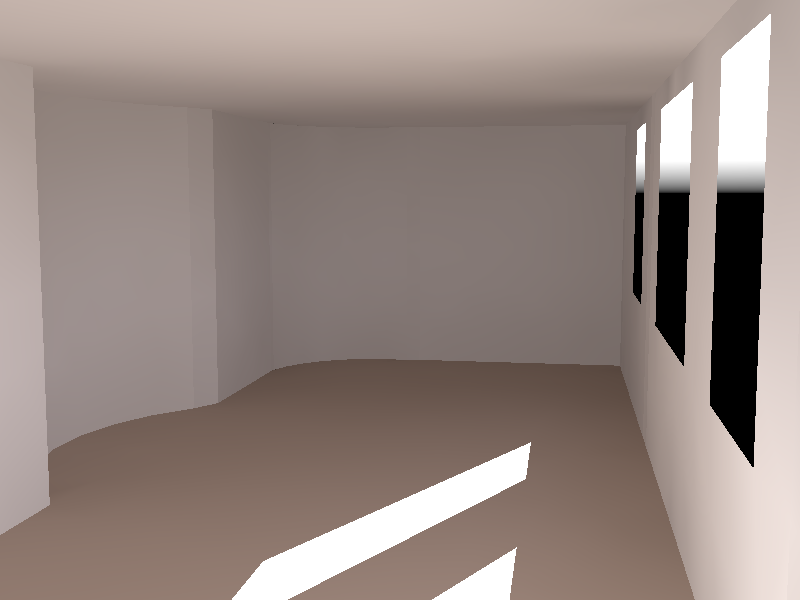
\includegraphics[width=1.62in]{../uist2012/images/creativity/C_A6_2026obj_march_CROPPED.png}
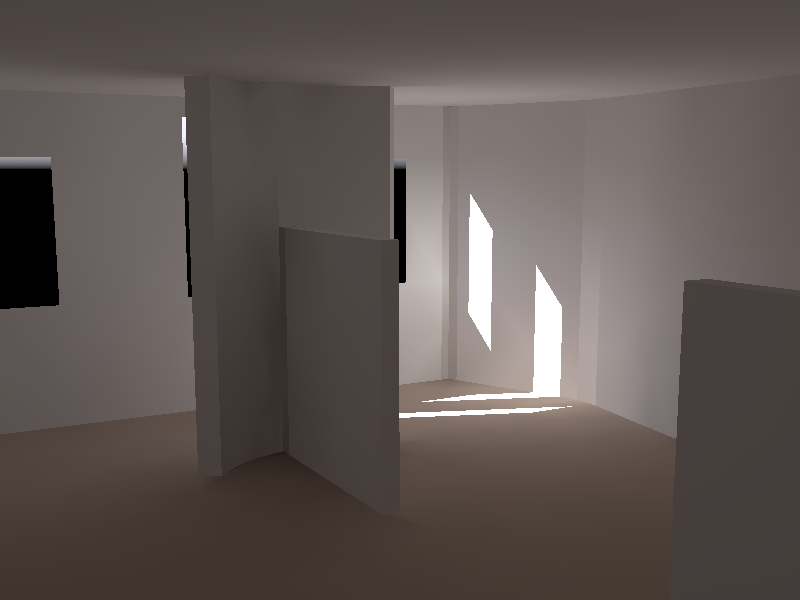
\includegraphics[width=1.62in]{../uist2012/images/creativity/C_A2_FIXED_2020obj_march_CROPPED.png}\vspace{-0.2in}\\
\begin{minipage}{1.62in}~{\color{white}{\bf A6}}\end{minipage} 
\begin{minipage}{1.62in}~{\color{white}{\bf A2}}\end{minipage}\vspace{0.05in}\\
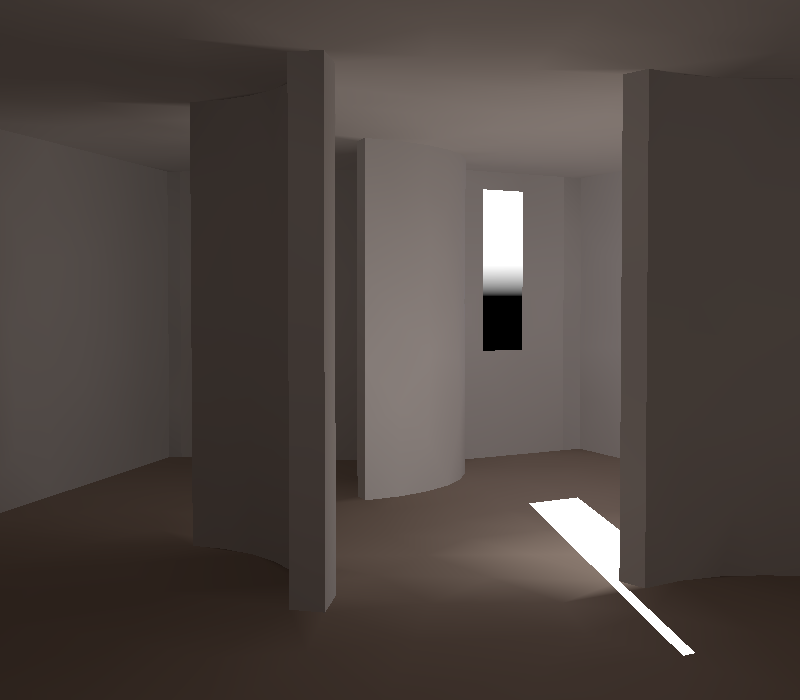
\includegraphics[width=1.62in]{../uist2012/images/creativity/C_N2_1994obj_march_CROPPED.png}
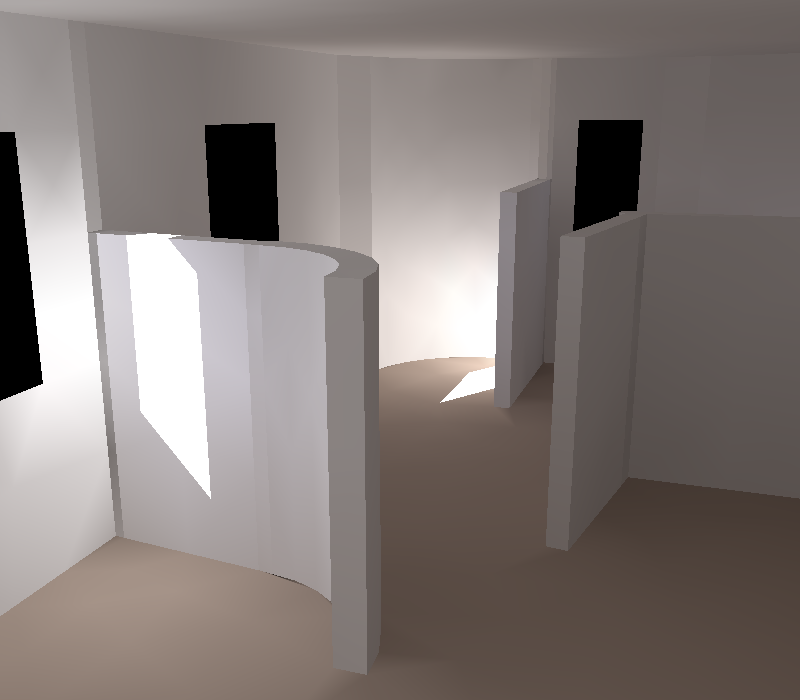
\includegraphics[width=1.62in]{../uist2012/images/creativity/C_N4_FIXED_2090obj_march_CROPPED.png}\vspace{-0.2in}\\
\begin{minipage}{1.62in}~{\color{white}{\bf N2}}\end{minipage} 
\begin{minipage}{1.62in}~{\color{white}{\bf N4}}\end{minipage}\vspace{-0.15in}\\
\caption{A sampling of the designs created by participants using a
  tangible interface.  Each model is shown lit by the sun and skylight on
  March 21st at 8:30am.
%
}
\label{figure:creativity_rendering}
\vspace{-0.1in}
\end{figure}

%\begin{figure}[t]
%  \centering
%  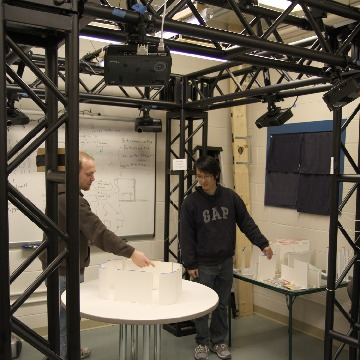
\includegraphics[width=1.65in]{../dynamic_projection/publications/gi2012_userstudy/../uist2012/images/photos/josh_jonathan_new_contraption}
%  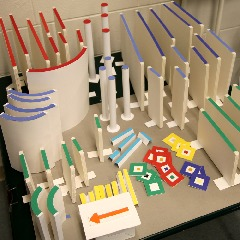
\includegraphics[width=1.65in]{../dynamic_projection/publications/gi2012_userstudy/../uist2012/images/photos/available_wall_pieces}\vspace{-0.19in}\\
%\begin{minipage}{1.65in}~{\color{white}{\bf a)}}\end{minipage}
%\begin{minipage}{1.65in}~{\color{white}{\bf b)}}\end{minipage}\vspace{0.05in}\\
%  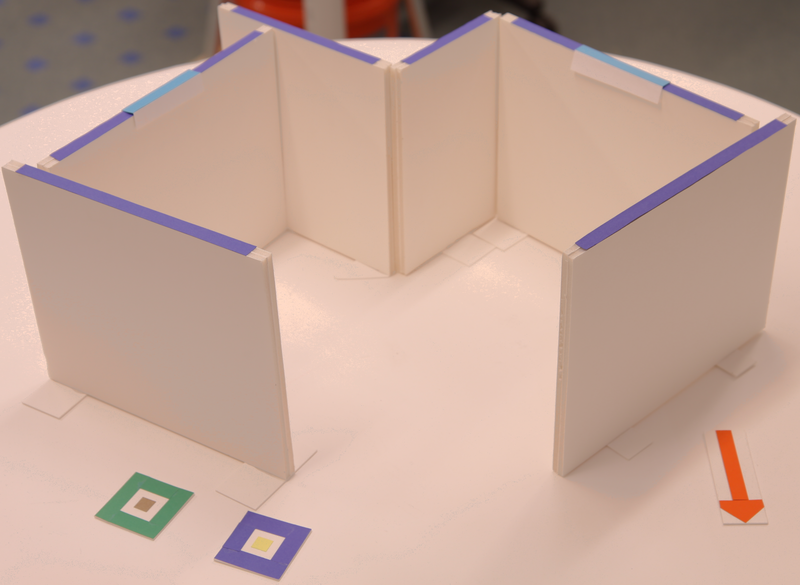
\includegraphics[width=1.65in]{../dynamic_projection/publications/gi2012_userstudy/../uist2012/images/photos/sample_model}
%  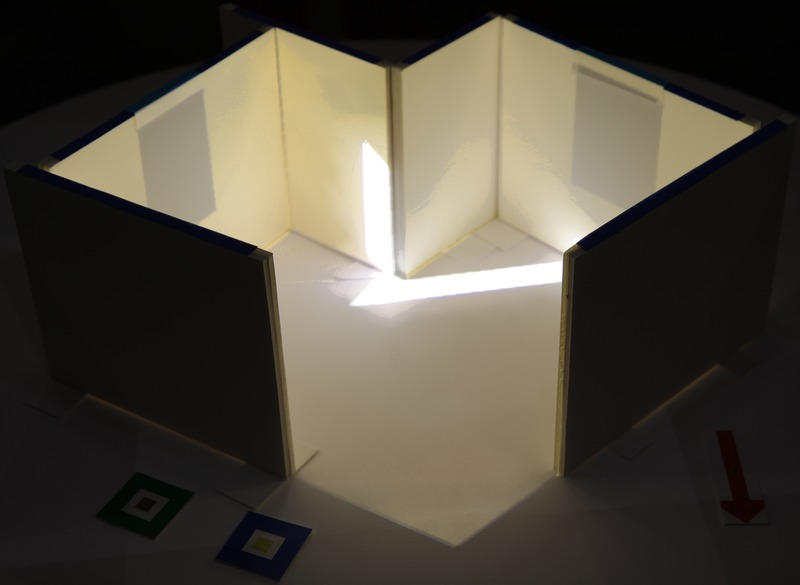
\includegraphics[width=1.65in]{../dynamic_projection/publications/gi2012_userstudy/../uist2012/images/photos/sample_rendering}\vspace{-0.19in}\\
%\begin{minipage}{1.65in}~{\color{black}{\bf c)}}\end{minipage}
%\begin{minipage}{1.65in}~{\color{white}{\bf d)}}\end{minipage}\vspace{-0.00in}\\
%  \caption{Our new TUI for architectural daylighting design allows
%    multiple users to a) gather around a physical sketching
%    environment and select from b) a set of wall primitives and window
%    and material markers to c) build a rough sketch of an
%    architectural design.  A d) visualization of a daylighting
%    simulation is projected onto these surfaces. }
%\vspace{-0.1in}
%  \label{figure:tabletop}
%\end{figure}


%In this paper we evaluate the accuracy and creativity of tangible
%interfaces in design and simulation with application to architectural
%design and daylighting simulation.  We leverage a Spatially Augmented
%Reality (SAR) user interface first introduced by \emph{Shader Lamps}
%as a way to project information onto existing surfaces in the real
%world~\cite{Raskar:2001:SLA}.  The daylighting analysis system
%simulates complex inter-reflection of natural light within a scene and
%uses a series of projectors surrounding the table to ``paint'' the
%physical primitives with the simulation results.  Designing in the
%tangible SAR system is done by sketching with physical \emph{wall
%  primitives} that are detected and interpreted to create a closed
%space.  Examples are shown in
%Figures~\ref{figure:original_designs},~\ref{figure:improved_designs},
%and~\ref{figure:new_designs} and the supplementary video.  The overall
%orientation of the sketch is specified with a \emph{north arrow
%  primitive}, windows in the model are positioned by slipping
%\emph{window primitives} over the top edge of the walls.
%
A calibrated overhead camera captures the arrangement of these
elements and the geometry is converted into a closed triangle mesh.
Radiosity, a patch-based lighting method, is used to simulate light
propagation within the space and the rendering system displays the
simulated natural lighting on the physical model using multiple
projectors positioned in a circle above the table.  The system
provides two different daylighting visualization modes: a static time
and a dynamic time-lapse animation for a whole day.  The lighting
simulation can be done for any day of the year.

The tangible daylighting interface is intended for use in the earliest
stages of architectural design, when the orientation of the building
on the site, the relative positions of rooms within the building, the
proportions of the rooms, and the placement and shape of windows is
not yet determined.  Existing commercial software for daylighting
simulation focuses on more polished and complete designs.  It can take
significant time (from minutes to hours) for the designer to construct
a digital model that both captures the current design and is suitable
for accurate and efficient simulation.  The tangible interface takes
just seconds to build or edit a model and thus is appropriate for
rough sketching and brainstorming with quick, online evaluation of
building performance.  We envision our tool being useful for a wide
audience.  Not only will it be useful for architecture students and
professional architects, but also for interior designers and future
occupants working on tasks such as furniture placement.

\noindent
The contributions of our paper: \vspace{-0.05in}

\begin{itemize}

\item Exploration of participants' fundamental understanding of
  daylighting design, overlighting, underlighting and glare.

\item Quantitative analysis of the users' accuracy in using our
  physical sketching system to model a room they had just visited.

\item Evaluation of the participants' use of our tool and their
  perception of quantitative and qualitative daylighting from the 
  displayed simulations.

\item Demonstration of our tangible interface as a
  creativity-enhancing tool for architectural daylighting design.

\end{itemize}

\subsection{Research Questions}

The common themes of education, accuracy, design, and creativity
motivated our study of the architectural daylighting system.  Our goal
was to explore the effectiveness of the tool to model specific spaces
and quantitatively users ability to evaluate the dynamic variations in
illumination.  

%
%ADDING: no traditional screen, and to explain that we a goal was to
%verify that users could interact solely with the table and still
%receive valuable feedback

\paragraph{Daylighting Intuition and Education}

An initial question we addressed was: ``How much intuition about
daylighting do people have?''  We believe that simulation TUIs are
useful both for novices who have only casual appreciation of the
dynamic qualities of light and would like to gain more general
knowledge, as well as experienced designers who want to fine tune
their understanding of the relationship between geometry and shadow.
%those who need to expand their daylighting
%knowledge as well as those with limited knowledge.  \fbox{What's the
%  difference between those groups of people?}  
We hypothesize that many users' pre-existing daylighting understanding
may be limited to general knowledge such as ``more sun in the summer''
and ``the sun travels from east to west in the sky''.  A daylighting
TUI can provide the exact path of the sunspots traveling across a
specific building geometry, problematic glare locations and times, and
the relative intensities of light as it diffusely reflects between
different surfaces and materials.  Where our study reveals common
flaws in participants' pre-existing daylighting understanding, the
tool could prove beneficial for architectural education.  Another key
question is: ``To what extent can the tool correct deficiencies in the
users' daylighting intuition?''  We hypothesize that users will have a
better overall understanding of daylighting in a variety of spaces
after using the system.

%\fbox{For this subsection, and 3.2 and 3.3 - It makes more sense}

%\fbox{to me if these descriptions are coupled with the}

%\fbox{description of the user study}


\paragraph{Modeling and Simulation Accuracy}


The accuracy of a daylighting simulation is dependent upon the
precision of the model built by the users.  If the designer is sloppy
in specifying the proportions of the room or windows, the orientation
of the building, or the material properties, the resulting simulation
may over- or under-estimate the daylighting.  We ask the question:
``How accurate are users at understanding and recreating with a TUI a
space they have visited and sketched?''
%
The accuracy of a simulation is also dependent upon attention to
details that have the most significant impact on the lighting
calculations.  ``Do users identify and accurately reproduce features
of a space significant in daylighting simulation, i.e., interior
partitions, window dimensions, and ceiling height?''
%
Finally, the accuracy of our TUI is ultimately dependent upon the
display and perception of the simulation results.  ``Do the users
accurately perceive and interpret the displayed information?''  
%We
%investigate both the accuracy of proportions and attention to details
%in this study.  We also study the users' response and interpretation
%of the daylighting visualization.

\begin{figure}[t]
\centering
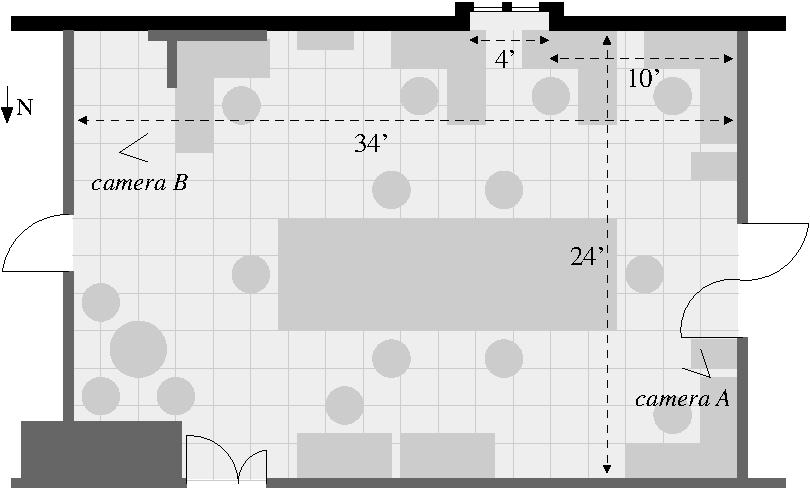
\includegraphics[width=2.5in]{../gi2012_userstudy/images/lab.pdf} \vspace{0.1in}
\\
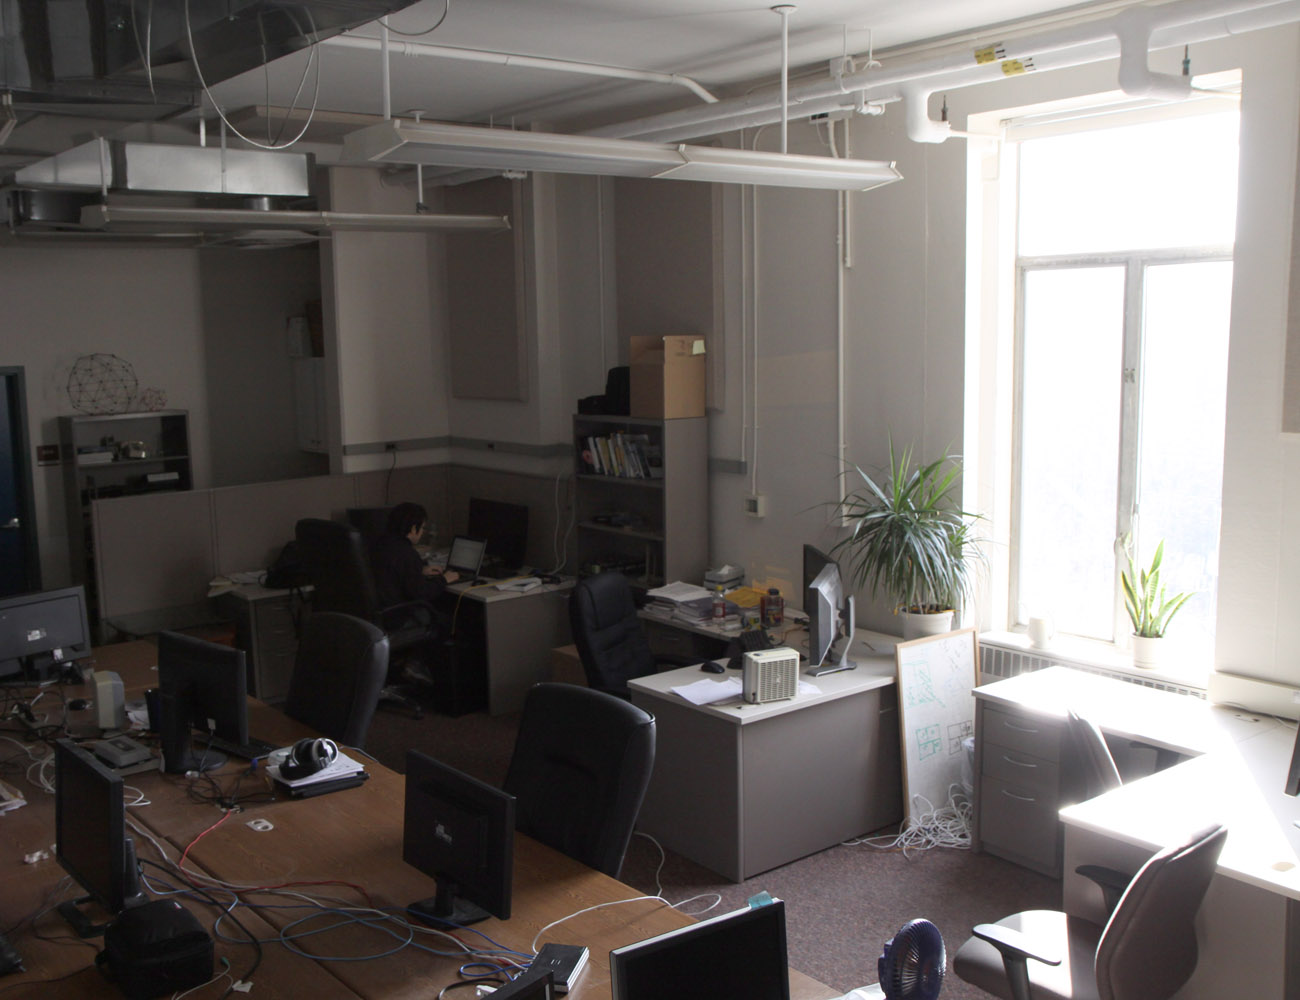
\includegraphics[width=1.65in]{../gi2012_userstudy/images/photos/camera_angle_2_lights_off.jpg}
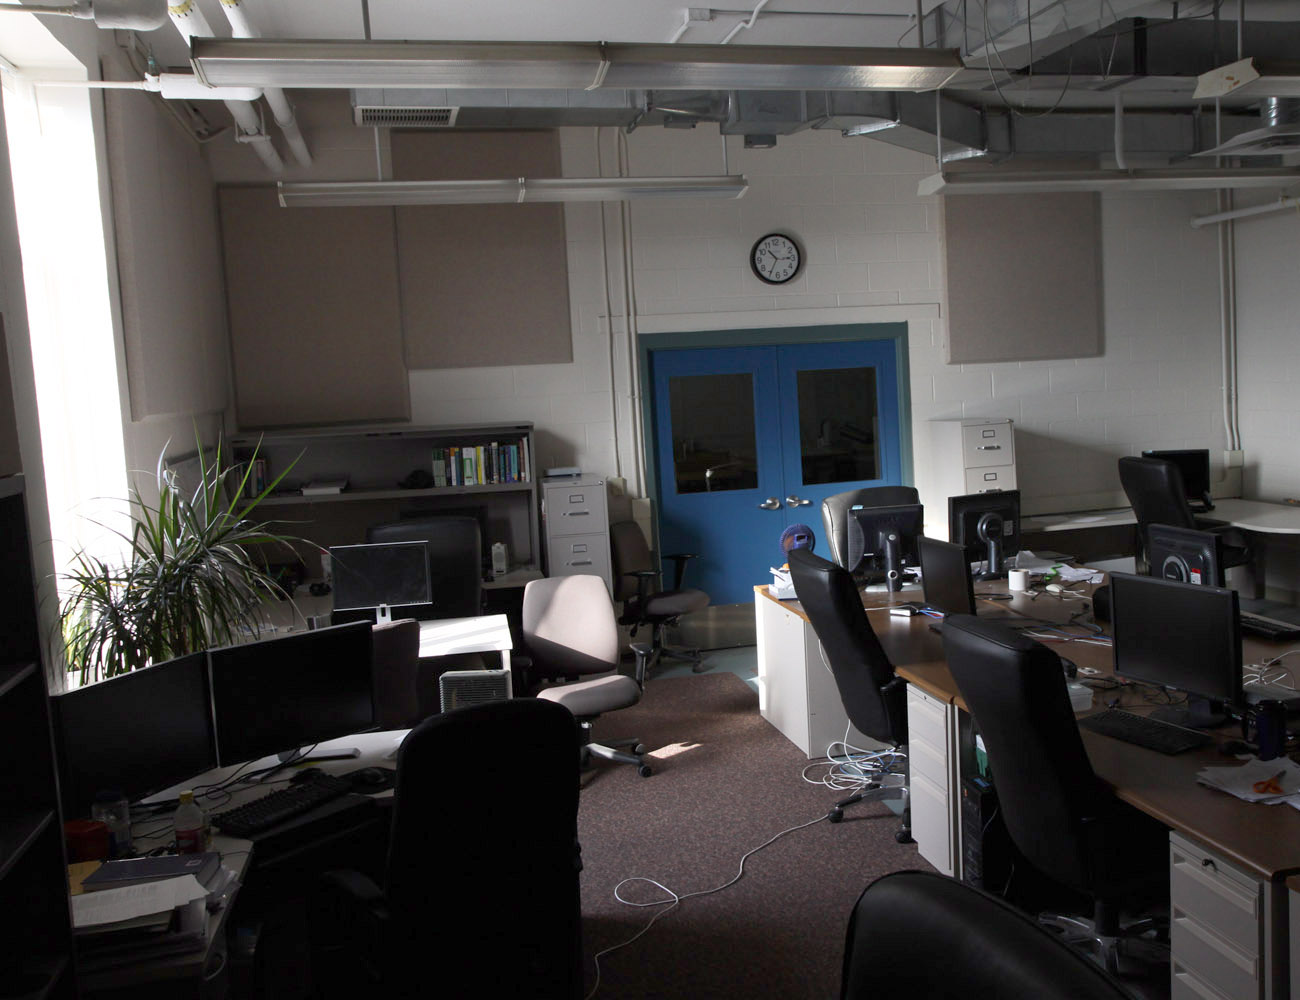
\includegraphics[width=1.65in]{../gi2012_userstudy/images/photos/camera_angle_3_lights_off.jpg}\vspace{-0.19in}\\
%\begin{minipage}{1.65in}~{\color{white}{\em camera A, lights off}}\end{minipage}
%\begin{minipage}{1.65in}~{\color{white}{\em camera B, lights off}}\end{minipage}\vspace{0.05in}\\
\begin{minipage}{1.65in}~{\color{white}{\em camera A}}\end{minipage}
\begin{minipage}{1.65in}~{\color{white}{\em camera B}}\end{minipage}\vspace{0.0in}\\
%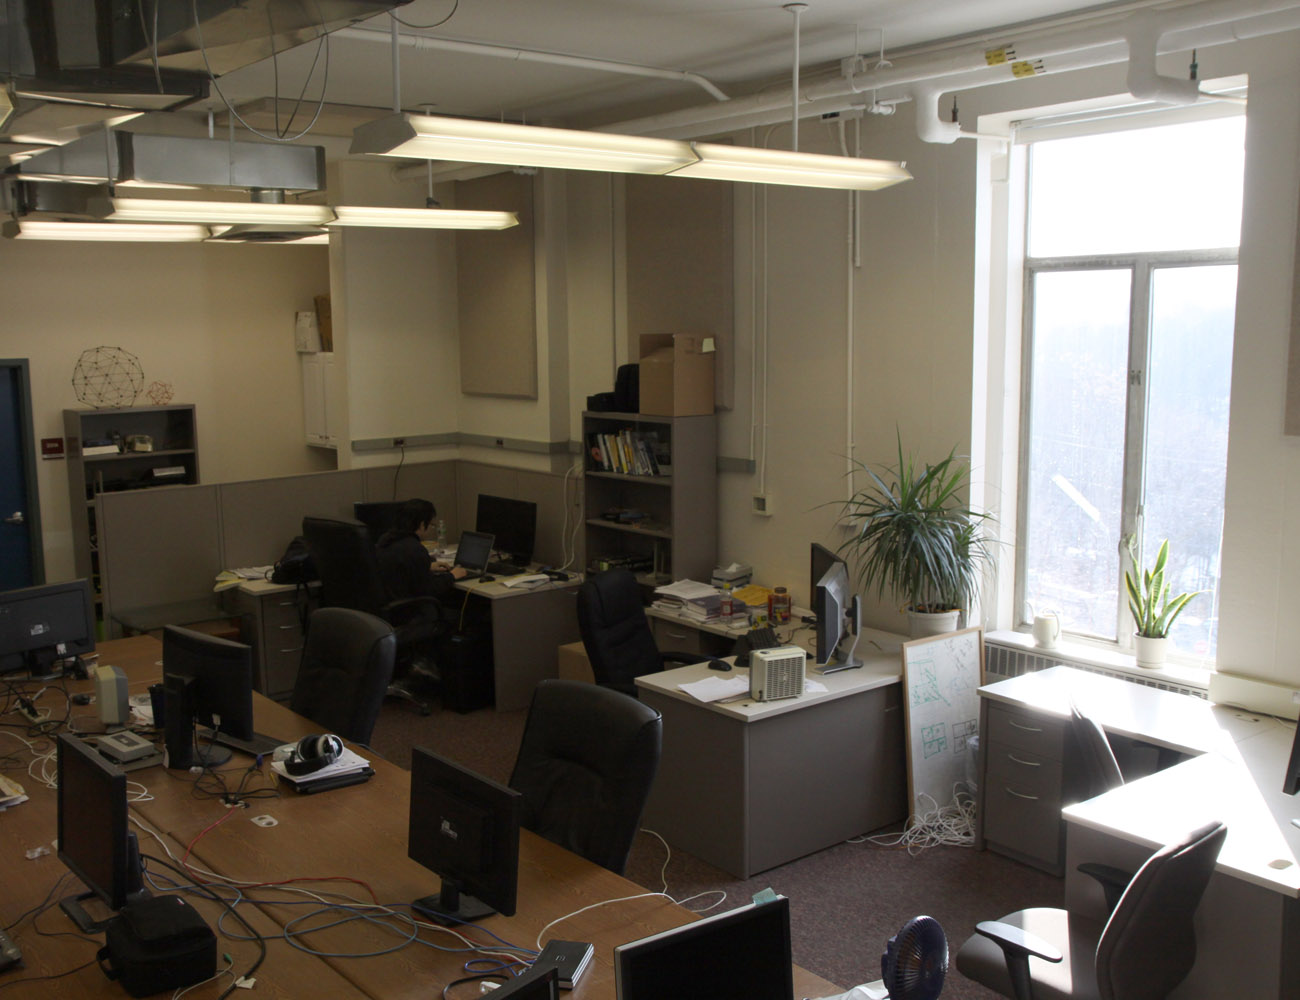
\includegraphics[width=1.65in]{../dynamic_projection/publications/dynamic_projection/publications/gi2012_userstudy/images/photos/camera_angle_2_lights_on.jpg}
%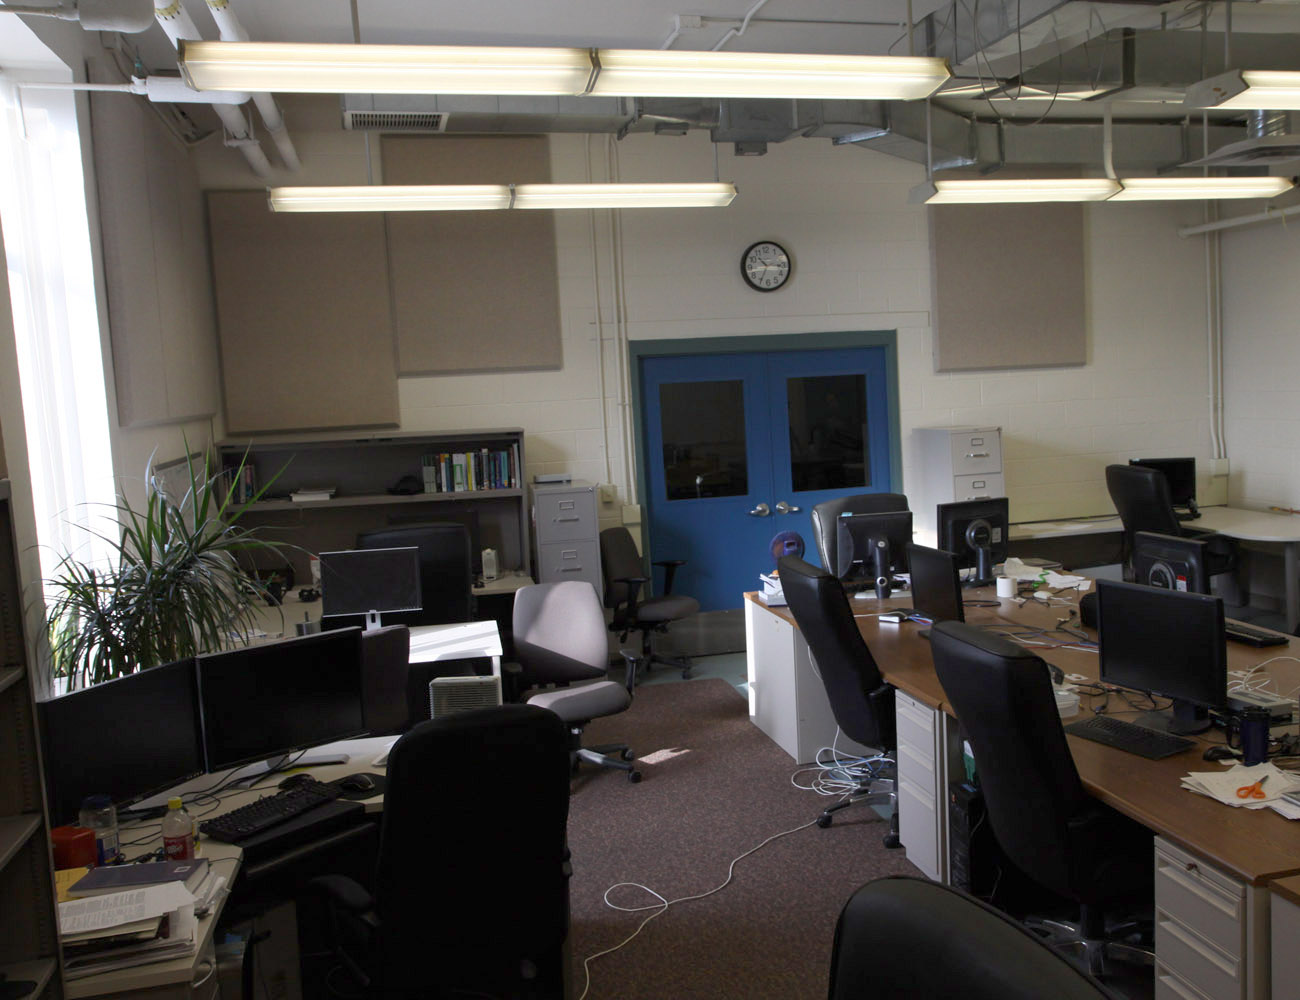
\includegraphics[width=1.65in]{../dynamic_projection/publications/dynamic_projection/publications/gi2012_userstudy/images/photos/camera_angle_3_lights_on.jpg}\vspace{-0.19in}\\
%\begin{minipage}{1.65in}~{\color{white}{\em camera A, lights on}}\end{minipage}
%\begin{minipage}{1.65in}~{\color{white}{\em camera B, lights on}}\end{minipage}\vspace{0.00in}\\
\caption{User study participants visited this simple open office
  environment as a case study for daylighting analysis.  The room
  contains a single, tall and narrow, south-facing window that
  provides direct overly-intense illumination to portions of the room
  while leaving other areas relatively dark.  Thus, occupants of the
  space typically turn on the overhead lights, and on sunny afternoons
  a diffusing shade is needed to prevent glare.
% even on sunny
%  afternoons.
}
\label{figure:example_room}
\end{figure}




\begin{figure*}[t]
%
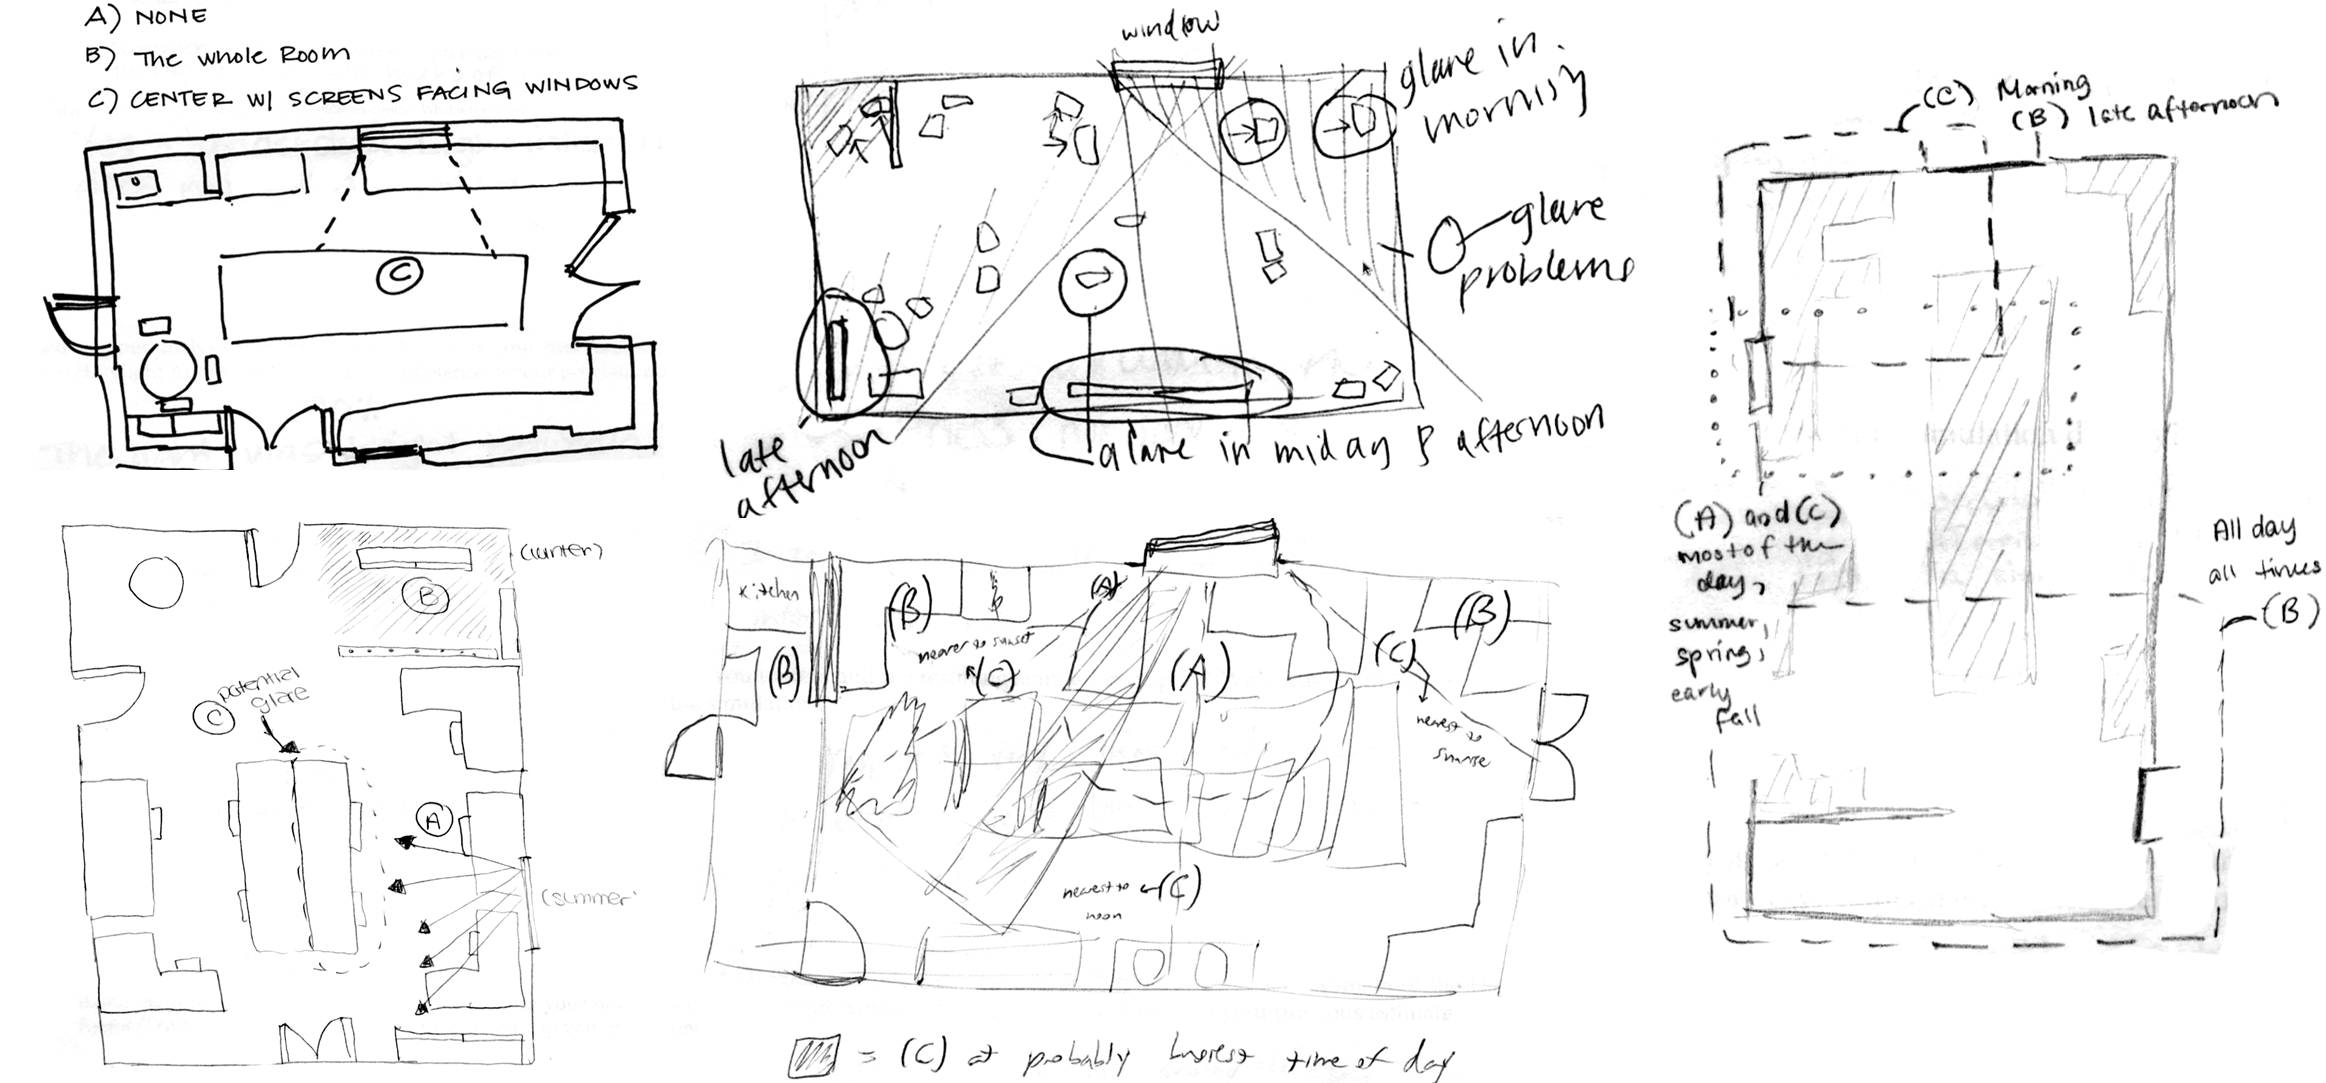
\includegraphics[width=7.0in]{../gi2012_userstudy/images/sketches/all_together}%
%
\vspace{-2.7in}
{\bf A4} \hspace{1.9in}
{\bf A3}
\vspace{2.3in}
\\
{\bf A5} \hspace{1.8in}
{\bf N2} \hspace{3in}
{\bf N4}
\vspace{-0.1in}\\
%
\caption{In Part 1 of the study, participants were asked to sketch the
  lab room and annotate this sketch with their intuition about areas
  with A) too much daylighting, B) too little daylighting, and C)
  potential for glare.  The sketches demonstrate a variety of detail
  and accuracy in the analysis of the dynamic lighting conditions. }
\label{figure:sketches}
\end{figure*}







\paragraph{Creativity and Architectural Design }

Informal presentation of a daylighting TUI to architects and
non-architects, support the hypothesis that users can effectively and
creatively design using this tool.  A fundamental question of our
evaluation: ``How is this tangible tool useful in the architectural
design process?''  We predict that users will appreciate the
simplicity of the model construction and speedy production and display
of simulation results.  Furthermore, we predict that when users are
presented with this more complete and detailed representation of
daylighting, they will embrace the benefits of using such a tool
regularly, and use insights gained through tool use to modify their
designs.  %We also wish to investigate if users feel creative freedom
%within the tool.  
Additionally, we wish to investigate: ``Is users' creativity catalyzed
by using the tool?'' and ``Do users feel particular constraints in design
because of the tool?''  


\subsection{User Study Design and Protocol}


The TUI for daylighting analysis and design is targeted to
professional architects, architecture students, and may be beneficial
for clients and other design fields as well.  Because our tool does
not require much training to use, we claim it is a valuable general
educational tool for daylighting.  To answer the questions outlined in
the previous sections, we recruited a pool of thirteen university
students.  Six of the users were architecture students (labeled
A1-A6), all with at least two years of formal architecture education
and seven students from other departments (labeled N1-N7), but many
with a background in electronic media, arts, and communication (5
students) or games studies (1 student).

Our study was divided into four consecutive tasks.  The first task was
designed to prime the user for thinking about daylighting and gauge
the user's pre-existing intuitions.  The other three tasks had the
participant work with the TUI daylighting simulation system.  Thus,
prior to the second task, a brief, 5-minute introduction to the system
was provided.  The second, third, and fourth tasks of the study were
designed in the spirit of a \emph{cognitive walkthrough}, but with
guidance on tool use available during the study and a self-reflective
pen-and-paper questionnaire completed by the user after each task.
Users were allowed to experiment with the system as they saw fit in
completing each task.
%
Each section began with brief explanation (1-2 minutes), open
exploration time with the tool in which participants create 1 or more
models and view multiple daylighting simulations (5-20 minutes), and
culminated with a questionnaire (10 minutes).  Users were encouraged
to ask questions or provide feedback about the tool at any time.  The
tasks were designed such that the study took approximately 1 to 2
hours in total.  This user study was each participant's first use
of the tangible user interface for daylighting simulation.

A short handout for users, the questionnaire, and the user study
script (read aloud to each participant) is provided in a supplementary
document.


%was the participants first use of this
%daylightingpants this was
%their first use of the daylighting simulation visualization aspects of
%the tool.

%%%%%%%%%%%%%%%%%%%%%%%%
%%%%%%%%%%%%%%%%%%%%%%%%
%%%%%%%%%%PUT THIS BACK IN WHEN WE GET ACCEPTED...
%%%%%%%%%%%%%%%%%%%%%%%%
%%%%%%%%%%%%%%%%%%%%%%%%
%Some of the users had participated in an earlier study on construction
%of physical sketches and recognition and interpretation of the physical
%sketch geometry
%%~\cite{aag201015} 
%\fbox{can't ref ourselves}, but for all participants this was
%their first use of the daylighting simulation visualization aspects of
%the tool.


  %\fbox{ Can you figure out who had used the modeling portion
  %of the tool before and mark them in the proportions table?  did
  %prior users model more accurately? }
% Should fix this but low priority

% UNFORTUNATELY just reading the instructions is not the same as play
%time building shapes 
%
% In order to emulate the same amount of exposure
%for all participants, we also read the instructions on operating the
%system as in previous user studies to participants who were getting
%their first exposure to the system.






\paragraph{Part 1: Daylighting Intuition for Existing Space}

The aim of the first part of the study is to reveal the participant's
intuition about daylighting and provide the user a basis for
self-evaluation.  The study begins with a tour of an open office space
seating twelve graduate students with desktop computers and monitors
(Figure~\ref{figure:example_room}).  This room was selected for its
simple geometry yet non-uniform daylighting from a single south-facing
window.  Portions of the room are gloomily dark while other areas
receive direct illumination on the desk surfaces and computer
monitors.  Thus, this space is a good illustration of the need for
careful analysis during design to maximize use of illumination from
the sun and sky and minimize glare.  The user is provided a handout
with basic measurements of the space at the start of the tour.

The user is asked to identify areas in the room with too much or too
little daylighting as well as the locations with glare, and to also
specify daily and seasonal variations.  Once the user has explored the
room, he is asked to draw an annotated sketch of the room showing poor
or problematic natural lighting (Figure~\ref{figure:sketches}).  The
sketch allows us to understand the complexity and accuracy of their
daylighting intuitions.  Similarly, the questionnaire for Part 1
focused on the user's pre-existing understanding of daylighting.  We
asked the user to estimate the space's daylight autonomy and note the
weather conditions and use of electric lighting in the room at the
time they did the study.  This gave us an idea of their prior
knowledge as well as any bias from the specific lighting conditions
during their visit.

Each user spent 10-15 minutes in the space during this part of the
study.  They were free to walk around the space and explore different
viewpoints and then sit at a desk in the room to complete their
annotated sketch of the room and fill out the first part of the
questionnaire.


\paragraph{Part 2: Using the TUI to Analyze Existing Space}

For the second part of the study, users were introduced to the TUI
system for daylighting simulation.  The participant constructs a
physical model of the computer lab they just visited and sketched.
The user has access to the provided room measurements as well as their
sketch and notes.  Then, the participant is invited to use the TUI
simulation visualizations to evaluate the natural illumination,
requesting multiple static time or timelapse animations of particular
days of the year.  By examining their choice of times and days
selected, we can quantify the thoroughness of their exploration, and
their understanding of the summer and winter solstice and the fall and
spring equinox, and sunrise and sunset.

In addition to comparing the simulations with their earlier
predictions, the questionnaire for this section also asked them to
re-estimate the daylight autonomy of the space and discuss their
understanding and perception of the simulation display.  The first two
parts of the study provide insight into the value of our tool as an
educational interface as it evaluates users' perceptions both before
and after utilizing the tool to evaluate daylighting within a simple
geometry that they had personally visited.



\begin{figure*}[t]
\begin{center}
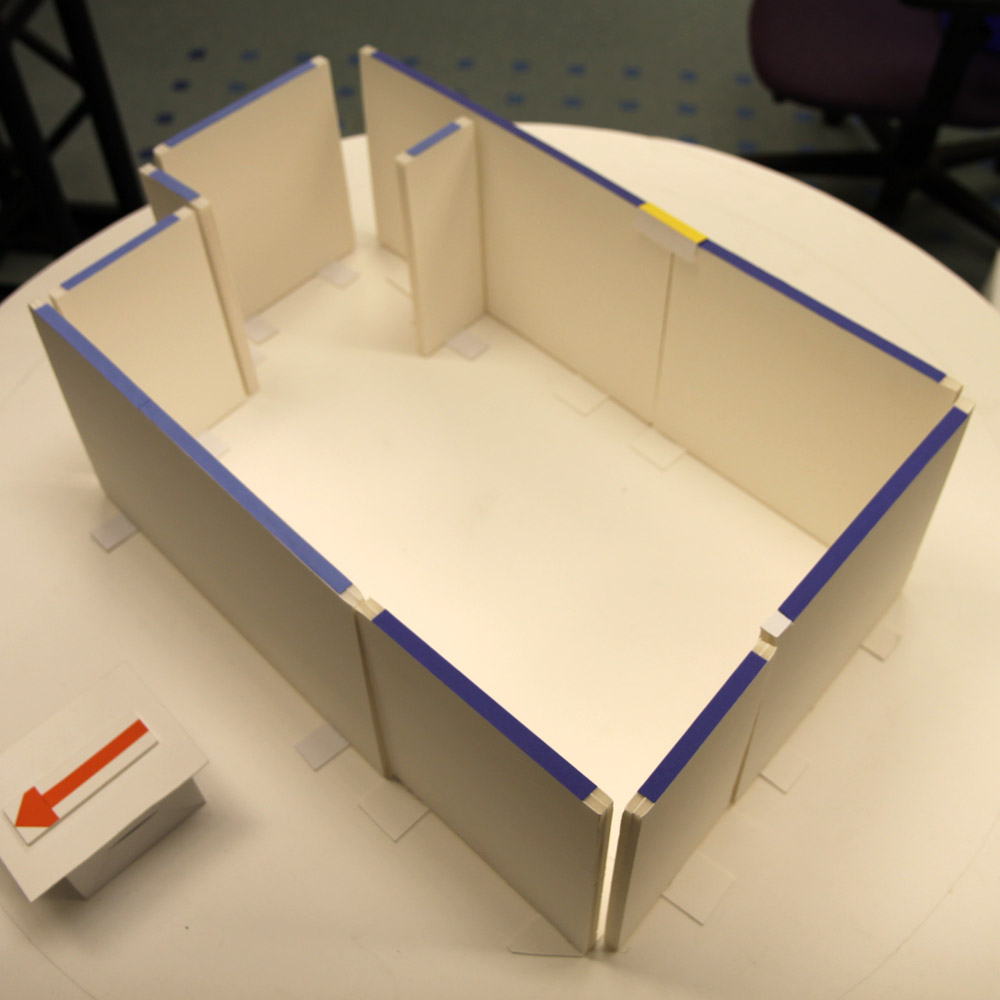
\includegraphics[width=1.4in]{../gi2012_userstudy/images/photos/63_original} %N1
\begin{minipage}[b]{3.7in}
  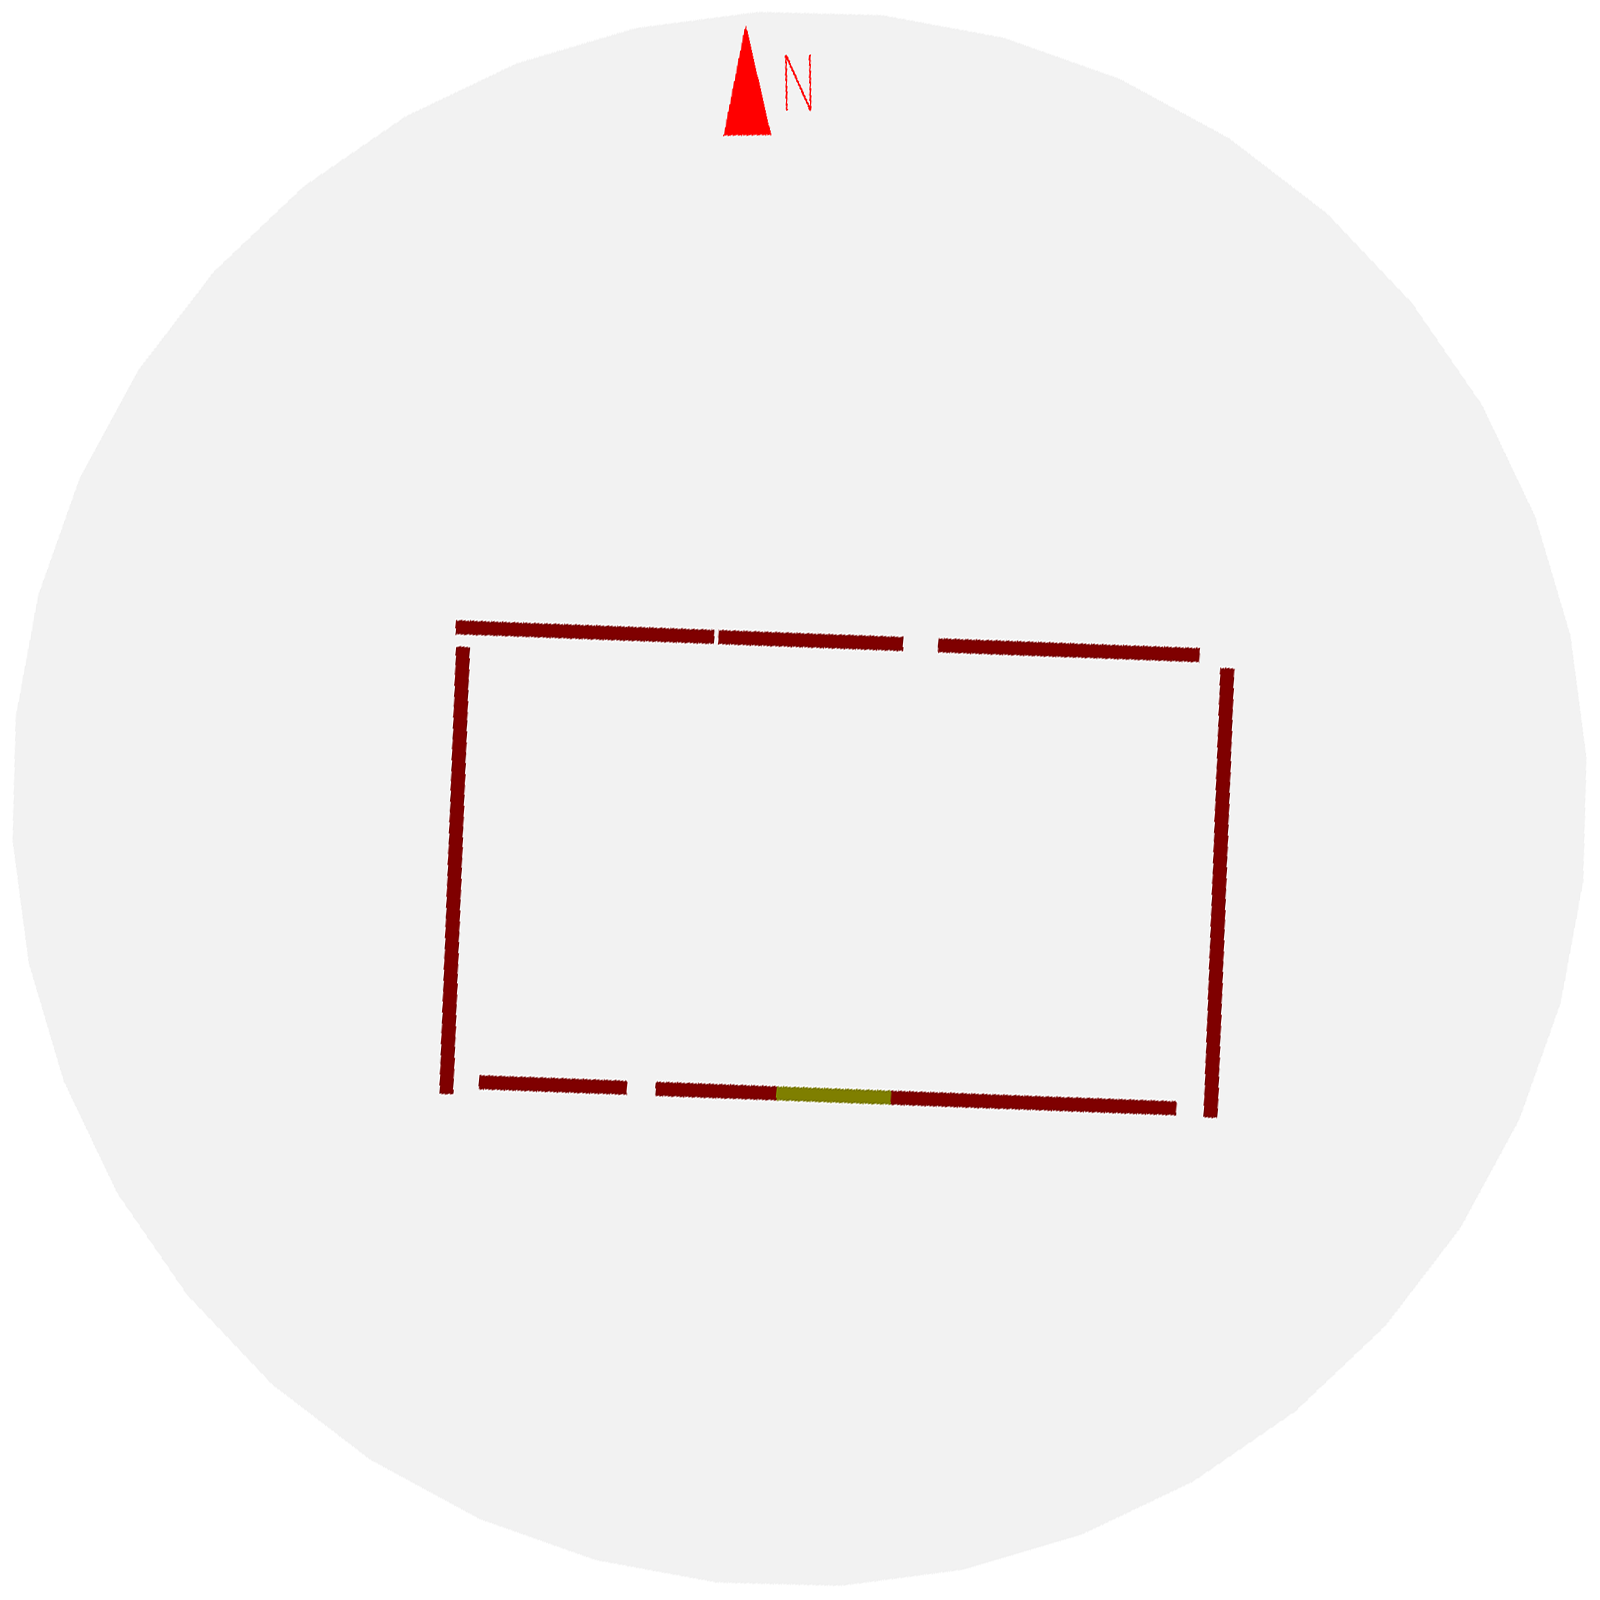
\includegraphics[width=0.7in]{../gi2012_userstudy/images/section2/0_2D_walls_rotate} %A1
  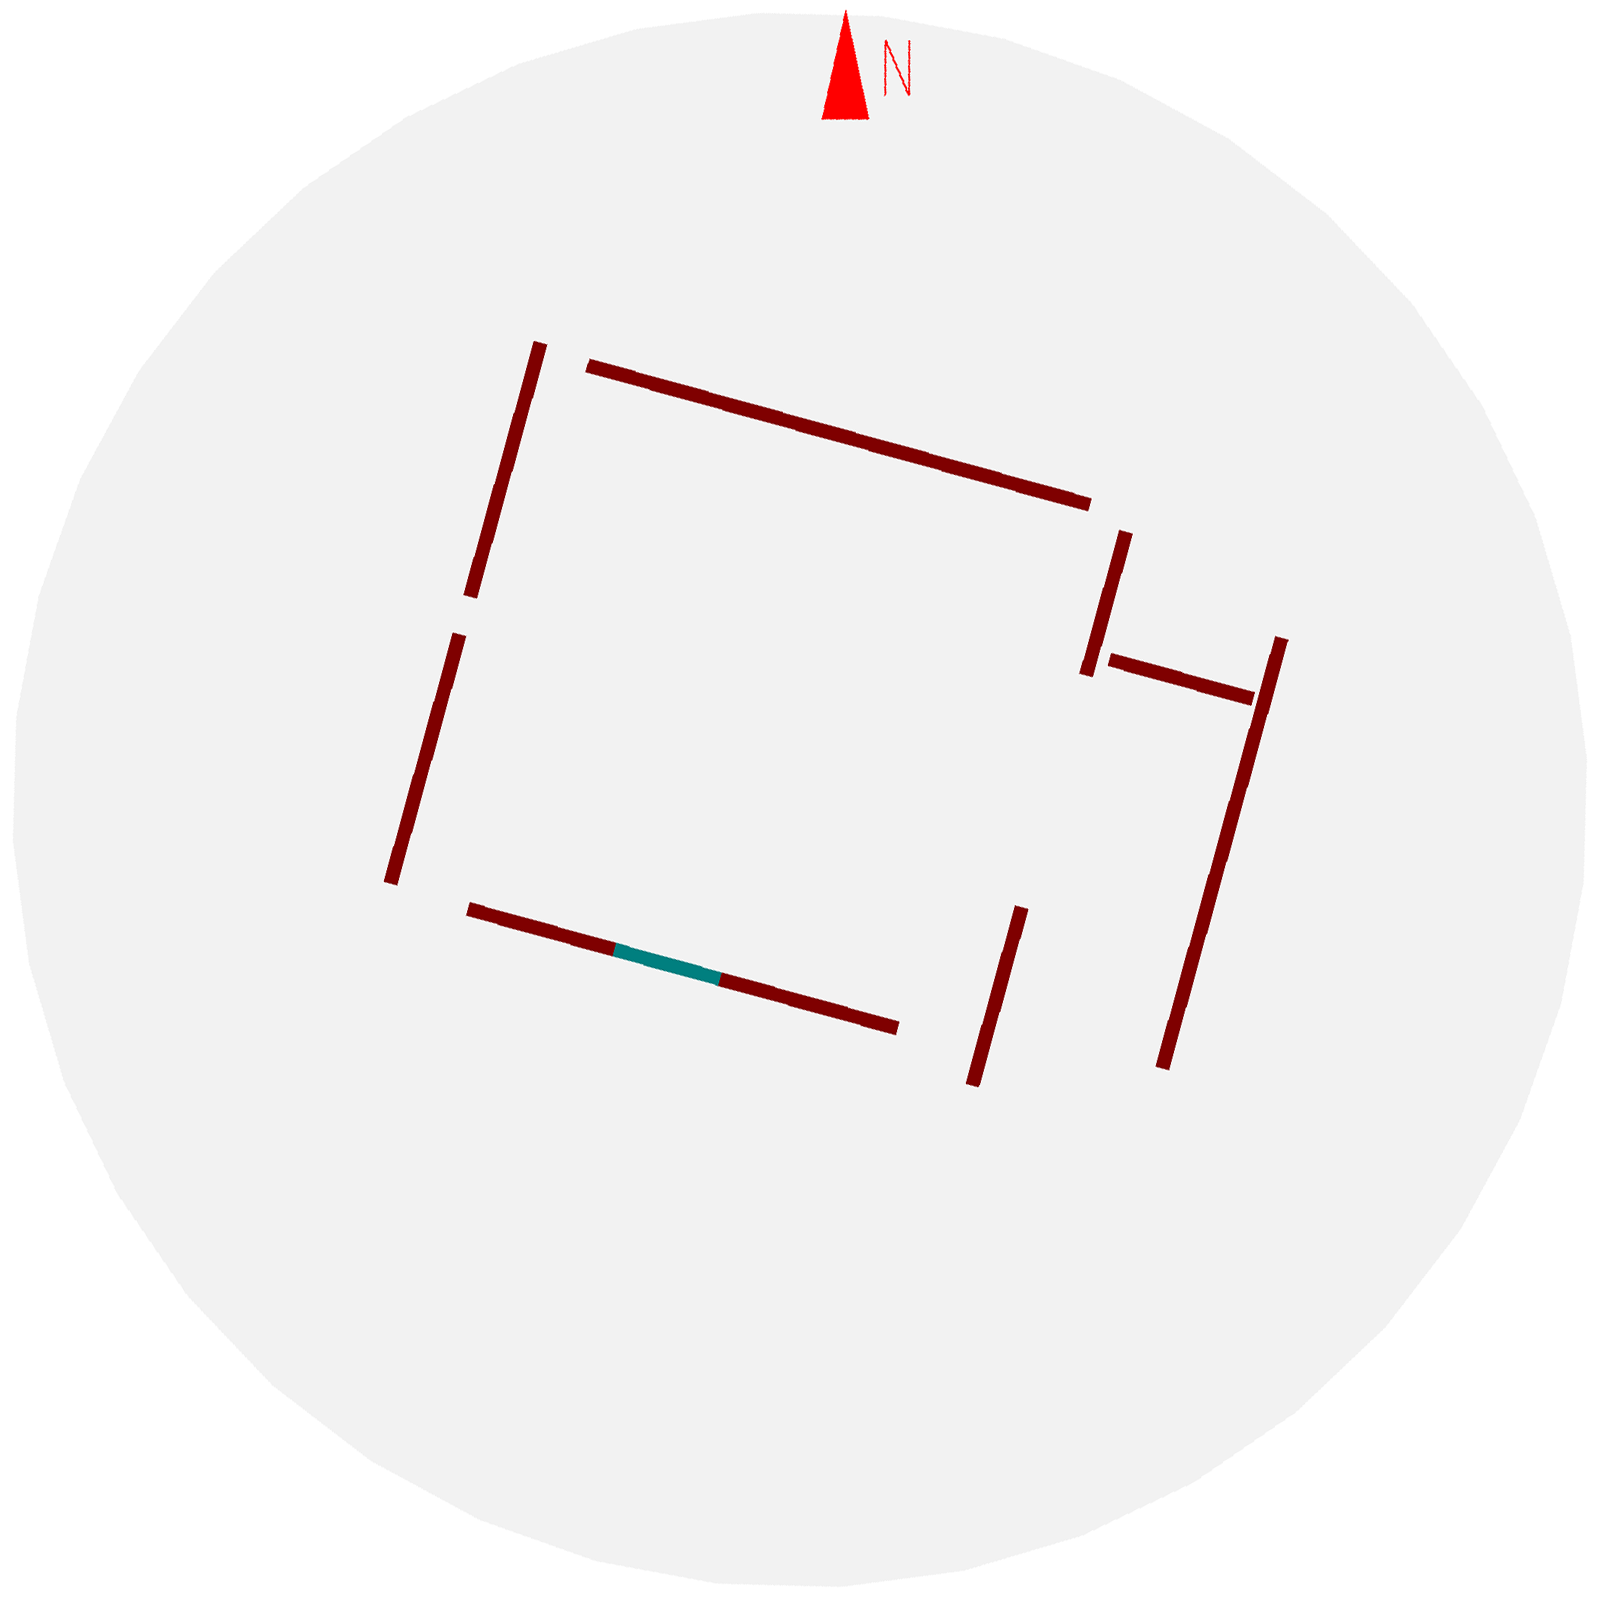
\includegraphics[width=0.7in]{../gi2012_userstudy/images/section2/2_2D_walls_rotate} %A2
  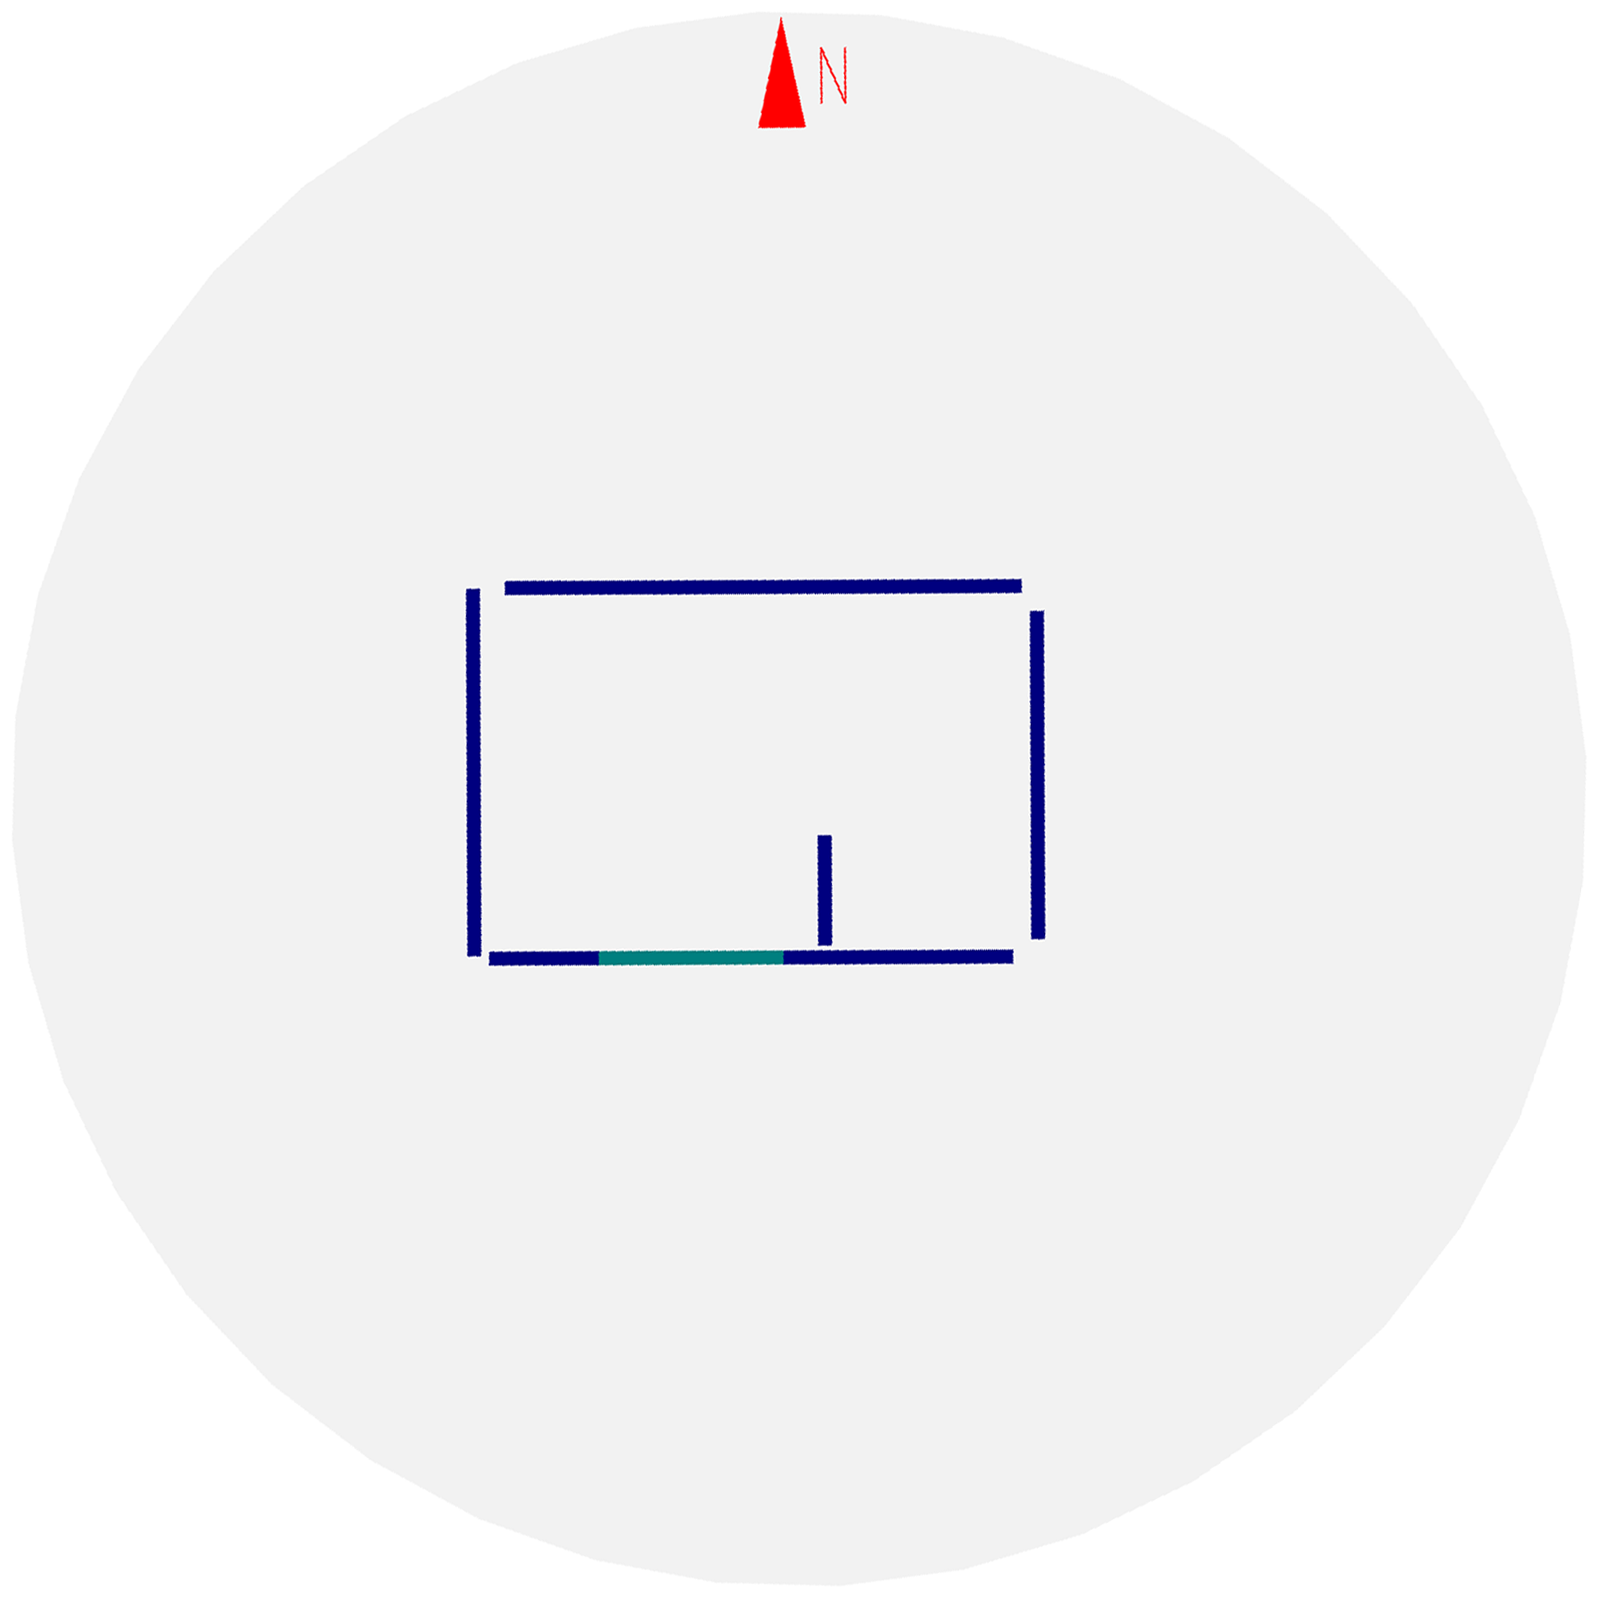
\includegraphics[width=0.7in]{../gi2012_userstudy/images/section2/6_2D_walls_rotate}  %A4
  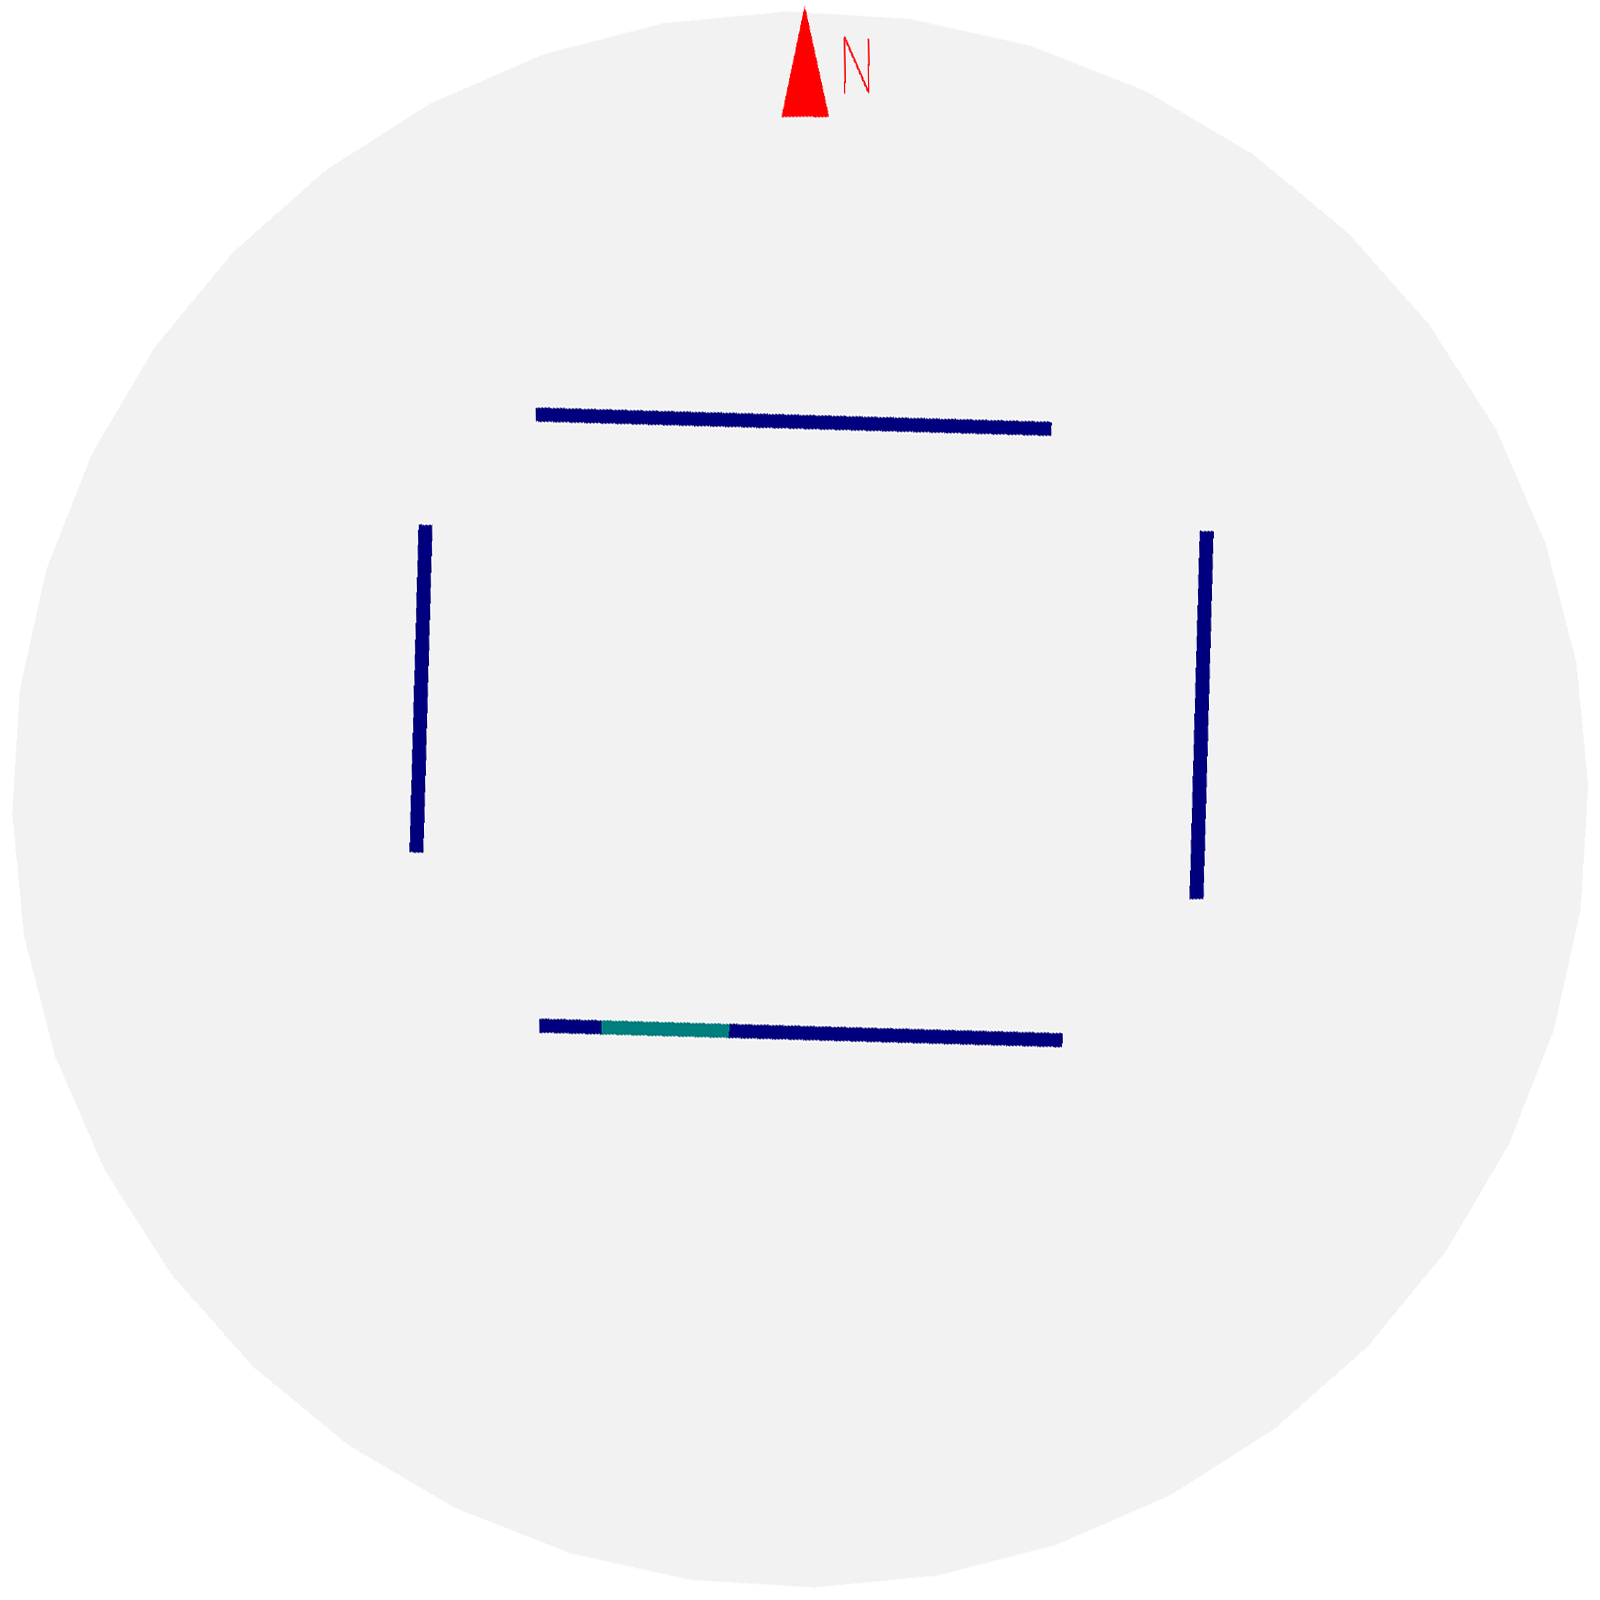
\includegraphics[width=0.7in]{../gi2012_userstudy/images/section2/7_2D_walls_rotate} %A5
  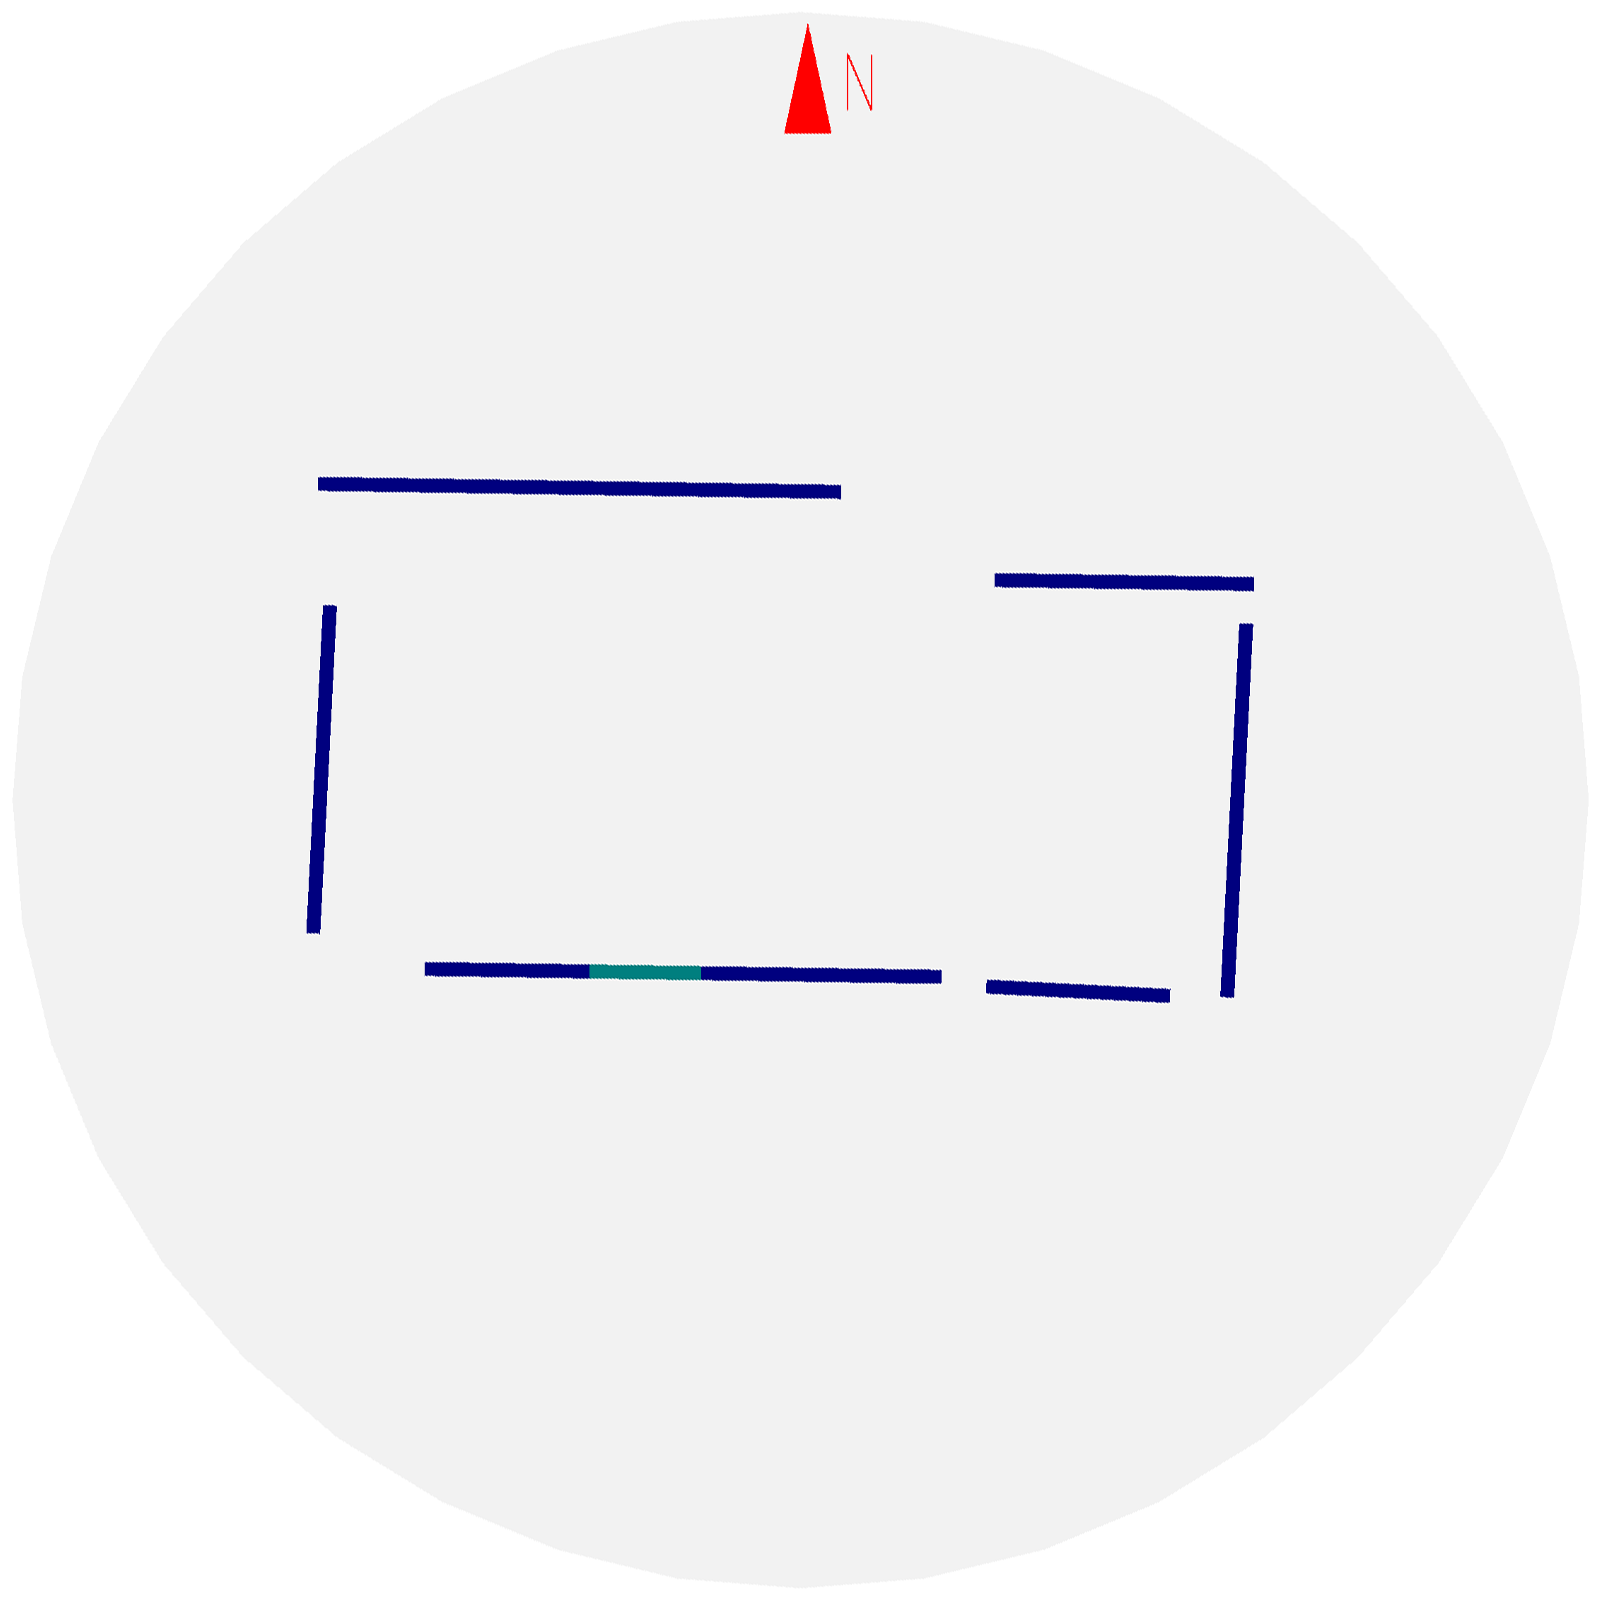
\includegraphics[width=0.7in]{../gi2012_userstudy/images/section2/8_2D_walls_rotate}\\ %A6
  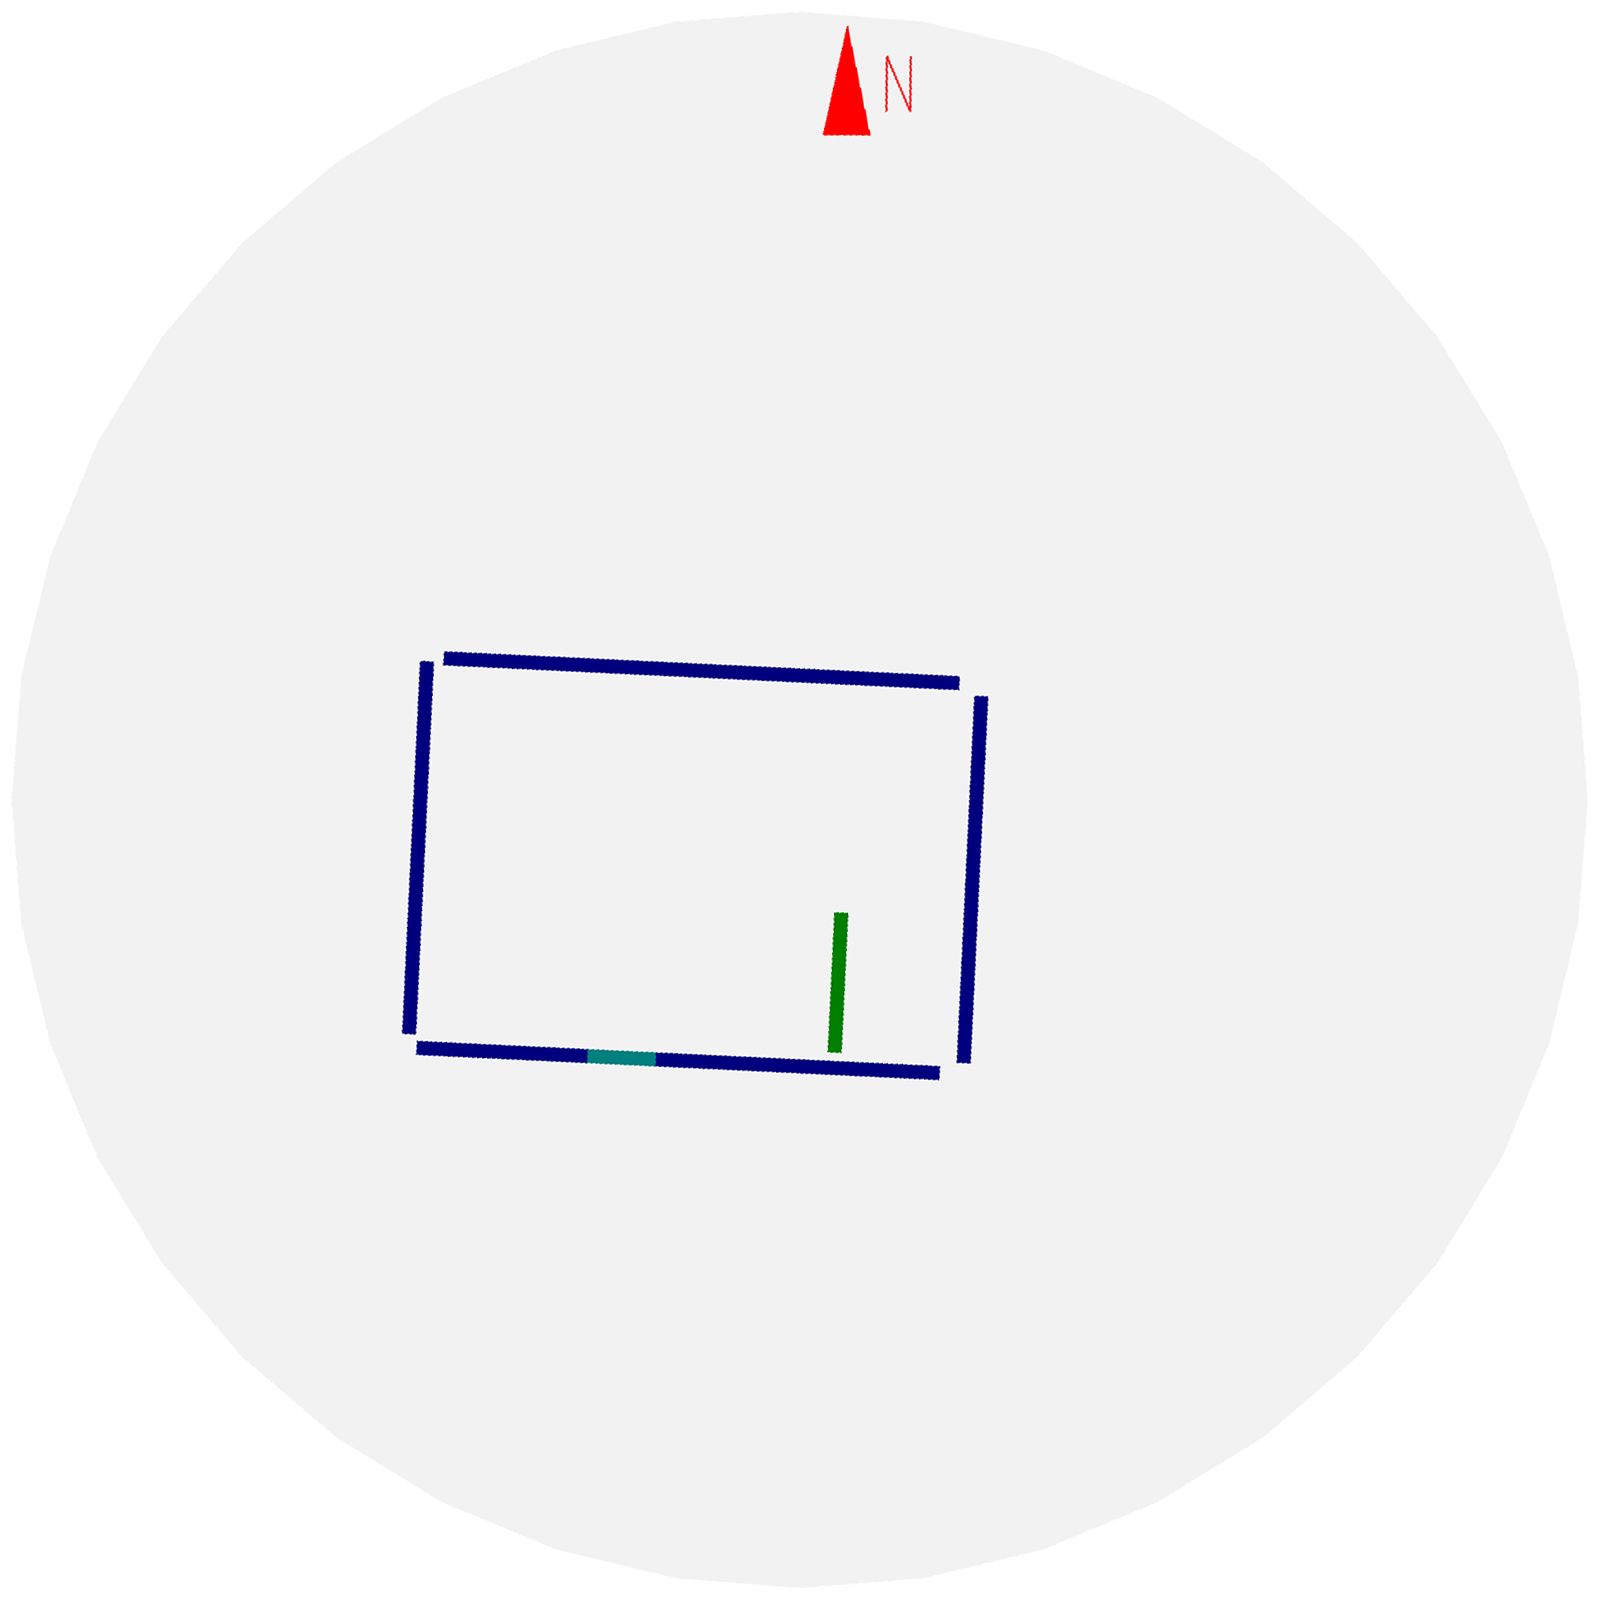
\includegraphics[width=0.7in]{../gi2012_userstudy/images/section2/3_2D_walls_rotate} %N2
  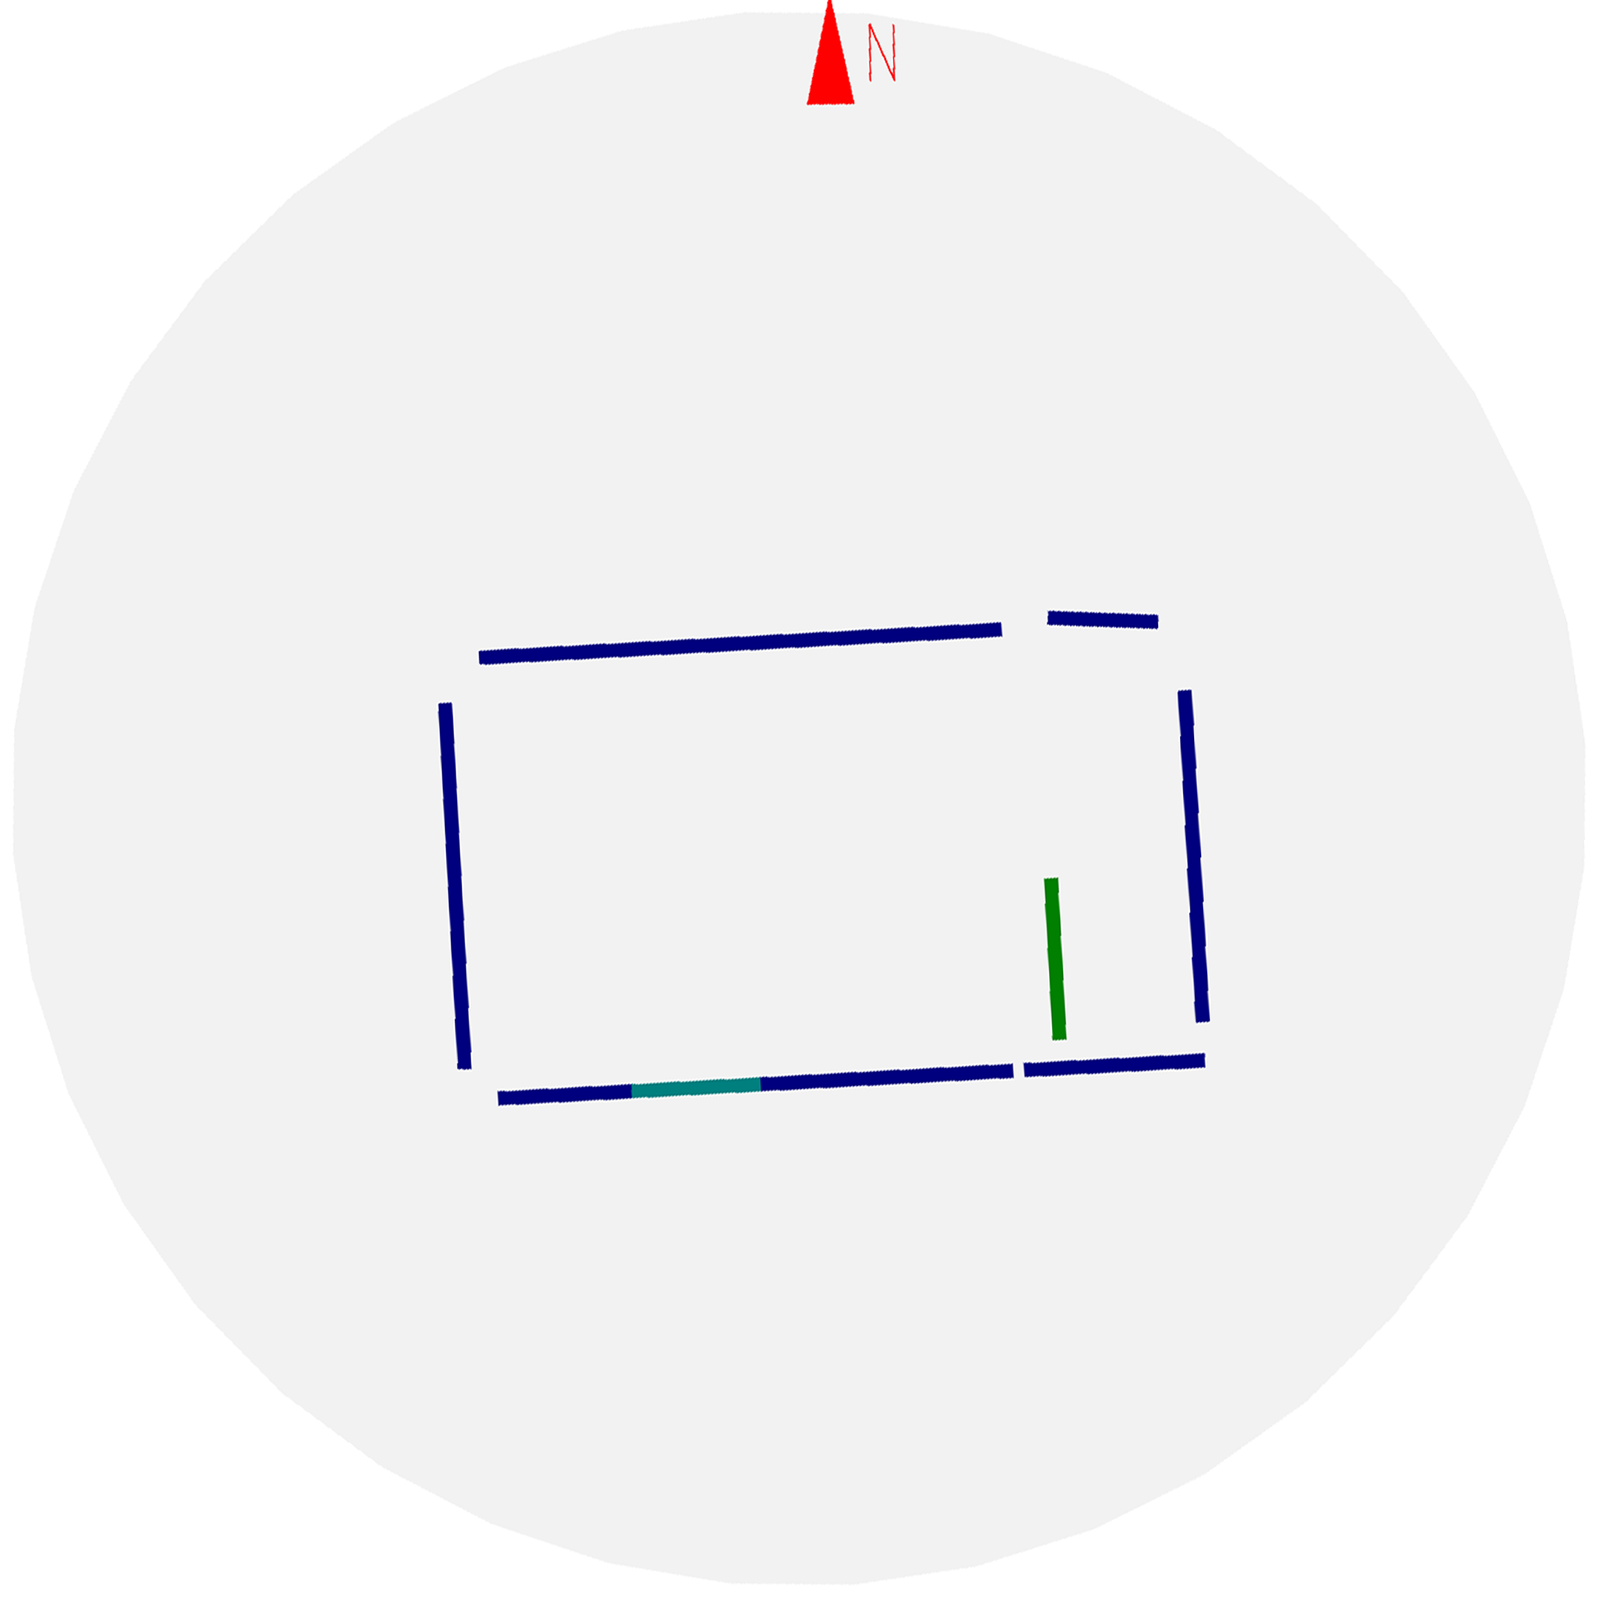
\includegraphics[width=0.7in]{../gi2012_userstudy/images/section2/5_2D_walls_rotate} %N4
  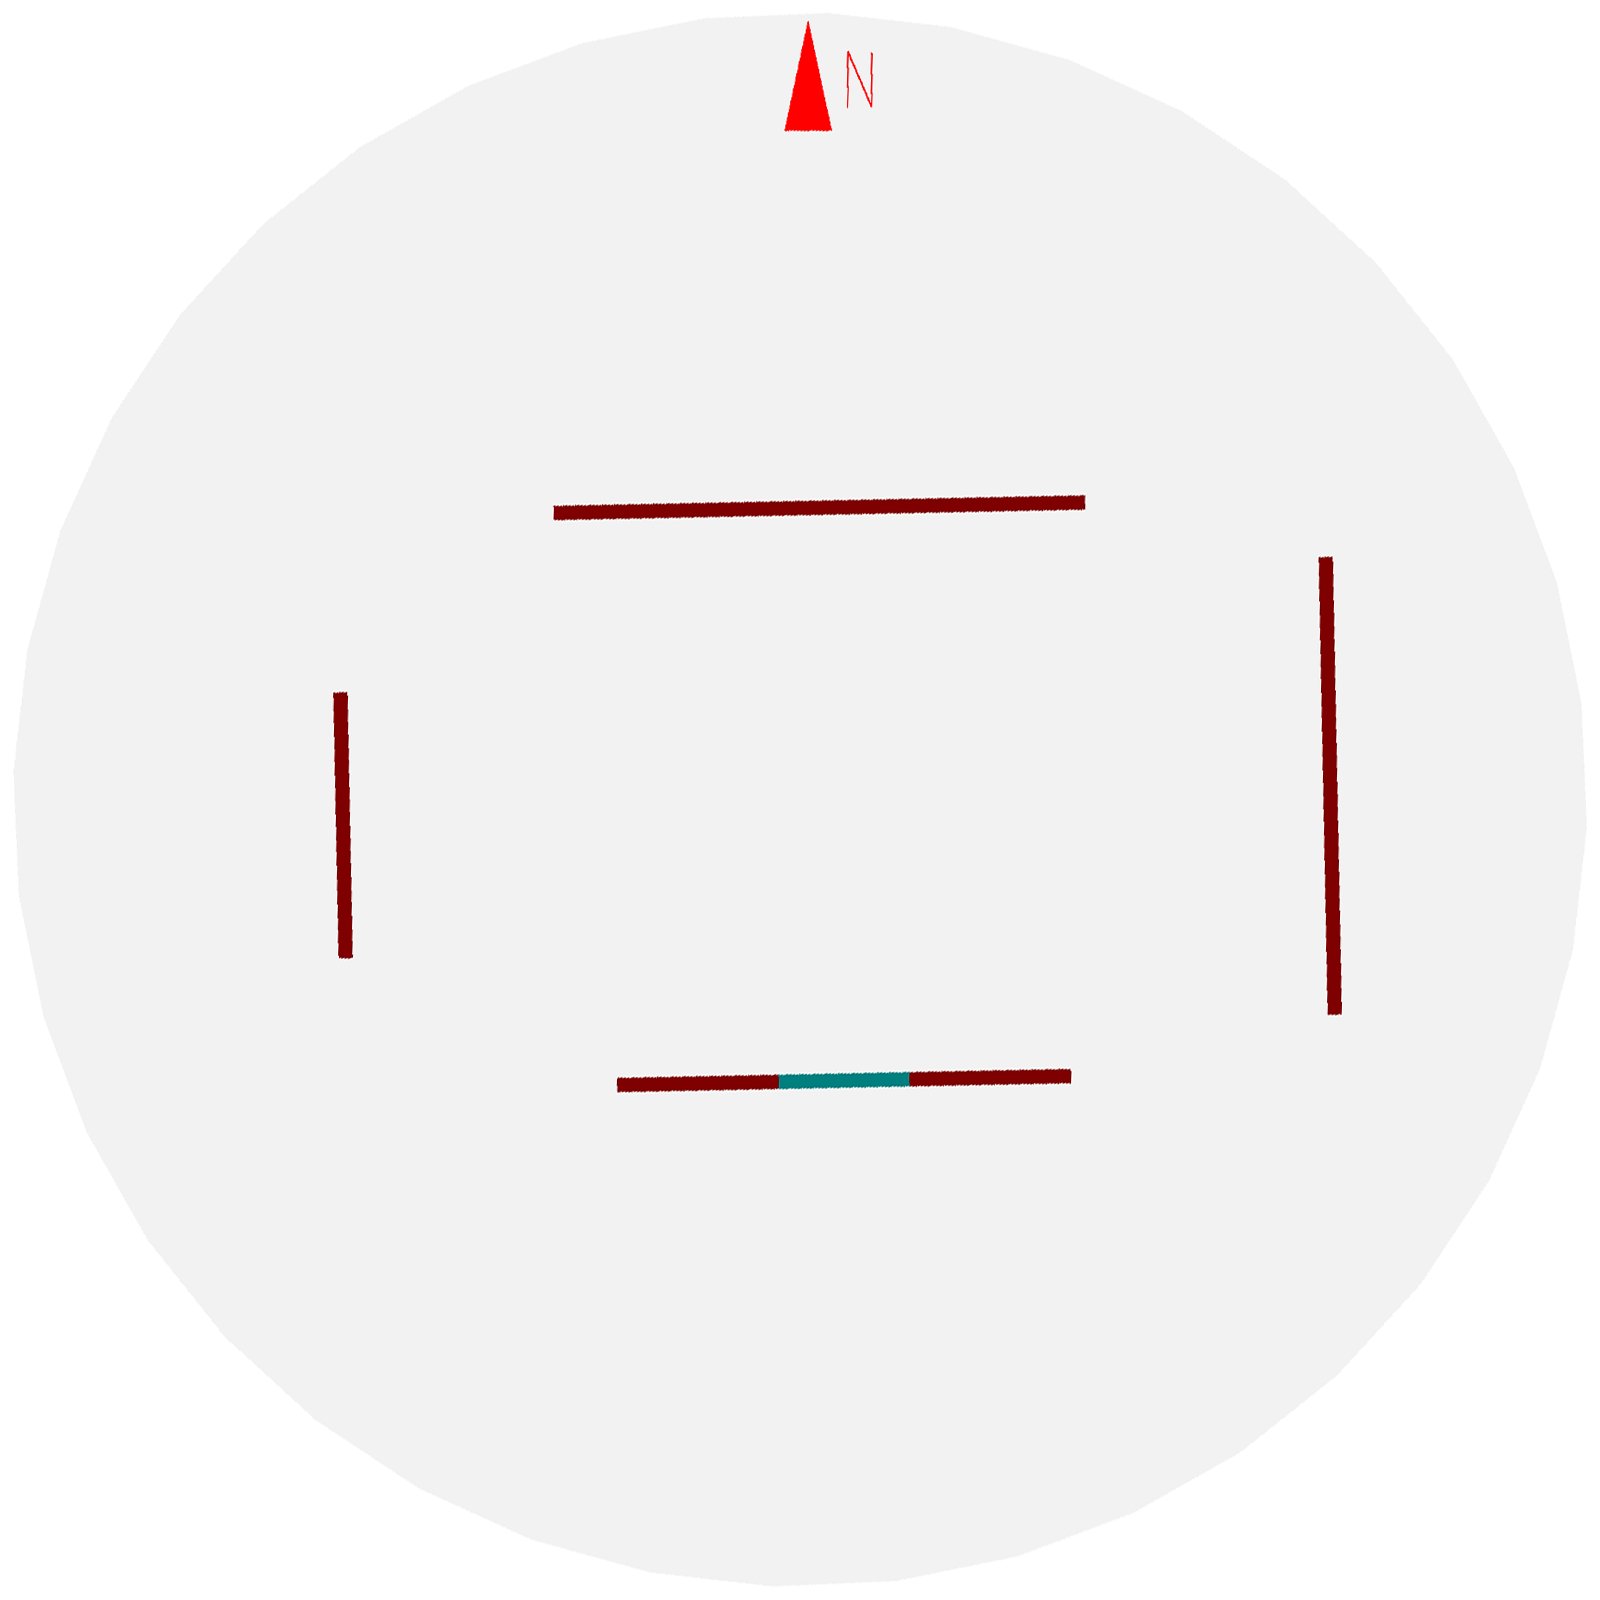
\includegraphics[width=0.7in]{../gi2012_userstudy/images/section2/9_2D_walls_rotate} %N5
  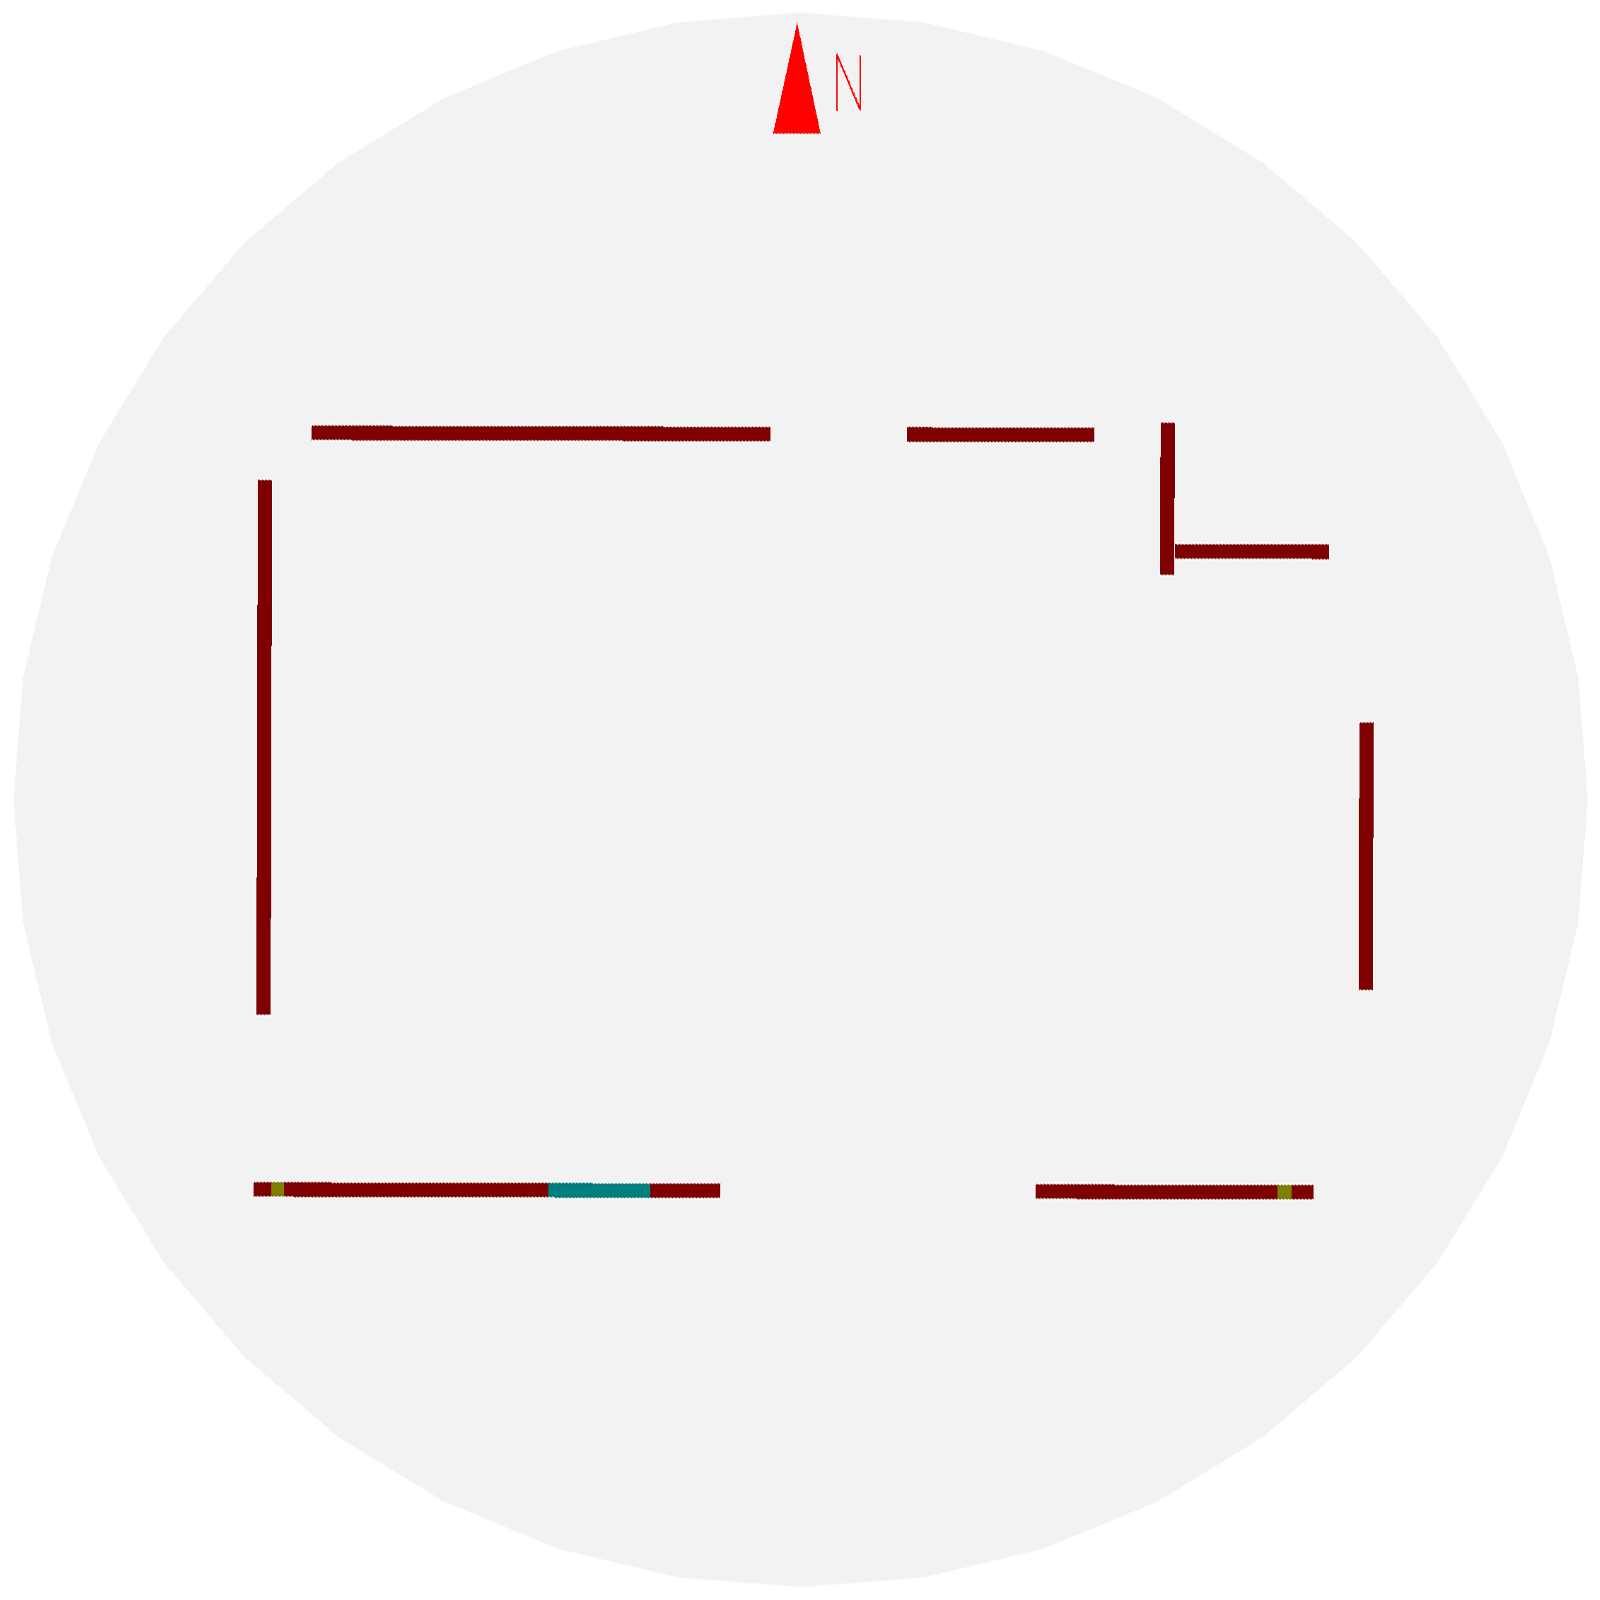
\includegraphics[width=0.7in]{../gi2012_userstudy/images/section2/10_2D_walls_rotate} %N6
  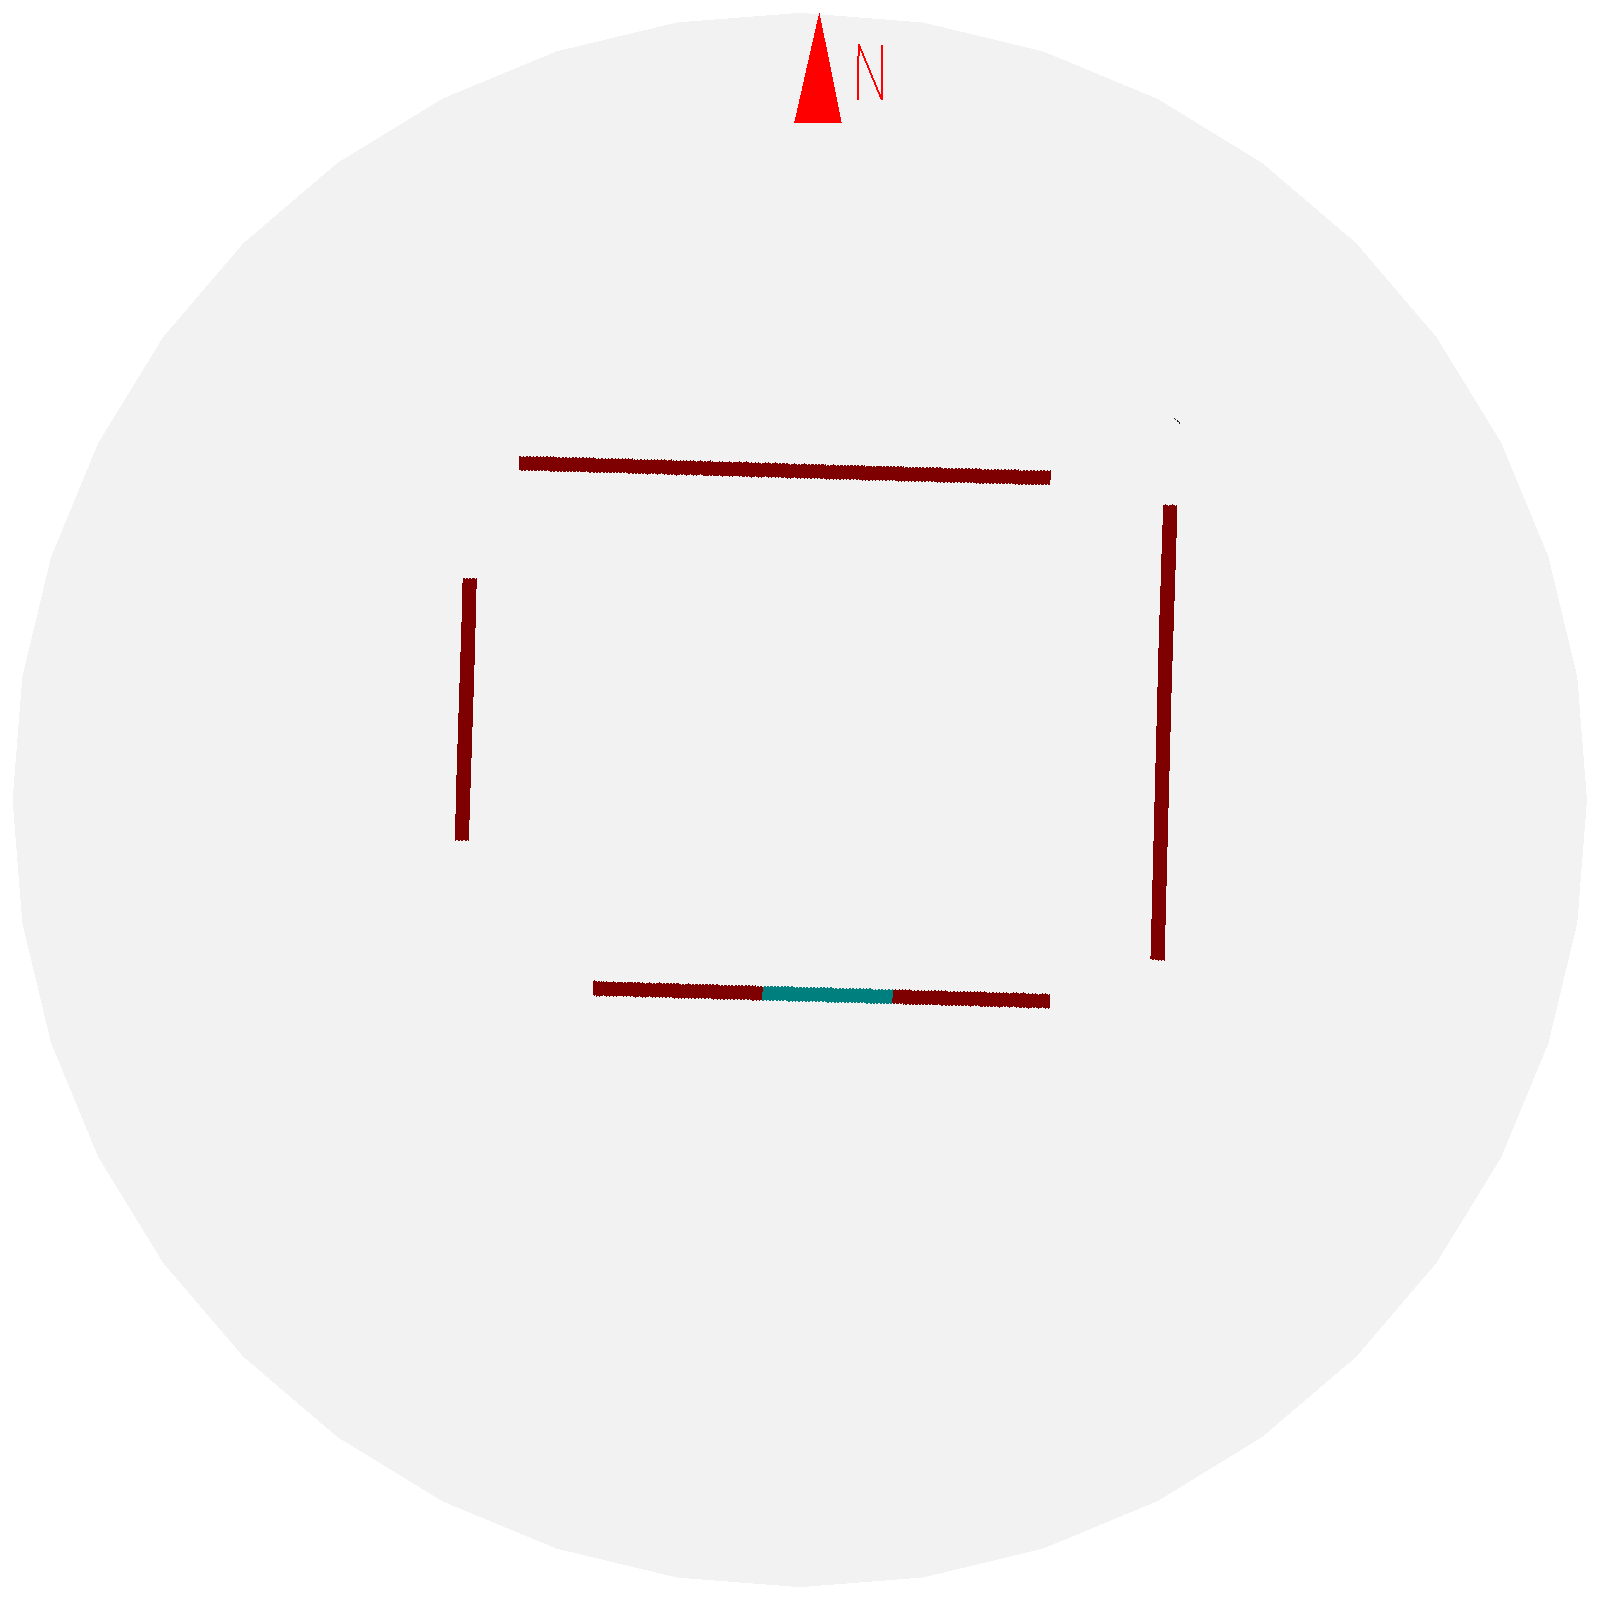
\includegraphics[width=0.7in]{../gi2012_userstudy/images/section2/11_2D_walls_rotate} %N7
\end{minipage}
\vspace{-1.12in}
\\
\begin{minipage}{1.4in}~\end{minipage}
\begin{minipage}{0.7in}{\bf A1}\end{minipage}
\begin{minipage}{0.7in}{\bf A2}\end{minipage}
\begin{minipage}{0.7in}{\bf A4}\end{minipage}
\begin{minipage}{0.7in}{\bf A5}\end{minipage}
\begin{minipage}{0.7in}{\bf A6}\end{minipage}
\vspace{0.78in}
\\
\begin{minipage}{1.4in}{\bf ~N1}\end{minipage}
\begin{minipage}{0.7in}{\bf N2}\end{minipage}
\begin{minipage}{0.7in}{\bf N4}\end{minipage}
\begin{minipage}{0.7in}{\bf N5}\end{minipage}
\begin{minipage}{0.7in}{\bf N6}\end{minipage}
\begin{minipage}{0.7in}{\bf N7}\end{minipage}\vspace{-0.08in}%\\
\end{center}
  \caption{
  \label{figure:original_designs}
A photograph of the physical geometry of the original office space
constructed by one of the participants for Part 2 of the study and 2D
diagrams of the geometry constructed by the other participants.  Note
the variety of model complexity and scale that users create to
represent the same space.  The red walls are 10 inches tall and the
blue walls are 8 inches tall.  Global illumination renderings of these
geometries are shown in
Figure~\ref{figure:renderingsOfOriginalGeometry}.
}
\end{figure*}


\begin{table}[tbp]
\vspace{-0.1in}
\begin{center}
\begin{footnotesize}
\begin{tabular}{@{}l@{~~}|@{~~}r@{~~~}r@{~~~}r@{~~~}r@{~~~}r@{~~}|@{~~}c@{~~~}c@{~~~}c@{~~~}c@{}} 
~       &  {\tiny short}   & {\tiny long}    & {\tiny window}  & {\tiny window} &  {\tiny wall}      &  & & & \\
~       &  {\tiny wall}    & {\tiny wall}     & {\tiny width}   & {\tiny placement} &  {\tiny height}  &  \multicolumn{4}{c}{{\tiny measurement ratios}} \\ 
%How to fit window placement from southwest corner?
~       &  (s)     &  (l)     & (w)     & (p)     &  (h)  &  s:l  &  w:l  &  p:l & s:h \\ \hline
{\tiny ground-truth}  &  24'     &  34'     &  4'     &  10'    &   12'   &\hl{0.71} &\hl{0.12} &\hl{0.29} &\hl{2.00} \\ 
\hline
A1      &  12.0''  &  21.2''  &  3.2''  &  8.8''  &   10''  &  0.57    &  0.15    &  0.41  &  1.20 \\ 
A2      &  14.8''  &  21.2''  &  2.8''  &  6.5''  &   10''  &  0.70    &  0.13    &  0.30  &  1.48 \\ 
A4      &  10.2''  &  15.2''  &  5.1''  &  3.2''  &    8''  &  0.67    &  0.33    &  0.21  &  1.27 \\ 
A5      &  16.2''  &  21.2''  &  3.7''  &  5.5''  &    8''  &  0.76    &  0.17    &  0.26  &  2.02 \\ 
A6      &  12.9''  &  24.5''  &  2.8''  &  7.8''  &    8''  &  0.53    &  0.11    &  0.32  &  1.62 \\ 
N1      &  16.6''  &  23.5''  &  1.8''  &  7.4''  &    8''  &  0.71    &  0.08    &  0.31  &  2.08 \\ 
N2      &  10.2''  &  14.8''  &  1.8''  &  5.1''  &    8''  &  0.69    &  0.13    &  0.34  &  1.27 \\ 
N3      &  12.0''  &  15.7''  &  3.2''  &  5.5''  &    8''  &  0.76    &  0.21    &  0.35  &  1.50 \\ 
N4      &  12.0''  &  19.8''  &  3.2''  &  3.7''  &    8''  &  0.60    &  0.16    &  0.19  &  1.50 \\ 
N5      &  15.7''  &  26.3''  &  3.2''  & 11.5''  &   10''  &  0.60    &  0.12    &  0.44  &  1.57 \\ 
N6      &  20.3''  &  29.5''  &  3.2''  &  7.8''  &   10''  &  0.69    &  0.11    &  0.27  &  2.03 \\ 
N7      &  13.8''  &  18.5''  &  3.2''  &  8.3''  &   10''  &  0.75    &  0.18    &  0.45  &  1.38 \\ \hline  
{\tiny averages } &          &          &         &         &         &          &          &        &\\
{\tiny architects } & 13.2'' & 20.6'' & 3.5''  &  6.4''  &   8.8'' &  \hl{0.64}    &  \hl{0.18}	  &  \hl{0.30}  &  \hl{1.52} \\
{\tiny error  } &     -45\% & -39\% & -12\% & -36\% & -27\% & -9\% & 54\% & 3\% & -24\% \\
{\tiny non-arch. }    & 14.3'' &	21.2'' & 2.8''	&  7.1''  &   8.9'' &  \hl{0.69}    &  \hl{0.14}	  &  \hl{0.34}  &  \hl{1.62} \\
{\tiny error  } &     -40\% & -38\% & -29\% & -29\% & -26\% & -3\% & 19\% & 14\% & -19\%
%13.9''  &  21.0''  &  3.1''  &  6.8''  &  8.8''  &\hl{0.67} &\hl{0.16} &\hl{0.32} &\hl{1.58}\\
\end{tabular}
\end{footnotesize}
\end{center}
\vspace{-0.1in}
\caption{
\label{table:measurements}
The absolute and relative measurements of the
models constructed for Part 2 of the study.
}
\end{table}



\paragraph{Part 3: Analysis of a Proposed Renovation}

The next section exercises the TUI as a design interface with
simulation for analytic support.  The participant is asked to propose
a ``modest'' renovation of the existing space to improve the use of
natural lighting.  This exercise tests if users can effectively and
efficiently make incremental design changes in response to daylighting
needs.  In the spirit of a cognitive walkthrough, few constraints were
placed on the specific edits.  For example, participants could move
and add windows (but only to the exterior wall) and they could add
interior walls.  Once again the users were free to explore their new
design through daylighting simulations of their choosing.  Users were
permitted to further modify their design until satisfied with the
daylighting in the revised model.
%
The short questionnaire at the end of Part 3 asked users to provide
the rational behind their renovation and to estimate the daylight
autonomy of the new space.  
%To better understand the users' experiences,
%a series of questions requesting the users' opinion on the tool's
%ability to help users evaluate illumination, determine the potential
%for glare, understand the qualities of daylighting, and teach
%daylighting concepts.


\paragraph{Part 4: Analysis of a New Design}

The final stage of the study opened the tool to the participants full
creativity.  The user is simply instructed to create a brand new space
with the same program to better serve the needs of same occupants as
the existing lab space.  The new design can be situated anywhere on
campus, in an existing or brand new building.  The participant is
encouraged to request daylighting visualization during the design
process enabling them to creatively experiment with the tool for
uncommonly-shaped spaces.
%
The questionnaire for this section explored the user's motivation
behind the new design, the expressiveness of the physical primitives
for capturing the essential details of the intended design, and the
users estimate of the daylighting autonomy of the new design.  The
intent of Part 4 was both to test if users could freely express an
intended design as well as to see if given complete freedom users were
able to create a space that demonstrated good daylighting
fundamentals.

\begin{figure*}[t]

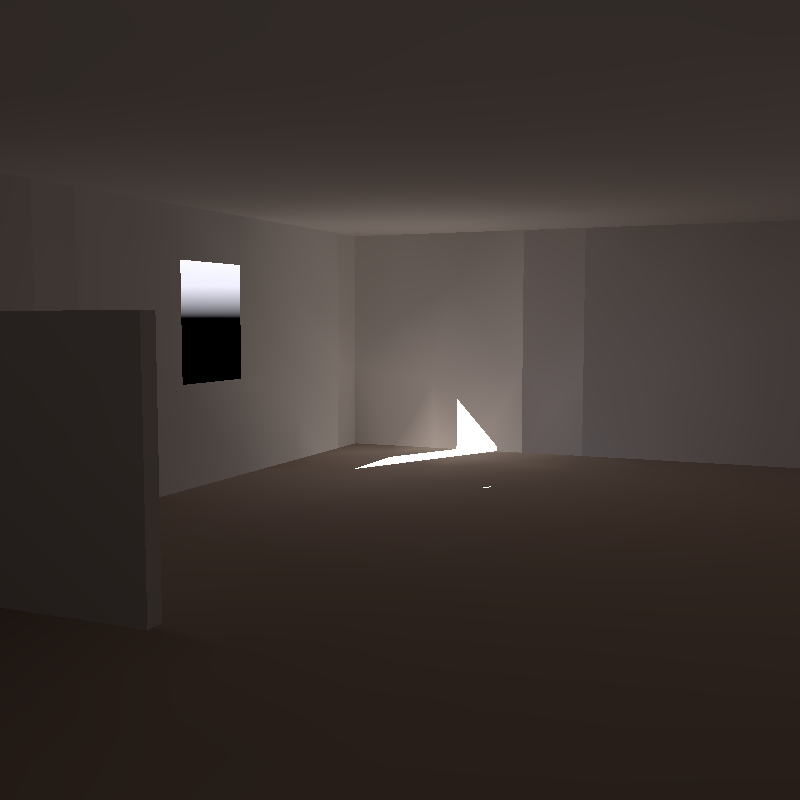
\includegraphics[width=.9in]{../gi2012_userstudy/images/renderings/ground_truth/mrc331_camera_chris_march.png} \hfill  %GT
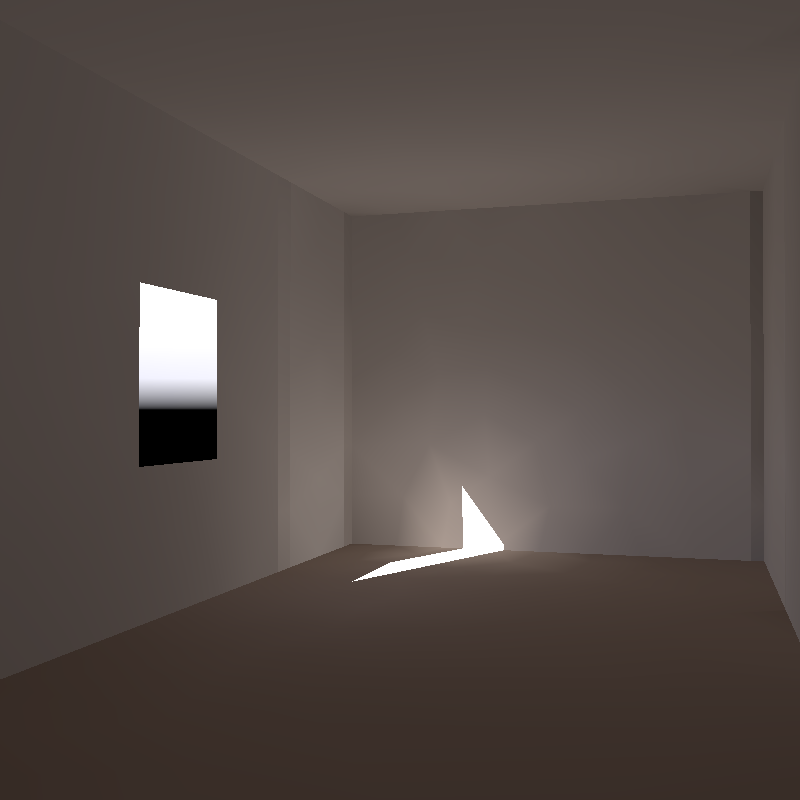
\includegraphics[width=.9in]{../gi2012_userstudy/images/renderings/renovations/065_camera_chris_march.png} \hfill %A1
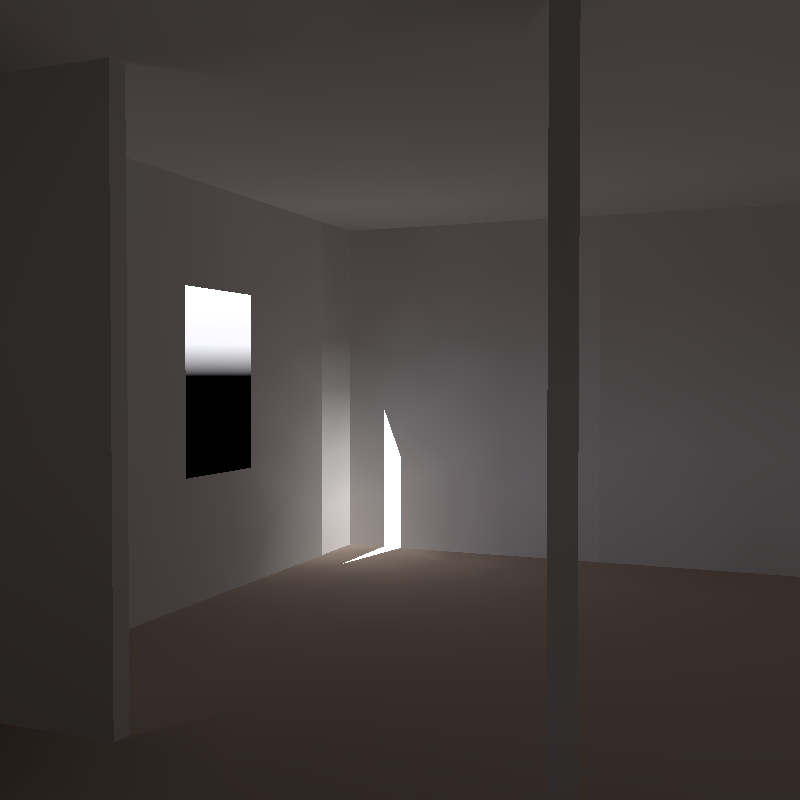
\includegraphics[width=.9in]{../gi2012_userstudy/images/renderings/renovations/038_camera_chris_march.png} \hfill   %A2
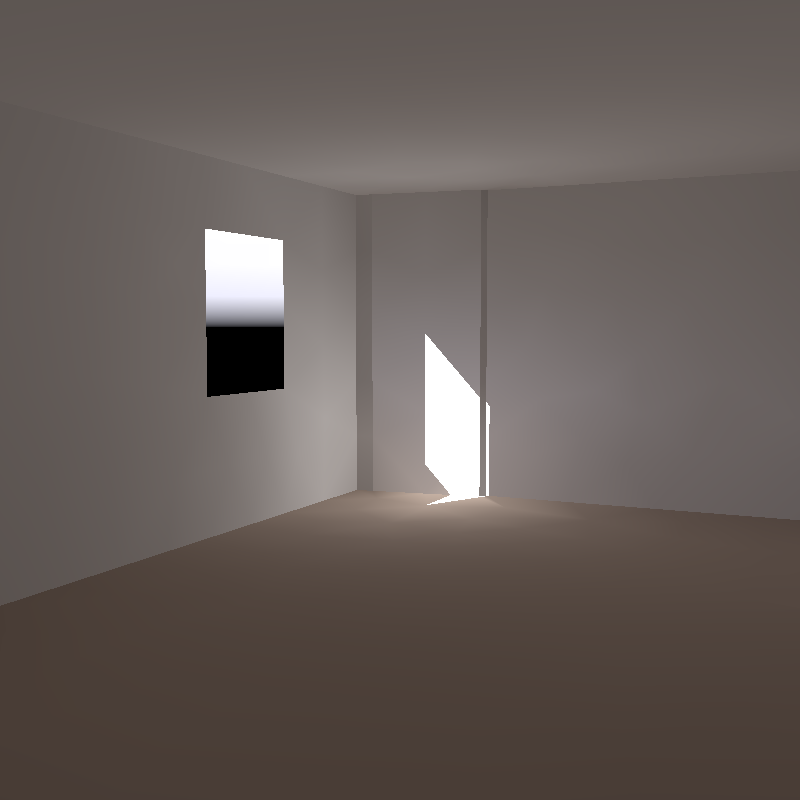
\includegraphics[width=.9in]{../gi2012_userstudy/images/renderings/renovations/042_camera_chris_march.png} \hfill   %A3
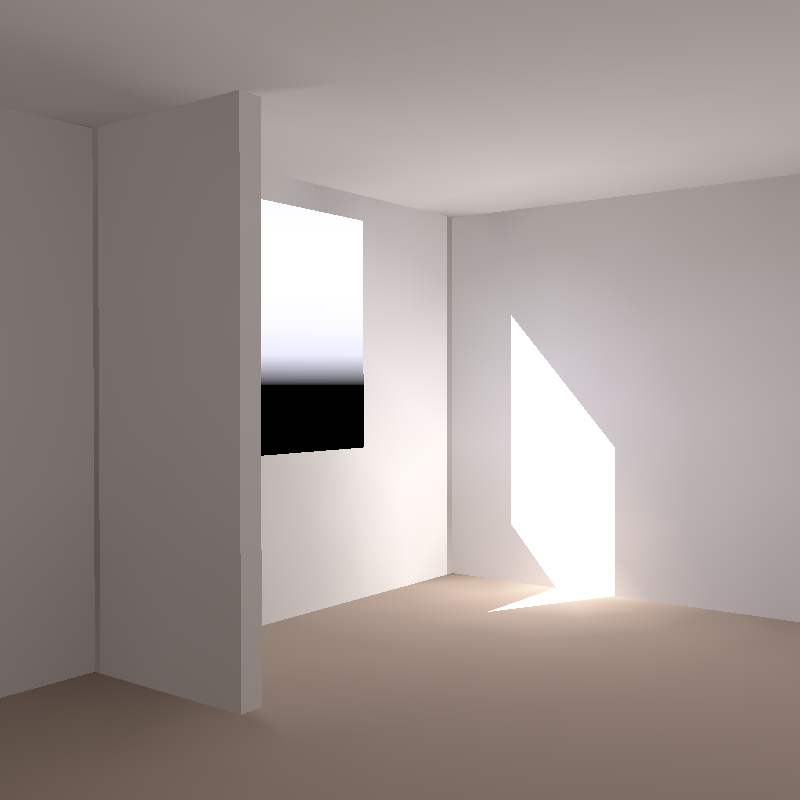
\includegraphics[width=.9in]{../gi2012_userstudy/images/renderings/renovations/031_camera_chris_march.png} \hfill   %A4
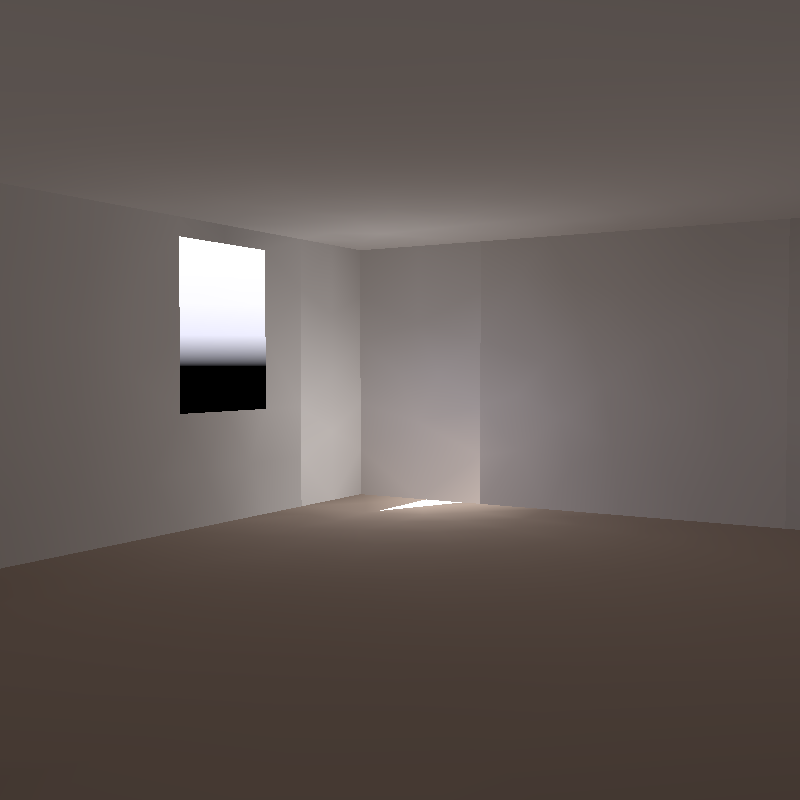
\includegraphics[width=.9in]{../gi2012_userstudy/images/renderings/renovations/014_camera_chris_march.png}\vspace{-0.13in}\\   %A5

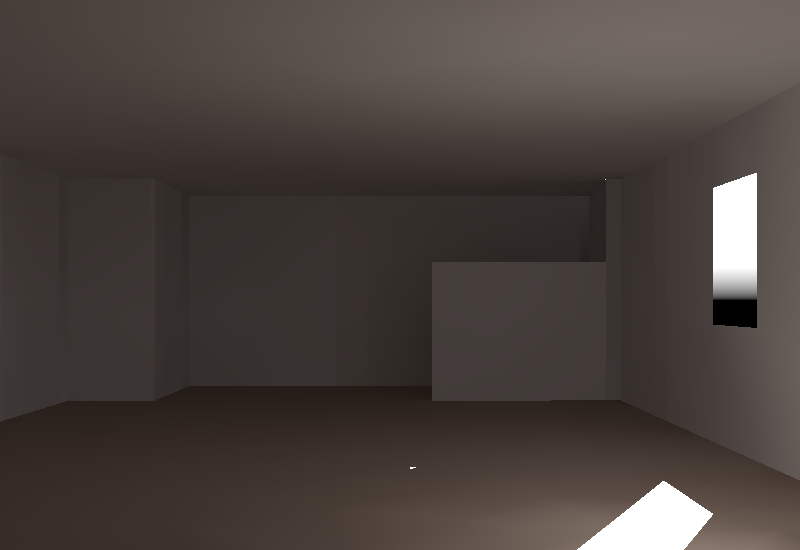
\includegraphics[width=.9in]{../gi2012_userstudy/images/renderings/ground_truth/mrc331_camera_dark_march_crop.png} \hfill %GT
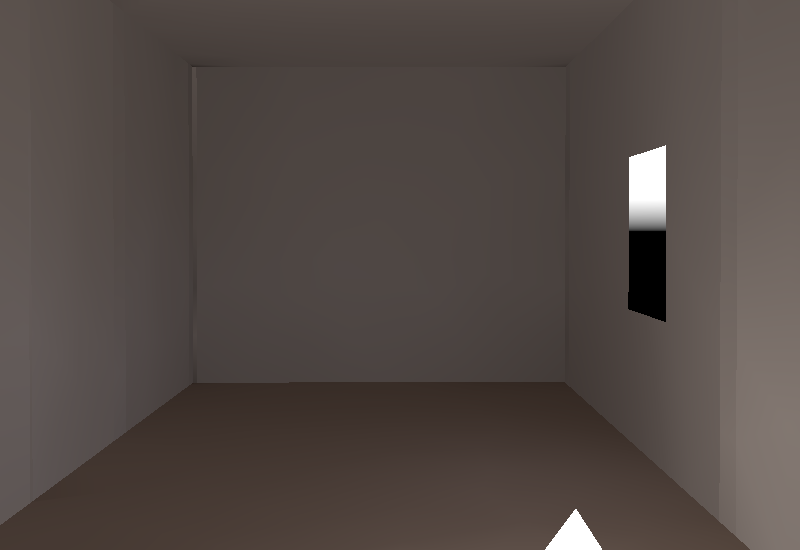
\includegraphics[width=.9in]{../gi2012_userstudy/images/renderings/renovations/065_camera_dark_march_crop.png} \hfill %A1
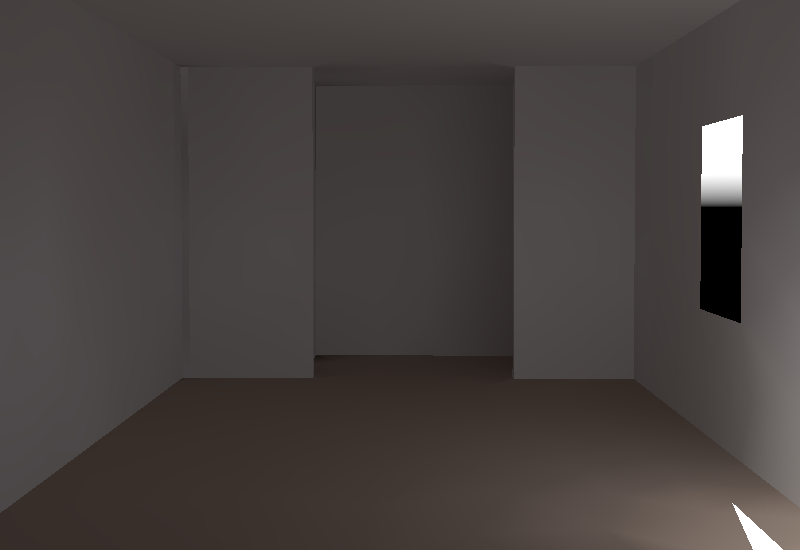
\includegraphics[width=.9in]{../gi2012_userstudy/images/renderings/renovations/038_camera_dark_march_crop.png} \hfill %A2
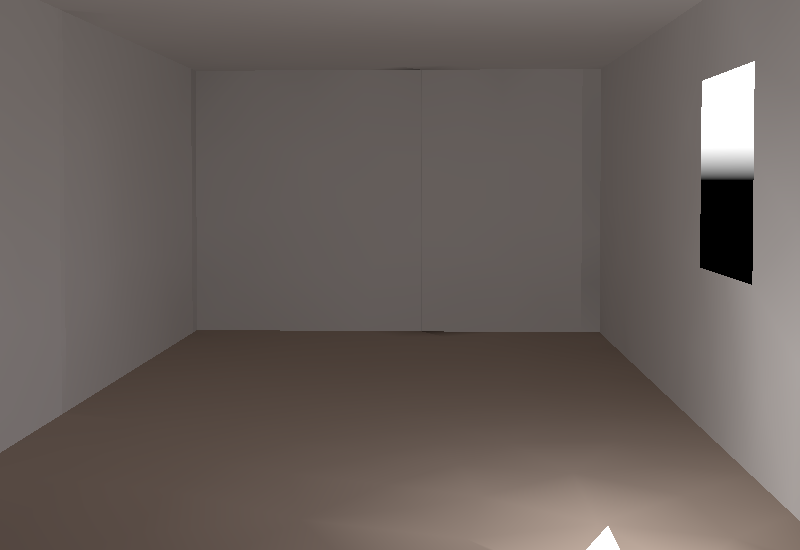
\includegraphics[width=.9in]{../gi2012_userstudy/images/renderings/renovations/042_camera_dark_march_crop.png} \hfill %A3
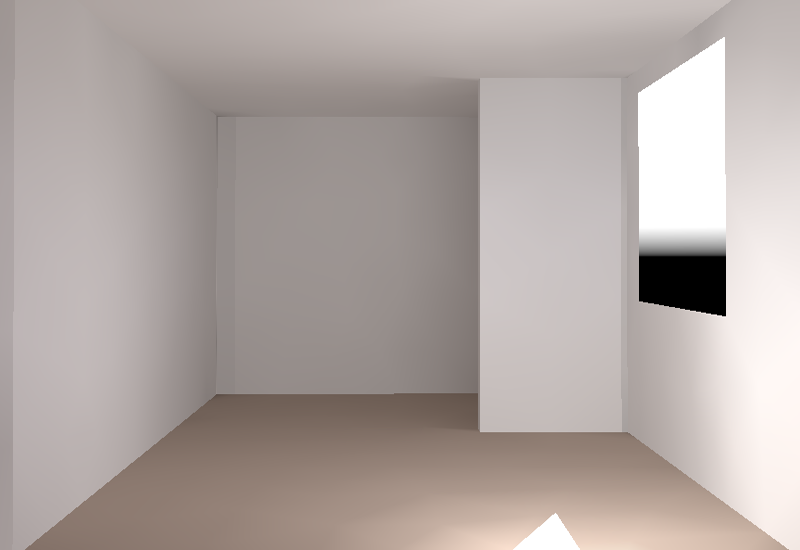
\includegraphics[width=.9in]{../gi2012_userstudy/images/renderings/renovations/031_camera_dark_march_crop.png} \hfill %A4
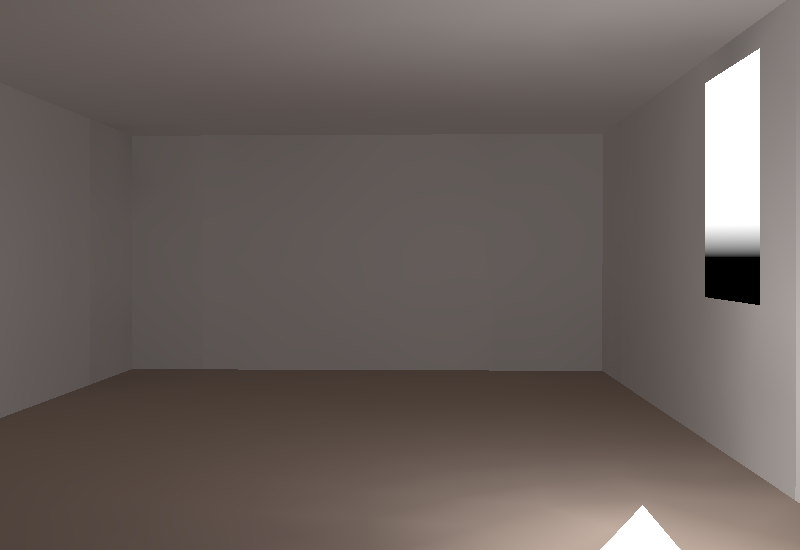
\includegraphics[width=.9in]{../gi2012_userstudy/images/renderings/renovations/014_camera_dark_march_crop.png} \\ %A5

\vspace{-1.84in}
\begin{minipage}{.9in}~{\color{white}{\bf ground-truth}}\end{minipage} \hfill
\begin{minipage}{.9in}~{\color{white}{\bf A1}}\end{minipage} \hfill
\begin{minipage}{.9in}~{\color{white}{\bf A2}}\end{minipage} \hfill
\begin{minipage}{.9in}~{\color{white}{\bf A3}}\end{minipage} \hfill
\begin{minipage}{.9in}~{\color{white}{\bf A4}}\end{minipage} \hfill
\begin{minipage}{.9in}~{\color{white}{\bf A5}}\end{minipage} \\
\vspace{1.47in}

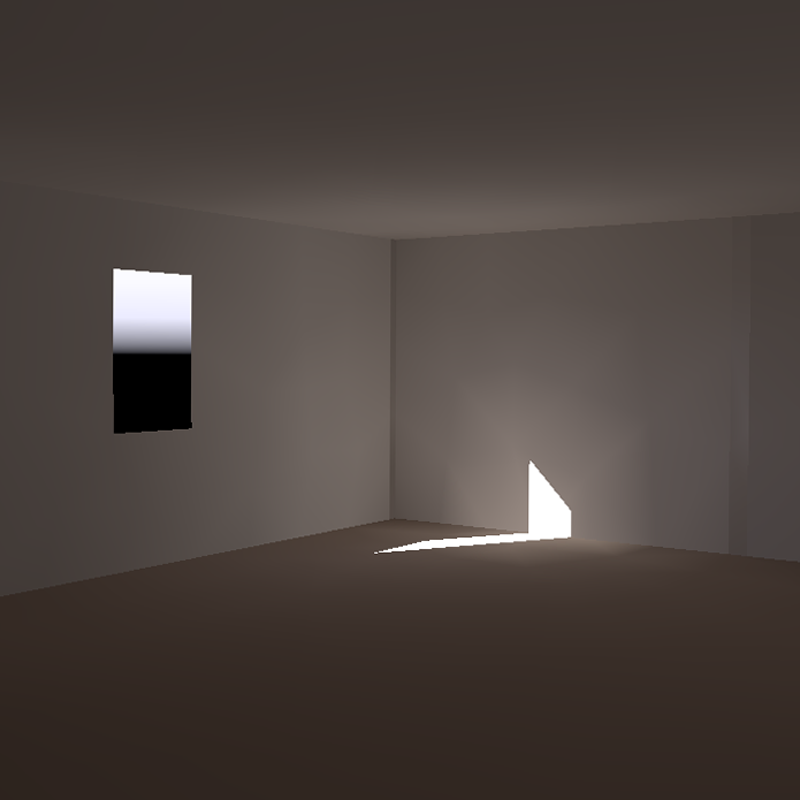
\includegraphics[width=.9in]{../gi2012_userstudy/images/renderings/renovations/063_camera_chris_march_crop.png} \hfill   %N1
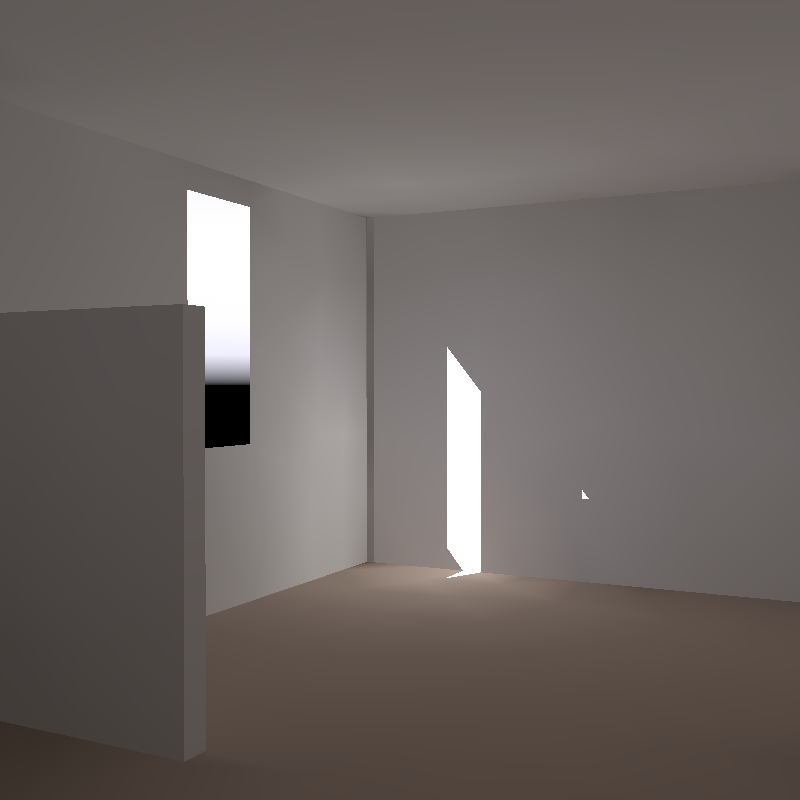
\includegraphics[width=.9in]{../gi2012_userstudy/images/renderings/renovations/050_camera_chris_march.png} \hfill   %N2
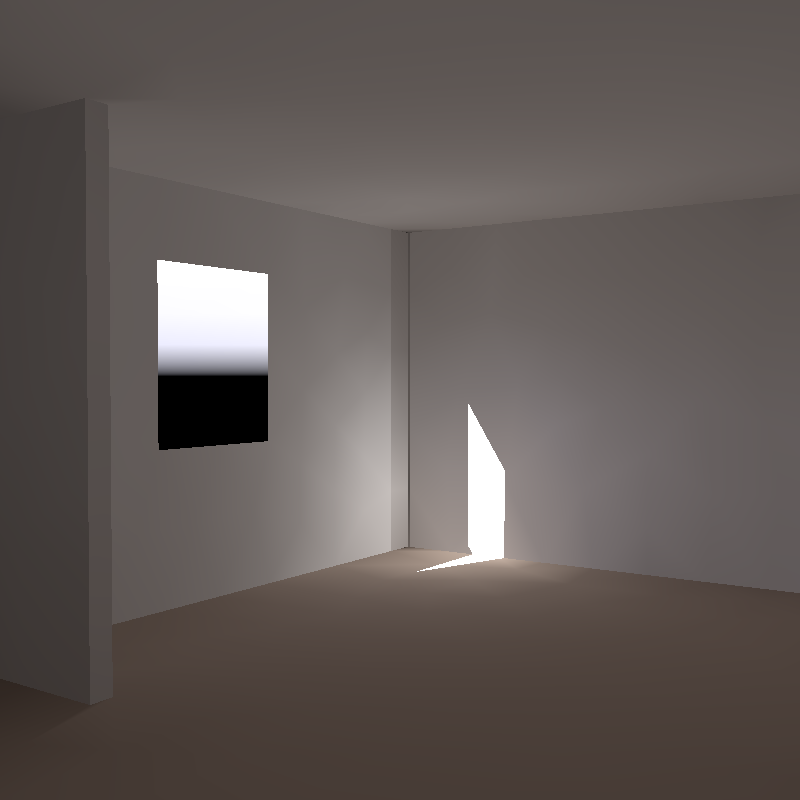
\includegraphics[width=.9in]{../gi2012_userstudy/images/renderings/no_renovations/070_camera_chris_march.png} \hfill        %N3
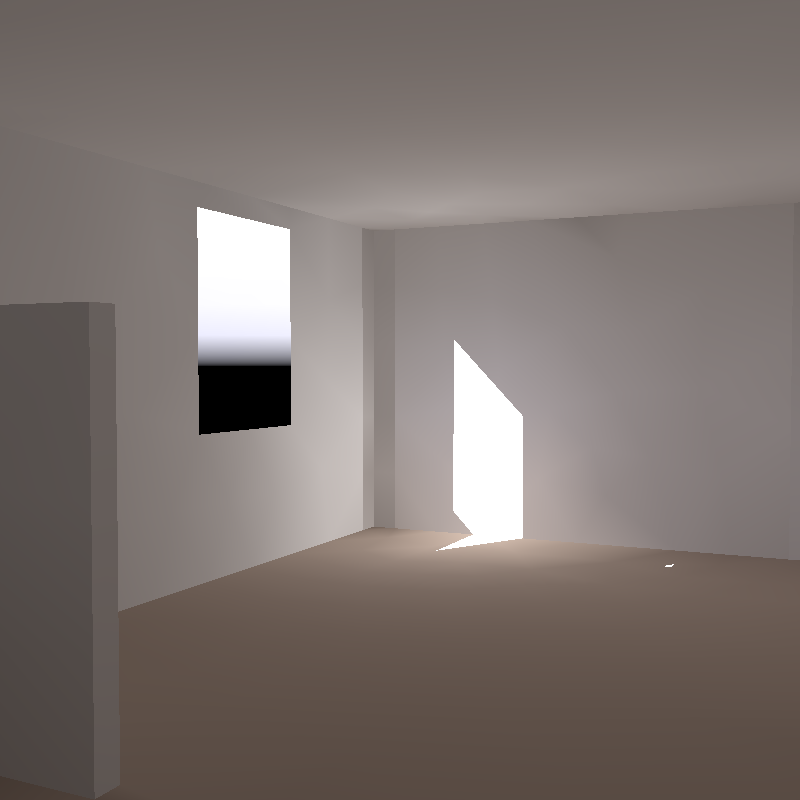
\includegraphics[width=.9in]{../gi2012_userstudy/images/renderings/renovations/098_camera_chris_march.png} \hfill   %N4
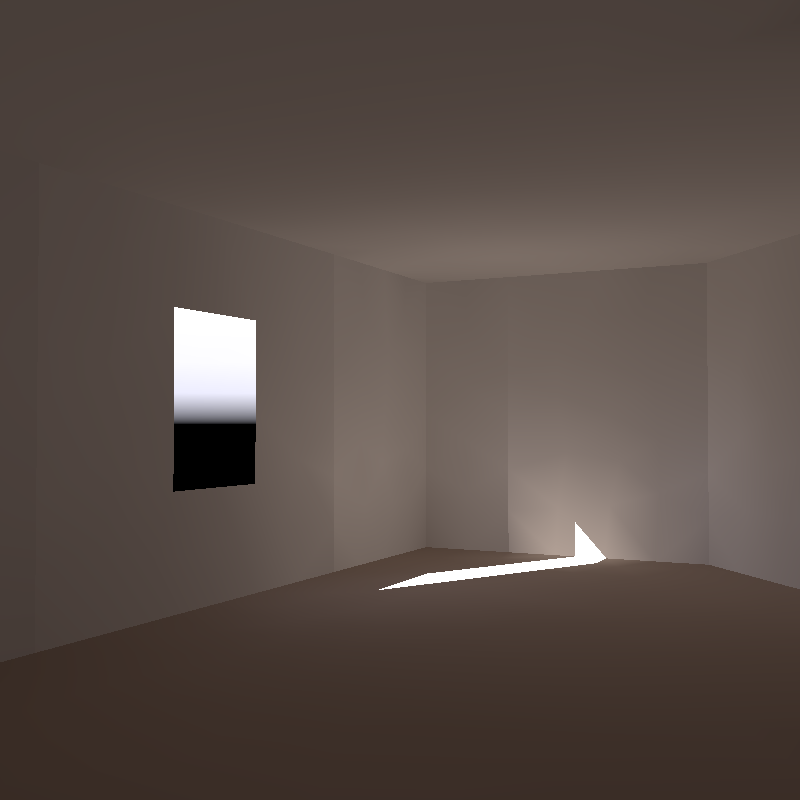
\includegraphics[width=.9in]{../gi2012_userstudy/images/renderings/no_renovations/user_085_camera_chris_march.png} \hfill   %N5
%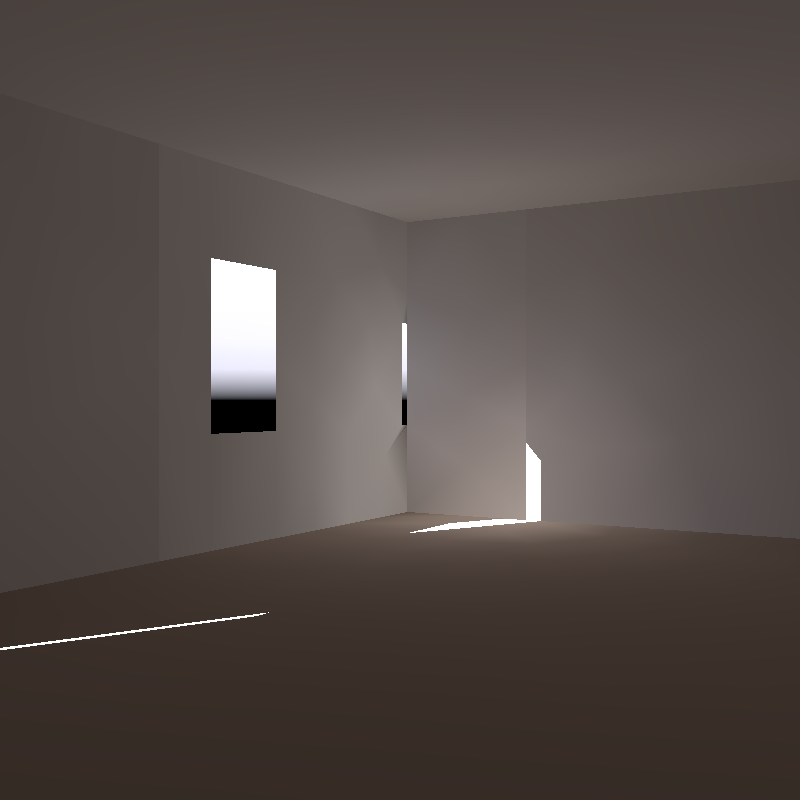
\includegraphics[width=1.1in]{../gi2012_userstudy/images/renderings/renovations/user_046_camera_chris_march.png}\vspace{-0.13in}\\   %N6
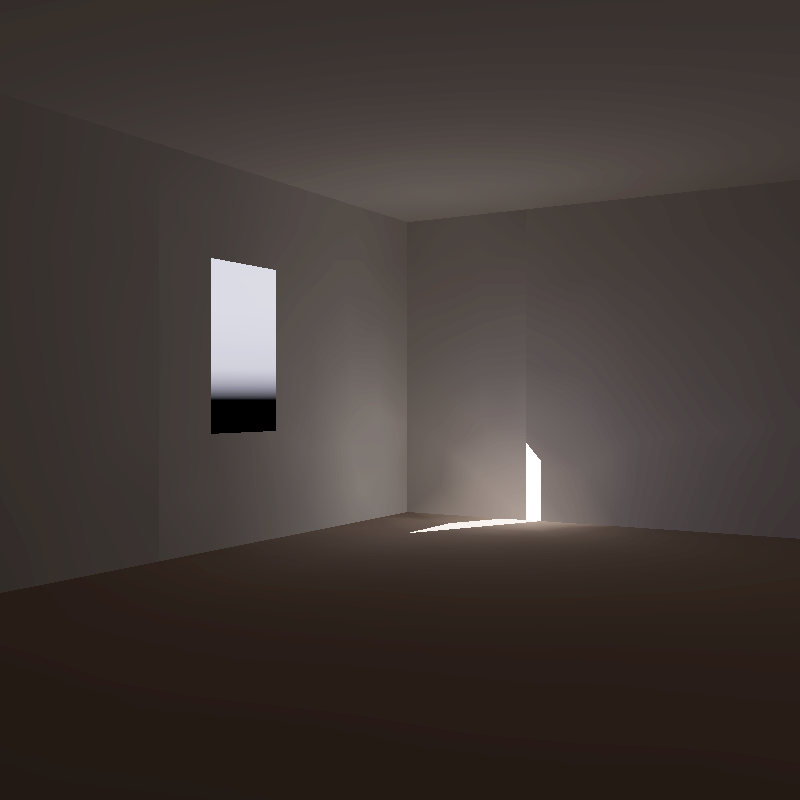
\includegraphics[width=.9in]{../uist2012/images/renovations/PRE_N6_march_chris.png}\vspace{-0.13in}\\ 

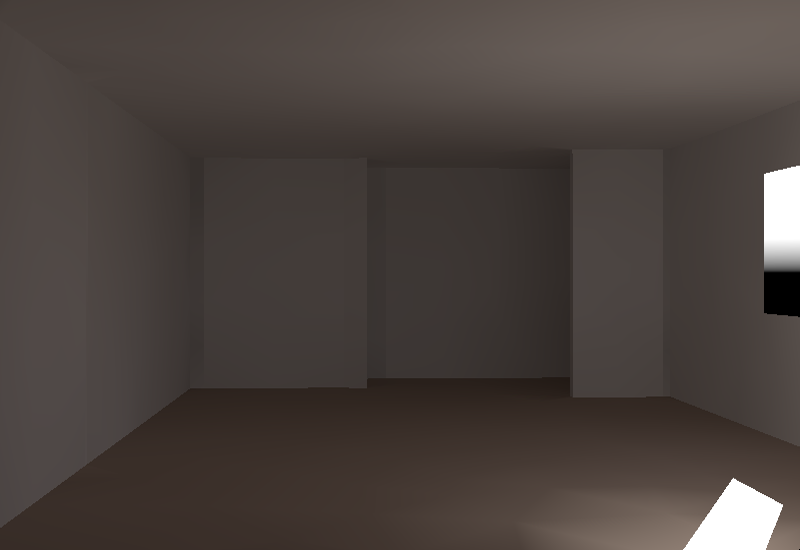
\includegraphics[width=.9in]{../gi2012_userstudy/images/renderings/renovations/063_camera_dark_march_crop.png} \hfill    %N1
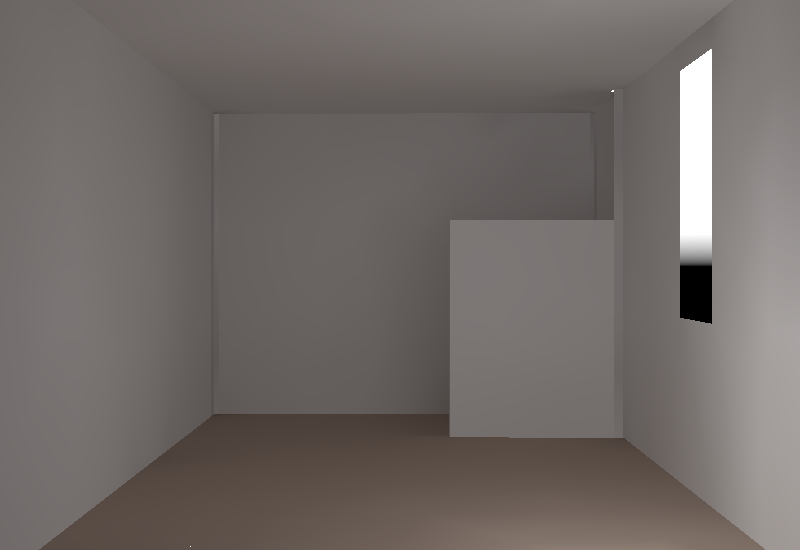
\includegraphics[width=.9in]{../gi2012_userstudy/images/renderings/renovations/050_camera_dark_march_crop.png} \hfill    %N2 BARB
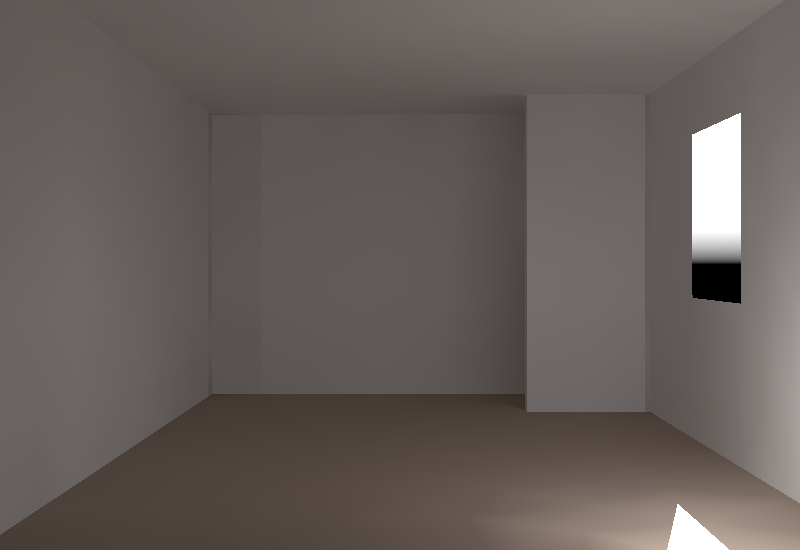
\includegraphics[width=.9in]{../gi2012_userstudy/images/renderings/no_renovations/070_camera_dark_march_crop.png} \hfill         %N3
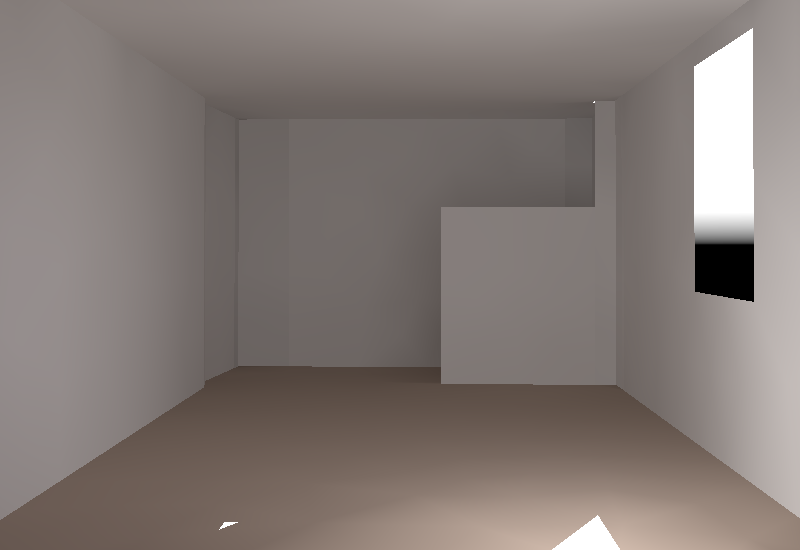
\includegraphics[width=.9in]{../gi2012_userstudy/images/renderings/renovations/098_camera_dark_march_crop.png} \hfill    %N4
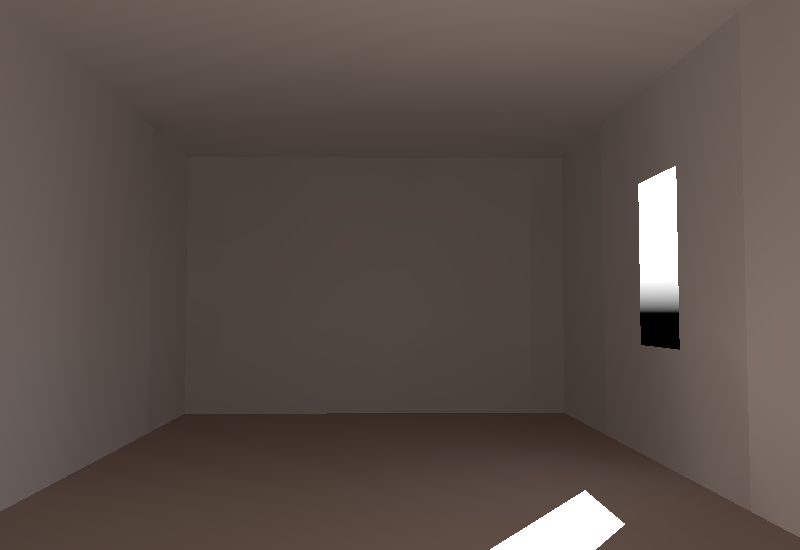
\includegraphics[width=.9in]{../gi2012_userstudy/images/renderings/no_renovations/user_085_camera_dark_march_crop.png} \hfill    %N5
%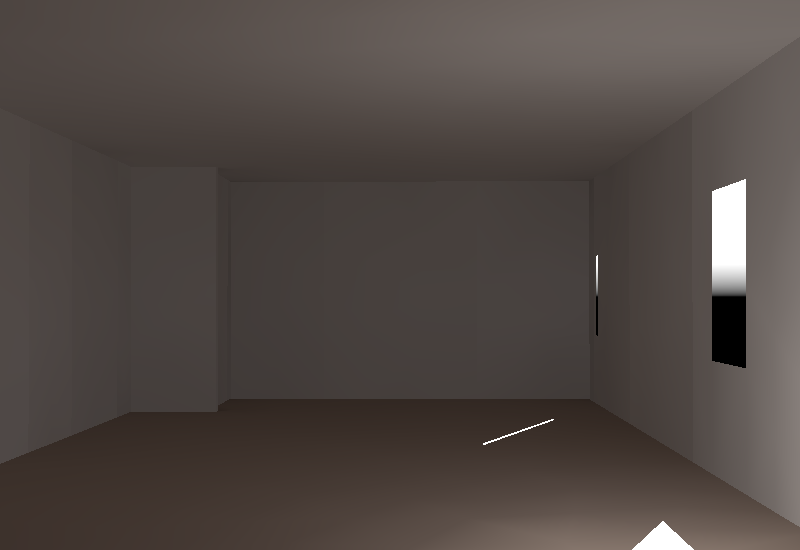
\includegraphics[width=1.1in]{../gi2012_userstudy/images/renderings/renovations/user_046_camera_dark_march_crop.png} \\   %N6
\includegraphics[width=.9in]{../uist2012/images/renovations/PRE_N6_march_dark.png} \\

\vspace{-1.84in}
\begin{minipage}{.9in}~{\color{white}{\bf N1}}\end{minipage} \hfill
\begin{minipage}{.9in}~{\color{white}{\bf N2}}\end{minipage} \hfill
\begin{minipage}{.9in}~{\color{white}{\bf N3}}\end{minipage} \hfill
\begin{minipage}{.9in}~{\color{white}{\bf N4}}\end{minipage} \hfill
\begin{minipage}{.9in}~{\color{white}{\bf N5}}\end{minipage} \hfill
\begin{minipage}{.9in}~{\color{white}{\bf N6}}\end{minipage}
\vspace{1.47in}

\caption{ Simulation results for the original room geometry
  constructed by the study participants shown in
  Figure~\ref{figure:original_designs}.  The ground-truth model was
  constructed with the same tangible interface using the true room
  dimensions.  All models are constructed using the same floor, wall,
  and ceiling materials.  All renderings in this figure are March 21st
  at 8:30am.  The desks in the southwest corner of the room (1st and
  3rd rows) experiences glare at this time.  The east side of the room
  (2nd and 4th rows) is quite dark all year, especially in the
  mornings.  }
\vspace{-0.1in}
\label{figure:renderingsOfOriginalGeometry}
\end{figure*}


\subsection{User Study Results}

Users demonstrated different styles of design, both in modeling and in
daylighting analysis strategy.  Architects and non-architects alike
entered the study with varying levels of daylighting intuition to the
study.

\paragraph{Part 1: Intuition of Existing Design}

An important concept in understanding and evaluating daylighting is
the sun's height and track across the sky for different seasons.  The
two extremes happen on the solstices.  In the northern hemisphere, the
sun reaches the highest point in the sky (angle to the horizon) during
the summer solstice (June 21).  The winter solstice (December 21) is
the day the sun reaches the lowest point in the sky at mid-day.  March
21 and September 21 are the equinoxes.  The sun's track from east to
west across the sky, goes across the southern sky.  This means that
most direct light in buildings is obtained from south facing windows.
Furthermore, direct sunlight will reach much further into a space from
a southern facing window in the winter.
%
From experience, we know that the case study computer lab
(Figure~\ref{figure:example_room}) has some very specific lighting issues.
The desk closest to the window has significant over-illumination as
well as glare issues for the morning hours, which are especially
problematic in the winter.  The far side of the room is consistently
under-illuminated.  The desks in the center of the room suffer from
substantial glare issues, those facing away from the window suffer
from glare on the monitors, while the ones facing towards the window
have glare because the window is so much brighter than the monitors.
The east (left) side of the room suffers consistently from
under-illumination because of its distance from the window.  We
compare this knowledge with the analysis done by the users concerning
the lighting in the space.

The users' sketches varied in level of detail and style
(Figure~\ref{figure:sketches}), but users consistently identified
areas of too much and too little daylighting in the room.  Users did
the study at a variety of times in a variety of weather conditions
(cloudy/sunny, morning/afternoon, etc.), but their results showed no
noticeable relation to these conditions.  Five out of six of the
architects identified a cone shaped area of bright light near the
window.  All of the architects used a 2D {\em plan} view to convey
their information.  However, the architects were not consistent in
where they identified problematic areas for glare.  Three of the
architects discerned the desks in the center of the room would have
problem with glare.  Most users recognized that the desks near the
window would be very bright, but only three of the architects
recognized glare being a problem in this area.  Architects in general
demonstrated a clear understanding 
%seem to have a pretty good idea
%\fbox{ Language too informal here?}
of the approximate area lit by a
window, but have difficulties discerning how bad glare will be and
when it will be a problem.  One architect claimed the worst
over-illumination would occur in the summer.  This intuition was
exactly opposite of the true lighting condition at midday.

The style of the non-architects' drawings were more varied. Two of the
seven used 3D perspective to sketch the room.  The non-architects did
not specifically identify a cone-shaped area of over-illumination near
the window but did provide appropriate detail of problematic lighting
areas.  Their intuition about lighting concepts also seemed to be of a
similar depth and accuracy.  In fact, one user from each category
(architect and non-architect) demonstrated correct intuition in which
areas would be problems at various points throughout a given day
%While this is a fairly small sample size, it appears that these
%particular architecture students' training (at least in the first two
%years) has not focused on  about daylighting is not farmay be fairly limited.

\begin{figure*}[t]
\begin{minipage}[c]{0.49\textwidth}
  \includegraphics[width=0.49\textwidth]{p3m_38_renovation_flipped_northarrow} %A2
  \includegraphics[width=0.49\textwidth]{p3m_42_renovation} %A3
\end{minipage}
\begin{minipage}[c]{0.5\textwidth}
  \includegraphics[width=0.24\textwidth]{p3m_0_2D_walls_rotate_edit} %A1
  \includegraphics[width=0.24\textwidth]{p3m_6_2D_walls_rotate} %A4
  \includegraphics[width=0.24\textwidth]{p3m_7_2D_walls_rotate} %A5
  \includegraphics[width=0.24\textwidth]{p3m_8_2D_walls_rotate}\\ %A6
  \includegraphics[width=0.24\textwidth]{p3m_2_2D_walls_rotate} %N2
  \includegraphics[width=0.24\textwidth]{p3m_3_2D_walls_rotate} %N3
  \includegraphics[width=0.24\textwidth]{p3m_4_2D_walls_rotate} %N4
  \includegraphics[width=0.24\textwidth]{p3m_9_2D_walls_rotate} %N6
\end{minipage}
\vspace{-0.175\textwidth}
\\
\begin{small}
\begin{minipage}{0.245\textwidth}~\end{minipage}
\begin{minipage}{0.245\textwidth}~\end{minipage}
\begin{minipage}{0.117\textwidth}{\bf A1}\end{minipage}
\begin{minipage}{0.117\textwidth}{\bf A4}\end{minipage}
\begin{minipage}{0.117\textwidth}{\bf A5}\end{minipage}
\begin{minipage}{0.117\textwidth}{\bf A6}\end{minipage}%
\vspace{0.09\textwidth}
\\
\begin{minipage}{0.245\textwidth}{\bf ~A2}\end{minipage}
\begin{minipage}{0.245\textwidth}{\bf ~A3}\end{minipage}
\begin{minipage}{0.117\textwidth}{\bf N2}\end{minipage}
\begin{minipage}{0.117\textwidth}{\bf N3}\end{minipage}
\begin{minipage}{0.117\textwidth}{\bf N4}\end{minipage}
\begin{minipage}{0.117\textwidth}{\bf N6}\end{minipage}\vspace{0.0in}%
\end{small}
  \caption{ In Part 3 of the study participants were asked to propose
    a modest renovation to the geometry to improve the use of
    daylighting.
%Three users came up with especially creative ways to deal with glare in the space.
Renderings of several of these geometries are shown
in
%Figures~\ref{figure:renovations}.
Figures~\ref{figure:brighter_renovations}~and~\ref{figure:diffusing_renovations}.
\label{figure:improved_designs}
  }

\vspace{-0.1in}
\end{figure*}



\paragraph{Part 2: Analysis of Existing Design}

First we evaluate the accuracy of the model construction.
Table~\ref{table:measurements} presents a detailed comparison of the
absolute and relative dimensions of the models built by the
participants (Figure~\ref{figure:original_designs}).
%
Users were provided with the rough measurements of the lab (24' x 34'
and 10' tall) at the beginning of the study.  The suggested scale for
the physical sketching environment is 1/12 scale (so 1' in the real
world would be 1'' in the model) and the participants are told that
the blue edged walls are 8'' tall, the red edges walls are 10'', and
the small green walls are 5'' tall.
%
While eight out of thirteen users made a 8'' tall model, this fact is
not significant because the propagation of light is the same at
different scales.  Furthermore, several users specifically selected
the smaller scale because there were more total 8'' primitives than
10'' primitives.
%\fbox{Do you want to mention that? It doesn't seem to add anything}
%While eight out of thirteen users made a 8 inch tall model, we decided
%it was not significant because multiple users requested to use a
%slightly different scale due to there being more 8 inch primitives
%available than 10 inch primitives. Note that size does not matter as
%light will interact the same on different scales.
%

Overall, users were relatively accurate (within 15\%) with the
dimensions of the outer walls and with the placement of the window on
the wall.  Users were less accurate in the ratio of the height to
wall, which does have significant impact on daylighting.  
%Because the
%windows are proportional to the height of the wall in our program,
%this has a direct affect on the amount of light in the room.  
This error was skewed to creating models that were taller than the
ground truth, allowing more light 
% CHRIS
to reach
 into the far corners of the
room.  
%The 24\% misestimation of the architects and the 19\% error of the
%non-architects will result in simulations that are noticeably brighter
%or darker than the ground truth.
%
Users were surprisingly inaccurate with the length of the window in
relation to the size of the wall.  The window width error was skewed
to create models with windows that were too big, resulting in
simulations that are noticeably brighter than the ground truth.
%Non-architects overestimated the
%size by 19\% whereas architects overestimated the size by 54\% (only
%21\% if the worst outlier is removed).  
%While users seem to have compensated their errors on the width of the
%window with the height of the wall, 
It is notable that many users did not 
more 
carefully observe and
reproduce the dimensions of the window.  
%Also, because the window
%appeared to often be the wrong shape, the lighting will less accurate.
%
Global illumination renderings of the geometry created in Part 2 of
the study are presented in
Figure~\ref{figure:renderingsOfOriginalGeometry}.  All models
correctly capture the problem with glare in the southwest corner of
the room in the morning.  However, the variation in brightness and
distribution of light within the space, compared to the ground truth,
does indicate the relative importance and negative impact of geometric
errors in the modeling process.


As this was the users' first experience with the TUI daylighting tool,
most users requested 5-10 different daylighting simulations.  Most
users chose to view a winter date, a summer date, and one or both of
the fall and spring equinoxes.  Two architects and two non-architects
chose the solstices within a couple days.  Others mostly chose dates
across the seasons.  All users recognized the importance of requesting
multiple dates throughout the year.  Some users were familiar with the
seasonal patterns while others demonstrated incorrect initial
intuition: e.g., two architects expressed confusion between the
equinoxes and the solstices.  After daylighting exploration with the
tool, most users solidified a correct understanding of seasonal
daylight patterns, although at least one user, A6, failed to grasp
this concept.  In Part 2, many users appreciated the complex
visualization the tool provided, allowing them to better evaluate
parts of the room that had significant glare.  Although users still
had a large range (30\% to 90\%) in their opinions of the daylight
autonomy users only changed their original estimations by an average
%bsolute value of 
20\% from their original estimate.  
%Overall users impression
%of daylighting in this space were positively influenced by the TUI.
%use of
%the tool, even though their perceptions of lighting still varied
%widely.


On the questionnaire participants were asked: ``What new insights did
you gain about daylighting within the space?  Were any of the
simulation results unexpected?''
%
5 out of 6 architects and 6 out of 7 non-architects claimed they
gained additional daylighting insight from this first task.  A1 said
``I learned there was much more light shed on the west wall than I
expected, and was less light on the north and east walls, especially
on the north."  User A2 was surprised by the sun's penetration into
the room: ``New insights would be that the room's depth is rather
shallow in the winter months when the sun is low, allowing the light
to cause a significant amount of glare all the way across the room."
Not only did users find areas of problematic lighting but users who
requested the most simulations also were able to identify problematic
times.  Participant A5 said ``I learned how the sun's direction
relative to the date and time is a huge factor . . .''
% since I also saw March
%20 from noon to 6 PM to see the difference.'' 
%Interestingly, 
Some users credited the tool with reminding them
of key
%helped them remember things about
daylighting properties:
%which they hadn't remembered correctly when evaluating
%without the tool: 
``I forgot to take into account that during the
summer the sun is higher up, so actually less light penetrates
throughout the room.''  Non-architects remarked on what they learned
as well, but most of them offered more generic remarks.  N6 commented:
``I gained additional insight into how the lighting changes throughout
the day, and at different times in the year.  I was then able to
compare them with each other to see the tendencies of the lighting in
the room.''
%
Despite some inaccuracies in model dimension and scale, participants
gained quite a bit of insight about the daylighting in the case study
space with the TUI. 
% Architects gained specific insights into where
%light would fall in the space; non-architects seemed to gain more
%general knowledge about the dynamic nature of daylighting.



%\begin{comment}

\begin{figure*}[t]
\newcommand{\figwidth}{0.155\textwidth}
\includegraphics[width=\figwidth]{p3r_065_camera_chris_march.png} %A1
\includegraphics[width=\figwidth]{p3r_065_camera_chris_march_mod.png} %A1
\hfill
\includegraphics[width=\figwidth]{p3r_031_camera_chris_march.png}   %A4
\includegraphics[width=\figwidth]{p3r_031_camera_chris_march_mod.png}   %A4
\hfill
\includegraphics[width=\figwidth]{p3r_063_camera_chris_march.png}   %N1
\includegraphics[width=\figwidth]{p3r_063-2_camera_chris_march_mod.png}   %N1

\includegraphics[width=\figwidth]{p3r_065_camera_dark_december_crop.png} %A1
\includegraphics[width=\figwidth]{p3r_065_camera_dark_december_mod_crop.png} %A1
\hfill
\includegraphics[width=\figwidth]{p3r_031_camera_dark_december_crop.png} %A4
\includegraphics[width=\figwidth]{p3r_031_camera_dark_december_mod_crop.png} %A4
\hfill
\includegraphics[width=\figwidth]{p3r_063_camera_dark_december_crop.png} %N1
\includegraphics[width=\figwidth]{p3r_063-2_camera_dark_december_mod_crop.png} %N1

\vspace{-0.277\textwidth}
\begin{small}
\begin{minipage}[b]{\figwidth}~{\color{white}{\bf A1 original}}\end{minipage} 
\begin{minipage}[b]{\figwidth}~{\color{white}{\bf renovation}}\end{minipage}
 \hfill
\begin{minipage}[b]{\figwidth}~{\color{white}{\bf A4 original}}\end{minipage} 
\begin{minipage}[b]{\figwidth}~{\color{white}{\bf renovation}}\end{minipage} 
\hfill
\begin{minipage}[b]{\figwidth}~{\color{white}{\bf N1 original}}\end{minipage} 
\begin{minipage}[b]{\figwidth}~{\color{white}{\bf renovation}}\end{minipage}\\
\end{small}
\vspace{0.19\textwidth}

\caption{To address the general gloominess of the room, participants
  suggest adding more, taller, and/or wider windows on the southern
  wall (Figure~\ref{figure:improved_designs}).  Some participants also
  removed the existing interior wall/partition that was deemed to be
  an obstruction to daylighting.  While these modifications did
  brighten the room considerably, it will also increase the glare
  problems for those working at desks in the path of the light.
  Renderings in the top row are March 21st at 8:30am and the bottom
  row shows December 21st at 3pm.
  \label{figure:brighter_renovations}
  }

\vspace{-0.1in}
\end{figure*}

\begin{figure*}[t]
\newcommand{\figwidth}{0.155\textwidth}
%\includegraphics[width=\figwidth]{../gi2012_userstudy/images/renderings/renovations/050_camera_chris_march.png}   %N2
%\includegraphics[width=\figwidth]{../gi2012_userstudy/images/renderings/renovations/050_camera_chris_march_mod.png}  \hfill %N2
%\includegraphics[width=\figwidth]{../gi2012_userstudy/images/renderings/renovations/user_046_camera_chris_march.png}   %N6
%\includegraphics[width=\figwidth]{../gi2012_userstudy/images/renderings/renovations/user_046_camera_chris_march_mod.png} \hfill  %N6
%\includegraphics[width=\figwidth]{../gi2012_userstudy/images/renderings/renovations/042_camera_chris_december}    %A3
%\includegraphics[width=\figwidth]{../gi2012_userstudy/images/renderings/renovations/042_camera_chris_december_mod}    %A3
%\includegraphics[width=\figwidth]{../gi2012_userstudy/images/renderings/renovations/050_camera_dark_december_crop.png} %N2
%\includegraphics[width=\figwidth]{../gi2012_userstudy/images/renderings/renovations/050_camera_dark_december_mod_crop.png} \hfill %N2
%\includegraphics[width=\figwidth]{../gi2012_userstudy/images/renderings/renovations/user_046_camera_dark_march_crop.png}    %N6
%\includegraphics[width=\figwidth]{../gi2012_userstudy/images/renderings/renovations/user_046_camera_dark_march_mod_crop.png}  \hfill   %N6
%\includegraphics[width=\figwidth]{../gi2012_userstudy/images/renderings/renovations/042_camera_dark_december_crop.png} %A3
%\includegraphics[width=\figwidth]{../gi2012_userstudy/images/renderings/renovations/042_camera_dark_december_mod_crop.png} %A3
\includegraphics[width=\figwidth]{p3r_PRE_N2_march_chris.png}
\includegraphics[width=\figwidth]{p3r_N2_march_chris.png} \hfill
\includegraphics[width=\figwidth]{p3r_PRE_N6_march_chris.png}
\includegraphics[width=\figwidth]{p3r_N6_march_chris.png} \hfill
\includegraphics[width=\figwidth]{p3r_042_camera_chris_december}    %A3
\includegraphics[width=\figwidth]{p3r_A3_march_chris.png}

\includegraphics[width=\figwidth]{p3r_PRE_N2_dec_dark.png}
\includegraphics[width=\figwidth]{p3r_N2_dec_dark.png} \hfill
\includegraphics[width=\figwidth]{p3r_PRE_N6_dec_dark.png}
\includegraphics[width=\figwidth]{p3r_N6_dec_dark.png} \hfill
\includegraphics[width=\figwidth]{p3r_042_camera_dark_december_crop.png} %A3
\includegraphics[width=\figwidth]{p3r_A3_dec_dark.png}

\vspace{-0.277\textwidth}
\begin{small}
\begin{minipage}[b]{\figwidth}~{\color{white}{\bf N2 original}}\end{minipage} 
\begin{minipage}[b]{\figwidth}~{\color{white}{\bf renovation}}\end{minipage}
 \hfill
\begin{minipage}[b]{\figwidth}~{\color{white}{\bf N6 original}}\end{minipage} 
\begin{minipage}[b]{\figwidth}~{\color{white}{\bf renovation}}\end{minipage} 
\hfill
\begin{minipage}[b]{\figwidth}~{\color{white}{\bf A3 original}}\end{minipage} 
\begin{minipage}[b]{\figwidth}~{\color{white}{\bf renovation}}\end{minipage}\\
\end{small}
\vspace{0.19\textwidth}
%
\caption{Only a few of the participants suggested renovations that
  attempt to mitigate the glare problems in the space through new
  geometry in the model.  These proposals involve the addition of
  partitions that diffusely redirect the harsh direct southern light
  for more usable daylighting.
 Renderings in the top row are March 21st at 8:30am and the bottom
  row shows December 21st at 3pm.
%
\label{figure:diffusing_renovations}
}

\vspace{-0.1in}
\end{figure*}
%

%\end{comment}


\begin{comment}
%
\begin{figure*}[t]

\includegraphics[width=1.11in]{../gi2012_userstudy/images/renderings/renovations/065_camera_chris_march.png} %A1
\includegraphics[width=1.11in]{../gi2012_userstudy/images/renderings/renovations/065_camera_chris_march_mod.png} %A1
\hfill
\includegraphics[width=1.11in]{images/renovations/PRE_N6_march_chris.png}
\includegraphics[width=1.11in]{images/renovations/N6_march_chris.png} 
\hfill
\includegraphics[width=1.11in]{../gi2012_userstudy/images/renderings/renovations/042_camera_chris_december}    %A3
\includegraphics[width=1.11in]{images/renovations/A3_march_chris.png}

\includegraphics[width=1.11in]{../gi2012_userstudy/images/renderings/renovations/065_camera_dark_december_crop.png} %A1
\includegraphics[width=1.11in]{../gi2012_userstudy/images/renderings/renovations/065_camera_dark_december_mod_crop.png} %A1
\hfill
\includegraphics[width=1.11in]{images/renovations/PRE_N6_dec_dark.png}
\includegraphics[width=1.11in]{images/renovations/N6_dec_dark.png} 
\hfill
\includegraphics[width=1.11in]{../gi2012_userstudy/images/renderings/renovations/042_camera_dark_december_crop.png} %A3
\includegraphics[width=1.11in]{images/renovations/A3_dec_dark.png}

\vspace{-1.9in}
\begin{minipage}{1.11in}~{\color{red}{\bf A1 original}}\end{minipage} 
\begin{minipage}{1.11in}~{\color{red}{\bf A1 renovation}}\end{minipage}
\hfill
\begin{minipage}{1.11in}~{\color{red}{\bf N6 original}}\end{minipage} 
\begin{minipage}{1.11in}~{\color{red}{\bf N6 renovation}}\end{minipage} 
\hfill
\begin{minipage}{1.08in}~{\color{red}{\bf A3 original}}\end{minipage} 
\begin{minipage}{1.08in}~{\color{red}{\bf A3 renovation}}\end{minipage}

\vspace{1.7in}

\caption{
%To address the general gloominess of the room, 
Many
  participants (e.g., A1) suggest adding more, taller, and/or wider
  windows on the southern wall (Figure~\ref{figure:improved_designs}).
  %Some participants also removed the existing interior wall/partition
  %that was deemed to be an obstruction to daylighting.  While these
  %modifications did brighten the room considerably, it will also
  %increase the glare problems for those working at desks in the path
  %of the light.  
Only a few of the participants (e.g., N6 \& A3)
  suggested renovations that attempt to mitigate the glare problems in
  the space through new geometry in the model.  
%These proposals
%  involve the addition of partitions that diffusely redirect the harsh
%  direct southern light for more usable daylighting. 
  Renderings in
  the top row are March 21st at 8:30am and the bottom row shows
  December 21st at 3pm.}
\label{figure:renovations}

\vspace{-0.1in}
\end{figure*}
\end{comment}





\begin{figure*}[t]
\includegraphics[height=1.61in]{../uist2012/hourly_west_march_21.png}
\includegraphics[height=1.61in]{../uist2012/montly_average_north_wall_noon.png}
\includegraphics[height=1.61in]{../uist2012/monthly_average_west_wall_8am.png}
\caption{
%
Plots analyzing the daily and seasonal variations in
illumination for the users original and renovated models.  We observe
that on average the models built by participants resulted in a
significant over-estimate of the available daylighting.  From the
middle plot, we can clearly identify the 3 users who focused on
renovations to reduce glare (A3, N2, and N6).
%
}
\label{figure:plots}
\vspace{-0.1in}
\end{figure*}

\paragraph{Part 3: Analysis of a Proposed Renovation}


In the renovations proposed for the third part of the study
(Figure~\ref{figure:improved_designs}), all but two participants
attempted to get more light into the space by adding windows or by
using multiple smaller windows
(Figure~\ref{figure:brighter_renovations}).
%
As a result, users indicated that they were able to achieve a much
larger daylight autonomy averaging 76\% in comparison to an average of
46\% 
%as 
in Part 2.  Some users chose to replace most of the entire
south-facing wall with windows.  While an effective way to make the
room brighter, only a few users (4 out of 13) made modifications in an
attempt to minimize glare (Figure~\ref{figure:diffusing_renovations}),
which is a significant problem in the current space, even with just
one window.  Both A2 and A3 used curved walls to diffuse the light
into the room.  While this will effectively balance daylight to reduce
glare, it is at the expense of usable space in the room.  
%In the
%example of participant N2, perhaps the small amount of room taken up
%by new walls would leave sufficient space for twelve students, but in
%the case of A3 we see that close to 25\% of the space becomes unusable
%for students by adding these windows and having additional walls just
%a few feet away.  
Many of the other participants seemed to disregard glare.  We believe
this may be partially because we have not provided sufficient glare
visualization.  We plan to address this further in future work.


%In Part 3 (Figure ~\ref{figure:brighter_renovations}) almost all the
%participants attempted to get more light into the space.  All but two
%users did this by adding windows to the space or by using multiple
%smaller windows.  As a result, users indicated that they were able to
%achieve a much larger daylight factor averaging 76\% in comparison to
%an average of 46\% as in Part 2.  Some users chose to replace most of
%the entire south-facing wall with windows, for example A4.  While an
%effective way to make the room brighter, only a few users (4 out of
%13) made modifications in an attempt to minimize glare (Figure
%~\ref{figure:diffusing_renovations}), which is a significant problem
%in the current space, even with just one window.  Both users A2 and A3
%tried alternative ways to reduce glare.  They used curved walls to
%diffuse the light into the room While this will effectively balance
%daylight to reduce glare, it is at the expense of usable space in the
%room.  In the example of participant N2, perhaps the small amount of
%room taken up by these new walls would leave sufficient space for 12
%students, but in the case of A3 we see that close to 25\% of the space
%becomes unusable for students by adding these windows and having
%additional walls just a few feet away. Many users seemed to disregard
%glare.  We believe this may be partially because we have not provided
%sufficient glare reduction techniques.  We will discuss this further
%in future work.

Figure~\ref{figure:plots} presents a quantitative analysis of the
models from Parts 2 and 3 of the study compared to the ground truth
model of the existing room.  The modeling errors in window width and
ratio of room height to room depth
%%Chris
%\fbox{Not sure what you're trying to say here.}
%vs. depth 
that lead to overly bright simulation results are clearly visible in
all of these plots.  There is little overall difference in the
accuracy of the simulation results between architects and non
architects.  The participants who focused on glare reduction are
clearly visible in the plot at mid-day for the northern wall (middle
plot).  The complex pattern of seasonally varying illumination on the
west wall in the mornings (right plot) emphasizes the importance of
accurate modeling for predicting glare.  While most models did capture
the peak brightness at the equinoxes, the shape of the curve is not as
pronounced in most users designs.

\paragraph{Part 4: Analysis of a New Design} 

For the open-ended design exercise, many users experimented with
curved walls
(Figures~\ref{figure:new_designs}~and~\ref{figure:creativity_rendering}).
One user stated how they were trying to use a curved wall to
redistribute light within the space.  We were encouraged (but not
surprised) to see a wide range of design shapes even with the limited
palette of modeling primitives.  Many of these designs were an
extension or elaboration of the style of the renovations they proposed
in the previous section.
%
All users were successful in proposing designs to address what they
viewed to be the most problematic daylighting issues. All users
incorporated more windows into the design, several (A4, N2, N4, and
N5) specifically omitted windows on the southern wall, since direct
sunlight yields the most problems with glare.  However, it was clear
that others users still did not fully appreciate the problematic
aspects of glare.  Five participants (two architects and three
non-architects) used interior walls to try to redirect light and
reduce glare.  Users reported daylight autonomy estimates that were
similar to their estimates from their renovations in Part 3.
%
Overall, participants spent much more time with Part 4 than the
earlier sections.  Although the participants did not request as wide a
variety of simulation times for Part 4, they did use the simulation
tool more frequently in revising their open-ended design.  We conclude
users spent more time on this exercise because we gave them the most
freedom.

\subsection{Discussion}

Many users were excited about the ability to track sunspots on the
floor with this program and thought it was useful.  Although users
generally seemed impressed with the tool, the huge variance in the
daylight autonomy estimates across participants confirmed that users
did not receive an accurate quantitative perception from the system of
what was too much or too little daylighting in the space.
%
Eleven out of thirteen users said they were surprised or saw results
they did not expect in the lighting simulation.  Many of these
comments involved seasonal variations in lighting between the summer
and winter.  Some users were surprised that a south facing window at
midday is brighter in the winter than in the summer.  Others were
surprised by how deep into the room the sunspot reached in the winter
months.
%
Many users were pleased by the ease of modifying designs using the
TUI.  Users consistently expressed that designing was simple and
intuitive.  Users complaints about the system focused on the limited
number of primitives and not that designing was obscure or tedious.
One user commented that the system was limited to single story models
and requested a way to view lighting for the whole structure.


Though our study has focused on an application to daylighting
simulation, we argue that these results can be generalized to other
TUIs.  A key advantage of our system is the ease in building and
iteratively editing a model for a custom building design.  Using
traditional tools to create geometric models suitable for daylighting
simulation or other complex simulations can take special training and
significant user time.  In contrast, tangible interfaces accelerate
both the learning curve and the model construction and editing time.
However, as we show in our study, the accuracy of the constructed
model can be problematic, even for users with domain knowledge and
appreciation for the complexity and importance of model quality on the
simulation.  
%
In retrospect, it is not surprising that people are not precise in
re-creating physical dimensions, even of a space they just visited.
It may be necessary to add subtle visualization cues to help.  For
example a grid could be projected on the floor with dimensions and
area automatically calculated.  Similarly, scale references of an
average person height or furniture placement projected during modeling
would allow the user to check their work.

Even a basic tangible interface with a limited palette of tools can
spark and facilitate creative solutions to complex problems.  Users
with no prior experience with this tool created and iteratively
revised interesting and effective designs.  Furthermore, they used the
simulation tool and overlaid visualization display to explore the
complex interactions of daylighting with their new geometries.
Challenges with SAR visualization and the relatively low dynamic range
will need to be addressed to provide users with accurate perception of
the intensity of illumination and issues with glare.

%Yes, expand analysis

%Important conclusions:  
%
%general
%  * people are not good at re-creating physical dimensions, even of a space they just visited

%  ….more!

%[ add in stuff about renovation too]

%takeaway lessons for other tangible interfaces


%takeaway lessons for other interactive interfaces


\begin{figure*}[t]
\begin{minipage}[b]{5.95in}
  \includegraphics[width=1.95in]{../gi2012_userstudy/images/photos/38_new_design}~ %A2
  \includegraphics[width=1.95in]{../gi2012_userstudy/images/photos/68_new_design}~ %A6
  \includegraphics[width=1.95in]{../gi2012_userstudy/images/photos/98_new_design}~ %N4
\end{minipage}
\hfill
\begin{minipage}[b]{1.0in}
  \includegraphics[width=0.97in]{../gi2012_userstudy/images/section4/0_2D_walls_rotate}\\ %A1
  \includegraphics[width=0.97in]{../gi2012_userstudy/images/section4/1_2D_walls_rotate} %N1
\end{minipage}

  \includegraphics[width=0.97in]{../gi2012_userstudy/images/section4/3_2D_walls_rotate} %N2
  \includegraphics[width=0.97in]{../gi2012_userstudy/images/section4/4_2D_walls_rotate} %N3
  \includegraphics[width=0.97in]{../gi2012_userstudy/images/section4/6_2D_walls_rotate} %A3
  \includegraphics[width=0.97in]{../gi2012_userstudy/images/section4/7_2D_walls_rotate} %A4
  \includegraphics[width=0.97in]{../gi2012_userstudy/images/section4/10_2D_walls_rotate} %N5
  \includegraphics[width=0.97in]{../gi2012_userstudy/images/section4/11_2D_walls_rotate} %N6
  \includegraphics[width=0.97in]{../gi2012_userstudy/images/section4/12_2D_walls_rotate} %N7
\vspace{-2.35in}
\\
\begin{minipage}{1.97in}~\end{minipage}
\begin{minipage}{1.97in}~\end{minipage}
\begin{minipage}{1.97in}~\end{minipage}
\begin{minipage}{0.88in}{\bf A1}\end{minipage}
\vspace{0.85in}
\\
\begin{minipage}{1.97in}{\bf ~A2}\end{minipage}
\begin{minipage}{1.97in}{\bf ~A6}\end{minipage}
\begin{minipage}{1.97in}{\bf ~N4}\end{minipage}
\begin{minipage}{0.88in}{\bf N1}\end{minipage}
\vspace{0.85in}
\\
\begin{minipage}{0.97in}{\bf N2}\end{minipage}
\begin{minipage}{0.97in}{\bf N3}\end{minipage}
\begin{minipage}{0.97in}{\bf A3}\end{minipage}
\begin{minipage}{0.97in}{\bf A4}\end{minipage}
\begin{minipage}{0.97in}{\bf N5}\end{minipage}
\begin{minipage}{0.97in}{\bf N6}\end{minipage}
\begin{minipage}{0.97in}{\bf N7}\end{minipage}\vspace{-0.1in}
\\
  \caption{The final part of the user study consisted of an open-ended
    design exercise.  Renderings of several of these models are shown in Figure~\ref{figure:creativity_rendering}.}
\vspace{-0.1in}
\label{figure:new_designs}
\end{figure*}



\subsection{Limitations and Future Work}

Our current daylighting simulation tool does not output a measurement
of the daylighting effectiveness (e.g., daylight autonomy).
%, thus we cannot
%fault users for 
%, thus we
%cannot quantitatively or directly compare participants to each other.
We plan to implement and visualize these metrics in future work.  We
would also like to perform a comparison study with our tool and a
traditional computer-based daylighting interface.  This comparison
would investigate the accuracy as well as the speed in accomplishing
daylighting simulations tasks.  The main challenge in a direct
comparison is the steep learning curve for existing modeling and
daylighting software and the difference in purpose for our tool (early
stage design exploration) vs. other tools (late stage design
analysis).  We hypothesize that comparison of the interfaces will
highlight differences both in terms of creativity in design and
iterative redesign and perception of light in the space.
% based on the
%varying dimensionality.
%
Currently we can only display information if it can be projected onto
a physical element of the model; we do not visualize the interaction
of daylighting with things such as furniture.
%, unless appropriately
%sized physical objects are placed into the model.
%
To address this we would like to investigate additional augmented
reality techniques, for example a handheld viewing
device~\cite{Ishii97tangiblebits,642613,1517704} to provide a more
detailed window into the virtual space.

This study showed us that while users felt their daylighting intuition
was enhanced by the tool, they still struggled to quantitatively
estimate usable light in the space.  This may be due to the high
dynamic range of actual daylighting and the limited dynamic range of
our tabletop SAR display.  The tool could be modified to use false
color and other visualizations to show problem areas, e.g., glare
regions could be displayed with red arrows.  Also, the system could
present a summary of the daily and/or seasonal variations in a static
visualization.  The system is limited by the number of primitives
available.  Although the system can deduce that gaps between the walls
should be filled, some users expressed concern that they did not have
as many primitives as they would have liked to complete their designs,
especially in the case of symmetric buildings.
%
Our daylighting simulation and projection system is currently limited
to diffuse material properties and clear glass.  While this is
sufficient to model most surfaces inside many typical office spaces,
we hope to extend the material model, specifically with specialized
diffusing, reflective, and refractive window materials, allowing users
to explore the use new technologies in their design.
%advanced window as hope to address this in the future.  The
%windows also have a simple model, we hope to replace this so glare can
%be actively reduced by choosing alternate styles and materials.





%ADDING: could describe in related work that we will have an option to
%automatically or manually distribute virtual glare sensors throughout
%space, and visualize problematic areas


\subsection{Summary}

Participants in this study were significantly and positively
influenced by our tangible interface for daylighting simulation.
Users consistently claimed that their lighting intuition was improved,
their design was aided by the tool, and that the interface was
accessible.  Many participants used the tool to look at lighting in
various seasons to understand how daylighting will vary throughout the
year.  Despite this, it was clear that users need additional
quantitative feedback and visualization to more fully analyze glare in
high contrast lighting conditions.  Our results show that users felt
that with a Tangible User Interface they were able to evaluate
daylighting better than with their intuition alone.  The interface
provides an effective tool for designing the shape of an architectural
space and with extensions could assist users in reducing glare and
selecting window materials as well.  These results generalize to other
tangible interfaces emphasizing their advantages for ease-of-use,
interactivity, and visualization.  Our study results also caution
users of these tools on the importance of accuracy and precision in
modeling, specifically when complex simulations depend on quality
input models.

